\documentclass[11pt, twoside]{extbook}
\usepackage[paperwidth=170mm,paperheight=240mm, top=27mm, bottom=27mm, left=20mm, right=20mm]{geometry}
\special{papersize=170mm,240mm}
\usepackage[usenames, dvipsnames, svgnames, table]{xcolor}
\usepackage{titlesec, blindtext, color, graphicx}
\usepackage[light,condensed,math]{kurier}
\usepackage[T1]{fontenc}
\usepackage{tcolorbox}
\usepackage{lipsum}
\usepackage{fancyhdr}
\usepackage[font={small,it}]{caption}
\usepackage[square,sort,comma,numbers]{natbib}
\usepackage{subfigure}
\usepackage{wrapfig}
\usepackage{hyperref}       % Should be removed for printing, however is now handy for links
\captionsetup{singlelinecheck=off,labelfont=bf,labelsep=space}

\tcbuselibrary{skins,breakable}
\usetikzlibrary{shadings,shadows}
\definecolor{GREEN}{rgb}{0, 0.5, 0.1}

%\renewcommand{\familydefault}{\sfdefault}

\usepackage{lmodern}        % Removes the warnings of size substitution
\tcbuselibrary{skins,breakable}
\usetikzlibrary{shadings,shadows}

\definecolor{LightGray}{gray}{0.95}
\definecolor{DarkGray}{gray}{0.35}

\newenvironment{myexampleblock}[1]{%
    \tcolorbox[beamer,%
    noparskip,breakable,
    colback=LightGray,colframe=DarkGray,%
    colbacklower=DarkGray!75!LightGray,%
    title=#1]}%
    {\endtcolorbox}

\newcommand{\hsp}{\hspace{7pt}}
\newcommand{\hssp}{\hspace{3pt}}
\newcommand{\degree}{\ensuremath{^\circ}}

\titleformat{\chapter}[hang]{\vspace{-3cm}\huge\bfseries}{{\fontsize{50}{60}\selectfont \thechapter \hsp\textcolor{GREEN}{|}\hsp}}{0pt}{\huge\bfseries}
\titleformat{\section}[hang]{\Large}{\thesection\hssp}{0pt}{\Large\bfseries}

\newcommand{\authors}[1]{\small{#1}}
\newcommand{\italic}[1]{\textit{#1}}
\newcommand{\bold}[1]{{\bfseries #1}}
\newcommand{\code}[1]{{\tt #1}}
\newcommand{\mytitle}[1]{{\LARGE #1}}

\newcommand{\xqtlwb}{{\it x}QTL workbench }
\newcommand{\molgenis}{MOLGENIS} % don't use all caps, see journal guidelines
\newcommand{\xgap}{XGAP} % don't use all caps, see journal guidelines

\usepackage{fancyhdr}
\pagestyle{fancy}
\fancyhf{}
\fancyfoot[RO, LE]{\thepage}
\fancyhead[C]{\leftmark}

\fancypagestyle{plain}{%
  \fancyhf{}
  \fancyfoot[RO, LE]{\thepage}
}

\renewcommand{\contentsname}{Table of Contents}

\begin{document}
\pagenumbering{arabic}
  \thispagestyle{empty}
  \begin{center}
  \mytitle{ High throughput computational methods and software for systems genetics }\\
  \end{center}
\newpage
  \thispagestyle{empty}
  \noindent The work described in this thesis was carried out at the Groningen 
  Bioinformatics Centre, University of Groningen, The Netherlands. This research 
  was financially supported by the Centre for BioSystems Genomics (CBSG) and the 
  Netherlands Consortium of Systems Biology (NCSB), both of which are part of the 
  Netherlands Genomics Initiative / Netherlands Organisation for Scientific Research\\
  \vspace{130 mm}
  
  \noindent (c) 2013 by GBIC - Danny Arends\\
  Artwork by:\\
  Printed by:\\
  ISBN (Print):\\
  ISBN (Digital):\\
\newpage

\thispagestyle{empty}
\begin{center}
  \mytitle{ High throughput computational methods and software for systems genetics }\\
    \vspace{10 mm}
  \bold{Proefschrift}\\
    \vspace{10 mm}
  Ter verkrijging van het doctoraat in de \\
  Wiskunde en Natuurwetenschappen \\
  aan de Rijksuniversiteit Groningen \\
  op gezag van de \\
  Rector Magnificus, dr. E. Sterken\\ 
  in het openbaar te verdedigen op \\
  Maandag Xx XxXxX 2014 \\
  om 12.00 uur \\
    \vspace{10 mm}
  door\\
    \vspace{10 mm}
  Derk Arends\\
    \vspace{10 mm}
  Geboren op 15 juli 1983\\
  te Zwolle
\end{center}

\newpage
\thispagestyle{empty}
\begin{tabular}{ l l }
Promotor:             & Prof. dr. R. C. Jansen \\
                      & \\
Co-Promotors:         & dr. F. Johannes \\
                      & dr. M. A. Swertz \\
                      & \\
Beoordelingcommisie:  & Prof. dr. \\
                      & Prof. dr. \\
                      & Prof. dr. \\
\end{tabular}
\tableofcontents
\newpage
\chapter*{Summary}\vspace{-30pt}
\addcontentsline{toc}{chapter}{Summary}
Systems genetics is the inter disciplinairy field which deals with the consequences of genetic 
variation on all bio molecular levels of a biological system. The aim of systems genetics is to 
understand systems by partitioning variation into three major categories: Genetic, Environment 
and Error variation, and explain how complex phenotypes arise from a combination of these three 
major factors across bio molecular levels. 

Natural variation (or genetic pertubation) can be used to interogate the genetic component of 
phenotype variation. Combined with environmental pertubation we can investigate the influence 
different environments and the interaction between genetics and environment. Experimental design 
and statistics are used to minimize and estimate error variance. 

Chapter \ref{chap:introduction} contains a short introduction after which this thesis will 
continue by highlighting our contributions to the field of systems genetics.

Chapter \ref{chap:pheno2geno} shows Pheno2Geno an R package that deals with the creation of 
genetic maps from large scale omics data. The theory behind genetic map construction is around 
100 years old, most software was witen in the 1980s. Software available for genetic map construction 
has not been adapted yet to make use of new technologies such as multi threading or cluster 
computing. Pheno2Geno aims to provide analysis of data from tiling arrays or RNAseq to generate 
gene based expression markers (GEMs) and create high density genetic maps.

Chapter \ref{chap:mqm} describes the implementation of the Multiple QTL mapping routine 
by R. C. Jansen into R/qtl. Adding a 'new' algorithm to the R/qtl toolset which aims to 
provide a range of QTL mapping tools for inbred crosses. R/qtl is the basis of a toolset 
build around a unified data structure allowing easy adaptation and extension of the software. 
R/qtl allows researchers to analyse data from different sources or to quickly compare 
different approaches. This chapter showcases our contributions to the R/qtl package such as: 
MQM, visualizations and parallel computation of QTLs and permutations.

Chapter \ref{chap:ctlmapping} describes current work on using differences in correlation to 
generate interaction networks and detect cell type specific QTL effects. Correlated Traits 
Locus analysis (or CTL mapping) enables researchers to find genetic loci controlling correlation 
differences in segregating phenotypes. A variation on this method has proven valuable in 
discovering cell type specific eQTL effects. Using these effects it is possible 
to untangle cell mixtures seen in whole blood.

Chapter \ref{chap:xqtlwormbench} is to show case our ideas for a generic storage and 
computation platform for systems genetics. Our demo system xQTL workbench is currently 
being used as a backend to the WormQTL and WormQTL-HD database. xQTL workbench allows 
users to store and share their data in a local or web environment, and run analysis across 
datasets using the power of distributed computing. It comes standard with QTL mapping 
tools such as: R/qtl, PLINK and qtlbim but also provides a web inferfaces, data importers, 
APIs and visualizations.

I trust you enjoy reading this thesis as much as I enjoyed creating it during the last four years,\\\\

Danny Arends (Aug 2013)
\newpage
\thispagestyle{empty}
\chapter{Introduction}
\emph{The introduction of this thesis, background and the outline of the next chapters.}

\null
\vfill
\newpage

\section{Introduction}

Phenotype diversity is driven by variation at the DNA level. This variation comes from the mixing of 
DNA by and from our parents. Understanding how this variation observed at the DNA level is transfered 
and modified by signals from the enviroment is of critical importance to our understanding of 
biology. Variation observed at levels 'further away' from the genome such as: transcriptome, proteome, 
metabolome, all the way up to classical phenotypes is a complex interplay between DNA and 
environment. This interplay is challenging to unravel because of multiple factors:\\
\begin{itemize}
\item Complex phenotypes arise from several genetic loci and interactions between these and the 
environment
\item The more factors involved in a phenotype, the larger the samplesize required to find genetic 
factors underlying this phenotype
\item Data collection however is limited by the resources available
\item Large scale data collection puts more demands on storage and sharing of data
\item Computational issues arise when analysing such big data sets
\item Methodological constraints and limitations
\end{itemize}

This thesis will go into these issues, and highlight the advancements made in these 
fields, but first we need to set the stage.

\subsection{Background}

The field of genetics starts with the monk Gregor Mendel (1870)
Genetic maps are from Tomas Hunt Morgan (1913)
Discovery of DNA
Using RLPF markers to build genetic maps - Botstein and Lander (1983)
normal model mapping analogous to ANOVA - Botstein and Lander (1989)
Multiple QTL mapping - Jansen et al. (1993)
Composite interval mapping -  Zeng et al. (1993)

\subsection{Thesis outline}

The first chapter: Pheno2Geno deals with the creation of genetic maps from large scale omics data. 
The theory of genetic map construction is ~100 years old and was invented in a time where 100 
phenotype markers were a dense genetic map. In recent years software has been developed to do these 
kinds of analysis. However looking at the software available for genetic maps construction we 
observe that many packages come from the 1980s and 1990s and have not been adapted yet to use new 
technologies such as multi threading or cluster computing. Pheno2Geno aims to provide a platform to 
cope with this avalance of big data comming in. And aims to provide easy analysis of data from 
tilling arrays, RNAseq and next generation sequencing to generate expression markers and with these 
create high density genetic maps. The Pheno2Geno package is writen in the R language for statistical 
computing, and is part of the R/qtl toolset.

The second chapter is the continuation of the Multiple QTL mapping work done by R. C. Jansen, we 
incorporated his QTL mapping method in the R/qtl package. Adding a 'new' algorithm to the QTL 
toolbox of R/qtl which aims to provide a range of QTL mapping tools based on a single datastructure. 
This allows researchers to analyse data comming from different sources or to change approaches when 
data varies in structure from trait to trait.

In the third chapter we show case our ideas for a generic storage and computation platform. Our demo 
system xQTL workbench is currently being used to run the WormQTL database. xQTL workbench allows 
users to store and share their data, but also run analysis across datasets using the power of 
distributed computing. It comes standard with  QTL mapping tools such as: R/qtl, PLINK and qtlbim

In the last chapter we describe our latest work on using differences in correlation to generate 
interaction networks using differential correlation analysis (CTL mapping) and try to find genetic 
loci controlling these observed correlation differences. A variation on method has already proven 
valuable in discovering cell type specific eQTL effects seen in gene expression data measured in 
whole blood. Analysing interaction effects between QTL and cell type ratio can be used to assign a 
cell type to each eQTL in which it is most prominent, using this information we can look for over 
representation of cell type involved in diseases by just lookig at expression levels in whole blood.\\\\

I hope you enjoy reading this thesis as much as I enjoyed creating it during the last four years,\\\\

Danny Arends (Aug 2013)


\chapter{Phenotypes and Genotypes}
\label{chap:pheno2geno}
\emph{Using prior knowledge about phenotypes and how they are transfered during 
reproduction allows us to create phenotype based genetic markers. We can use 
these derived markers to saturate existing genetic maps or create them de-novo 
when enough data is available. Pheno2Geno was developed to use a sensitive 
pre-selection and mixture modeling approach to improve performance. The package 
is designed to be fast enough to make use of data from diverse data sources such 
as: microarrays, tiling arrays and/or RNA-Seq experiments. Using data from tiling 
arrays we were able to improve the genetic map resolution of an A. thaliana 
Recombinant Inbred Line (RIL) derived from a Bayreuth (Bay-0) x Shahdara (Sha) cross.}

\null
\vfill

\begin{myexampleblock}{Under review:}
  \authors{Konrad Zych*, K. Joeri van der Velde, Ronny V. L. Joosen, Wilco Ligterink, Ritsert C Jansen and Danny Arends}\\
  \emph{Pheno2Geno - High throughput generation of genetic markers and maps from molecular phenotypes}\\
  \bold{BMC Bioinformatics} (XXXX)
\end{myexampleblock}
\newpage

\section{Pheno2Geno}
Genetic markers and maps are instrumental for quantitative trait locus (QTL) mapping in segregating 
populations. The resolution of QTL localisation depends on the number of informative recombinations 
in the population and how well these recombinations are tagged by markers. Thus larger populations 
and denser marker maps perform better at detecting and locating QTLs. In practice, marker maps are 
often still too sparse. However, maps can be saturated or even be derived \emph{de-novo} from high-
throughput omics data, such as gene expression, protein or metabolite abundance data. This is because 
molecular phenotypes are influenced by genetic variation and they will show a clear multimodal 
distribution due to major QTL effects, such information can therefore be converted into useful 
genetic markers.

The Pheno2Geno R package is developed for high-throughput generation of genetic markers and maps from 
molecular phenotypes. Pheno2Geno selects suitable phenotypes that show clear differential expression 
in the founders. Pheno2Geno uses mixture modelling to select phenotypes showing segregation ratios 
close to the expected mendelian segregation ratios and transform them into genetic markers suitable 
for map construction and/or saturation. Pheno2Geno analyses the candidate genetic markers and excludes 
those showing multiple QTL, epistatically interacting QTL, and QTL by environment interactions to 
provide a set of robust markers for QTL mapping protecting against genetic markers from a non genetic 
origin.

We demonstrate our tool using gene expression data of 370.000 transcripts in 164 \emph{A. thaliana} 
Recombinant Inbred Lines (RILs). Pheno2Geno is able to saturate the existing genetic map decreasing 
the average distance between markers from 7.1 cM to 0.89 cM, close to the theoretical limit of 0.6 cM, 
pinpointing almost all of the informative recombinations in the population. Pheno2Geno is also able 
to created a \emph{de-novo} map from the gene expression data that is twice as dense as the original 
genetic map.

The Pheno2Geno package offers high-throughput \emph{de-novo} map construction and saturation of 
existing genetic maps. Processing of the showcase dataset takes less than 30 minutes on an average 
desktop PC. Pheno2Geno improves QTL mapping results at no additional laboratory cost and with 
minimum computational effort. Pheno2Geno results are formatted for direct use in R/qtl, the leading 
R package for QTL studies. Pheno2Geno is freely available on CRAN under GNU GPL version 3.

\section{Background}
QTL mapping \cite{Lander:1989} is a powerful approach used in population analysis to link 
genetic variation to phenotypic variation. It requires polymorphic genetic markers positioned 
on a genetic map. Phenotypes showing a dichotome 0/1 distribution with approximate equal 
proportions in, say, a RIL population can be used as genetic markers: genotypes can be 
called by connecting the 0/1 to the parental strains A/B. Such markers can then be used 
for de-novo construction of the genetic map or for saturation of a known genetic map 
\cite{West:2006, Truco:2013}.

Continuous (non-dichotome) phenotypes can also be used as markers if they show a major QTL: a 
major QTL will cause the phenotype to show a clear multimodal distribution to which a mixture 
models can be fitted \cite{Jansen:1993, Jansen:2001a}. Posterior probabilities derived from 
mixture modelling are used for genotype calling. Such approaches have been used for up to 
1,200 molecular phenotypes \cite{Gort:2010}.

Here, we scale up the mixture model approach for non dichotome phenotypes in order to make 
analysis of hundreds of thousands of molecular phenotypes feasible e.g. gene expression data.

Genetic maps created by Pheno2Geno can be easily used for QTL mapping: the package provides 
output structures compatible with R/qtl, the leading R package for QTL analysis in 
experimental crosses\cite{Broman:2003, Arends:2010}. Pheno2Geno allows users to 
explore and compare resulting maps with their favourite genome browser. Maps can be saved
as a GFF (General Feature Format) file that is supported by most genome browsers.

\begin{figure}[h!]
  \centering
  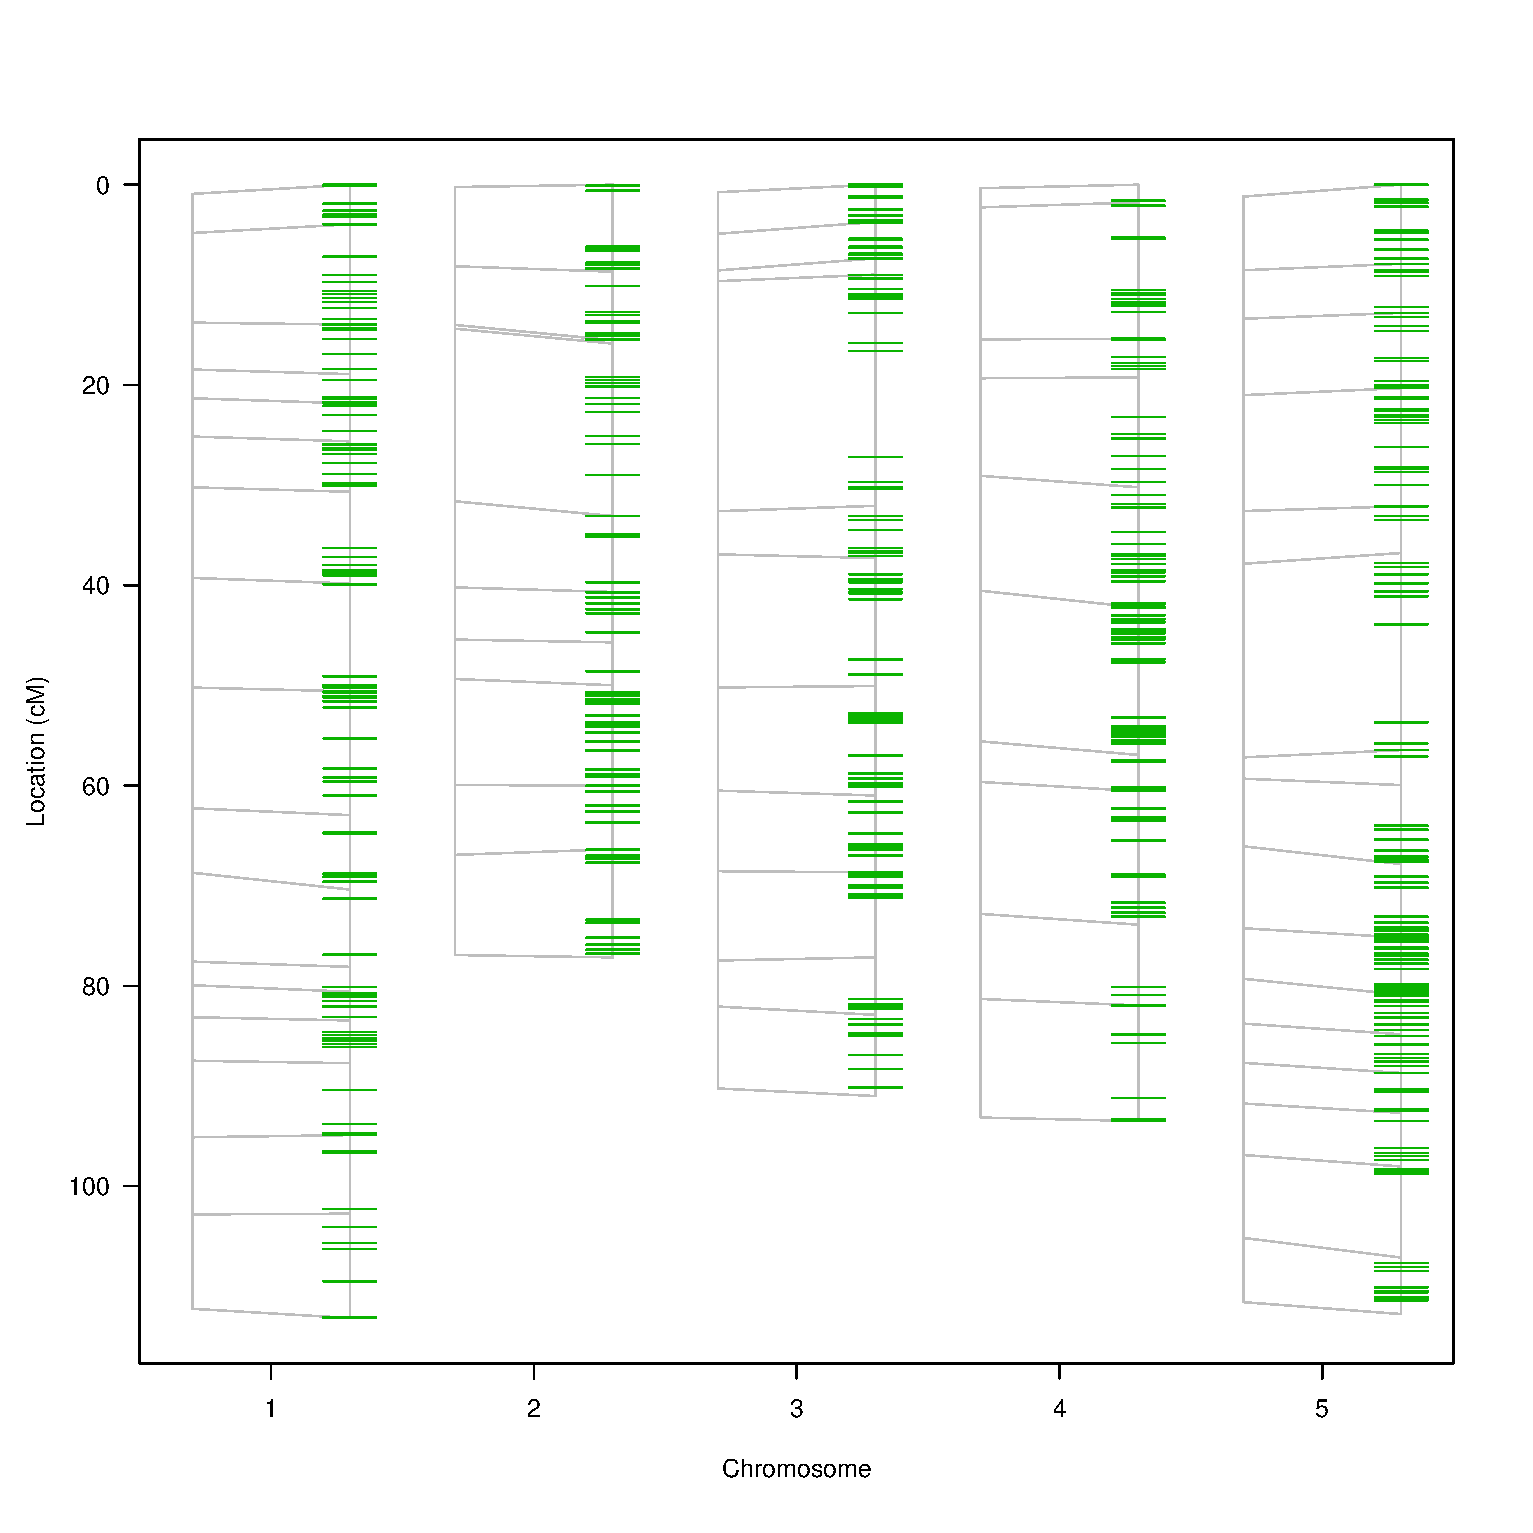
\includegraphics[keepaspectratio,scale=0.30]{eps/image_2_1.eps}
  \caption[Map comparison plot]{ Created with the R/qtl function \emph{plot.map} \cite{Broman:2003, 
  		  Arends:2010}. For each of the chromosomes the original map (left) and the saturated map (right) 
  		  are plotted. Lines are drawn to connect markers. Markers that exist in just one map and not the 
  		  other are indicated by short line segments on the right side. Before plotting, both maps were 
  		  re-estimated using the R/qtl function \emph{est.map}. The original map consists of 5 chromosomes 
  		  and 69 markers at an average distance of 7.1 cM. The saturated map consists of the original 69 
  		  markers plus 497 expression-based markers at an average marker distance of 0.89 cM.}
  		  \label{fig:mapcomparison}
\end{figure}

\begin{figure}[h!]
  \centering
  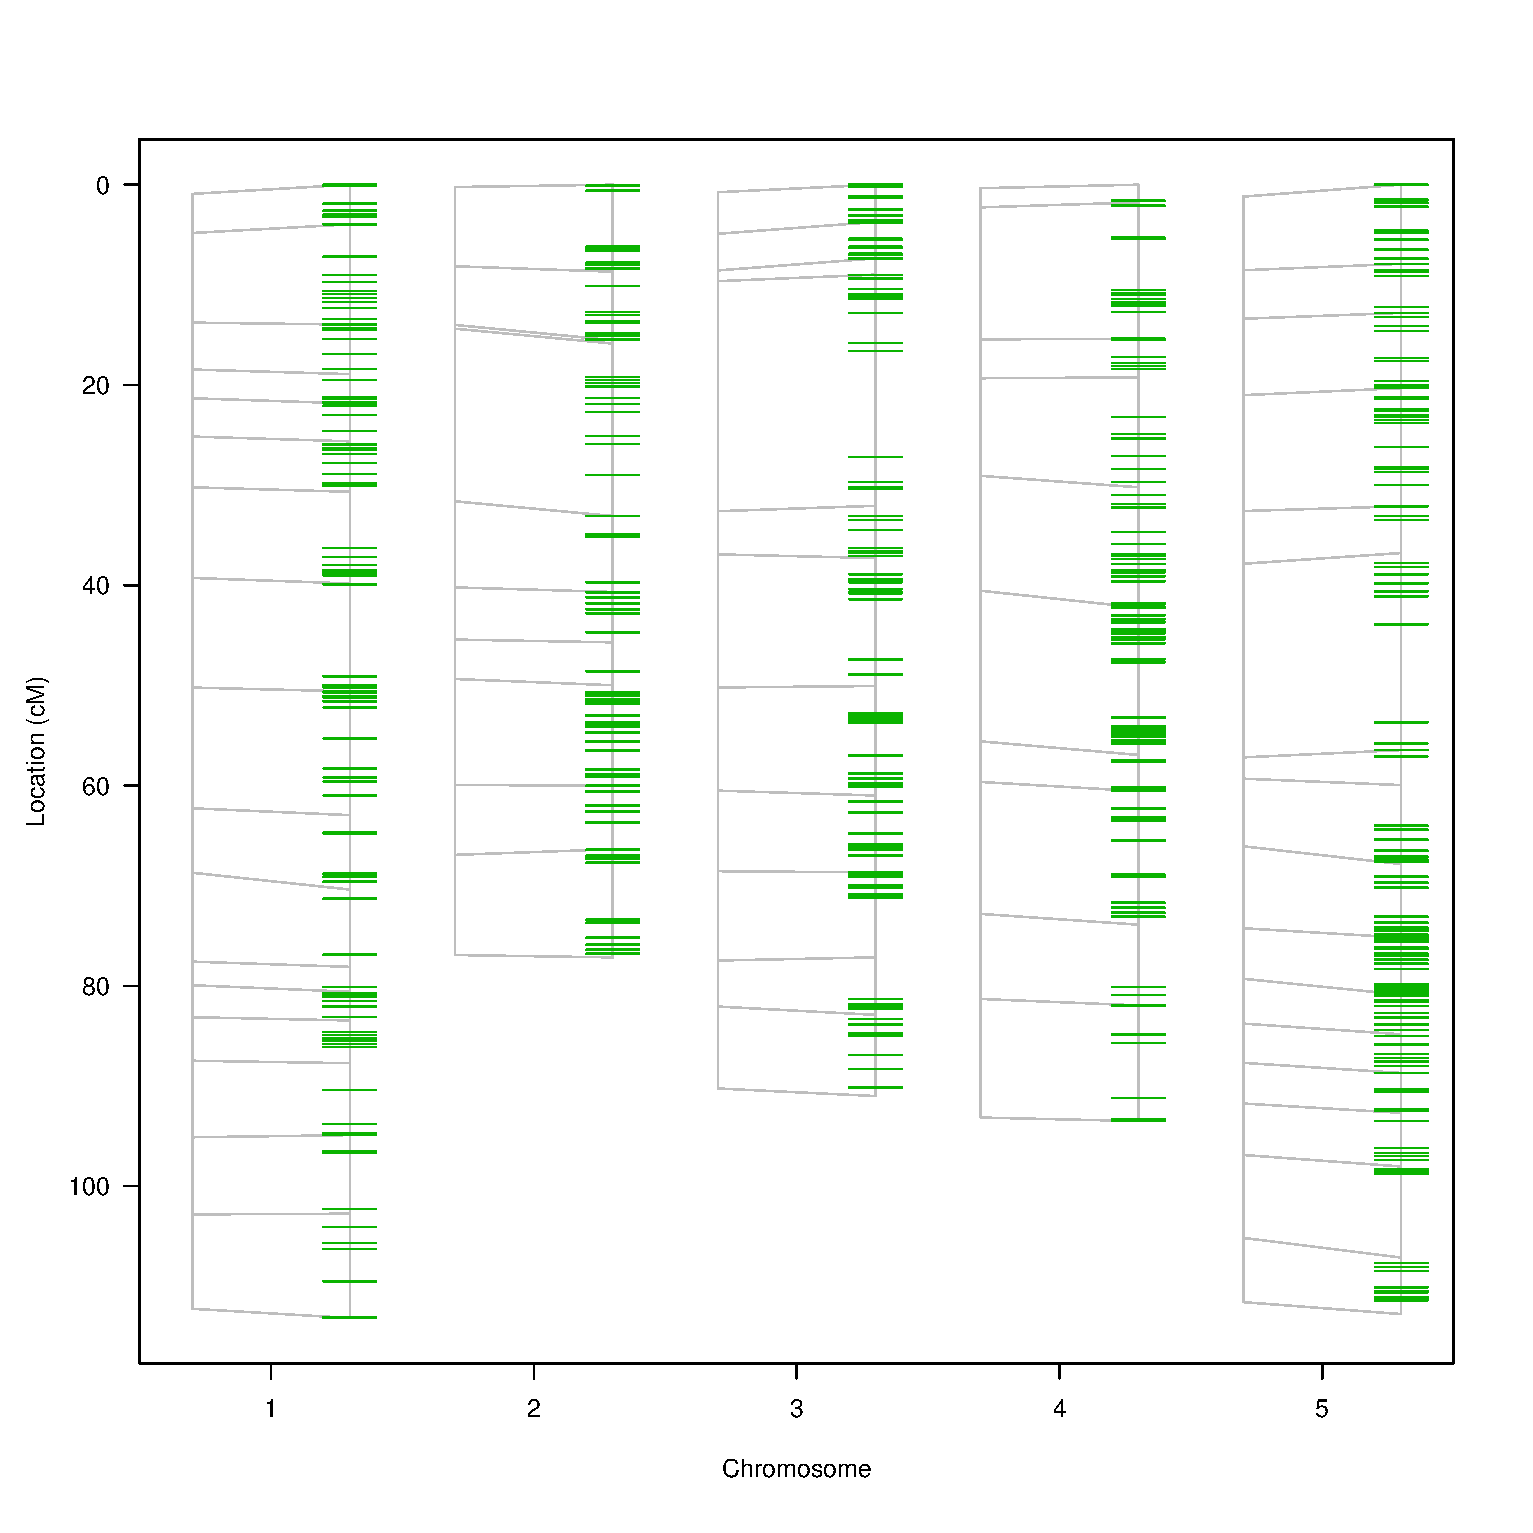
\includegraphics[keepaspectratio,scale=0.30]{eps/image_2_1.eps}
  \caption[Classical phenotype example.]{Results of single-marker QTL mapping of a classical phenotype on original (red 
          line) and saturated map (grey line)(left axis). Only chromosome 1 is shown. 
          {\bf Ticks on an X-axis} - positions of the original markers on the genetic map. 
          {\bf Black dots} - positions of the original markers on the physical map. 
          {\bf Colored dots and circles} - candidate markers detected by Pheno2Geno.
  		  {\bf Orange circles} - candidate markers removed because they showed significant environmental influence. 
  		  {\bf Blue circles} - candidate markers removed because they showed an epistatic interaction with other genetic markers. 
  		  {\bf Red dots} - markers used for saturation of the original map. The final saturated map consists of all the 
  		                   orange and black dots.
  		  Shown here are locations of the new markers on the old map, in this way maps align for better clarity.}
  		  \label{fig:qtlcomparison}
\end{figure}

\begin{figure}[h!]
  \centering
  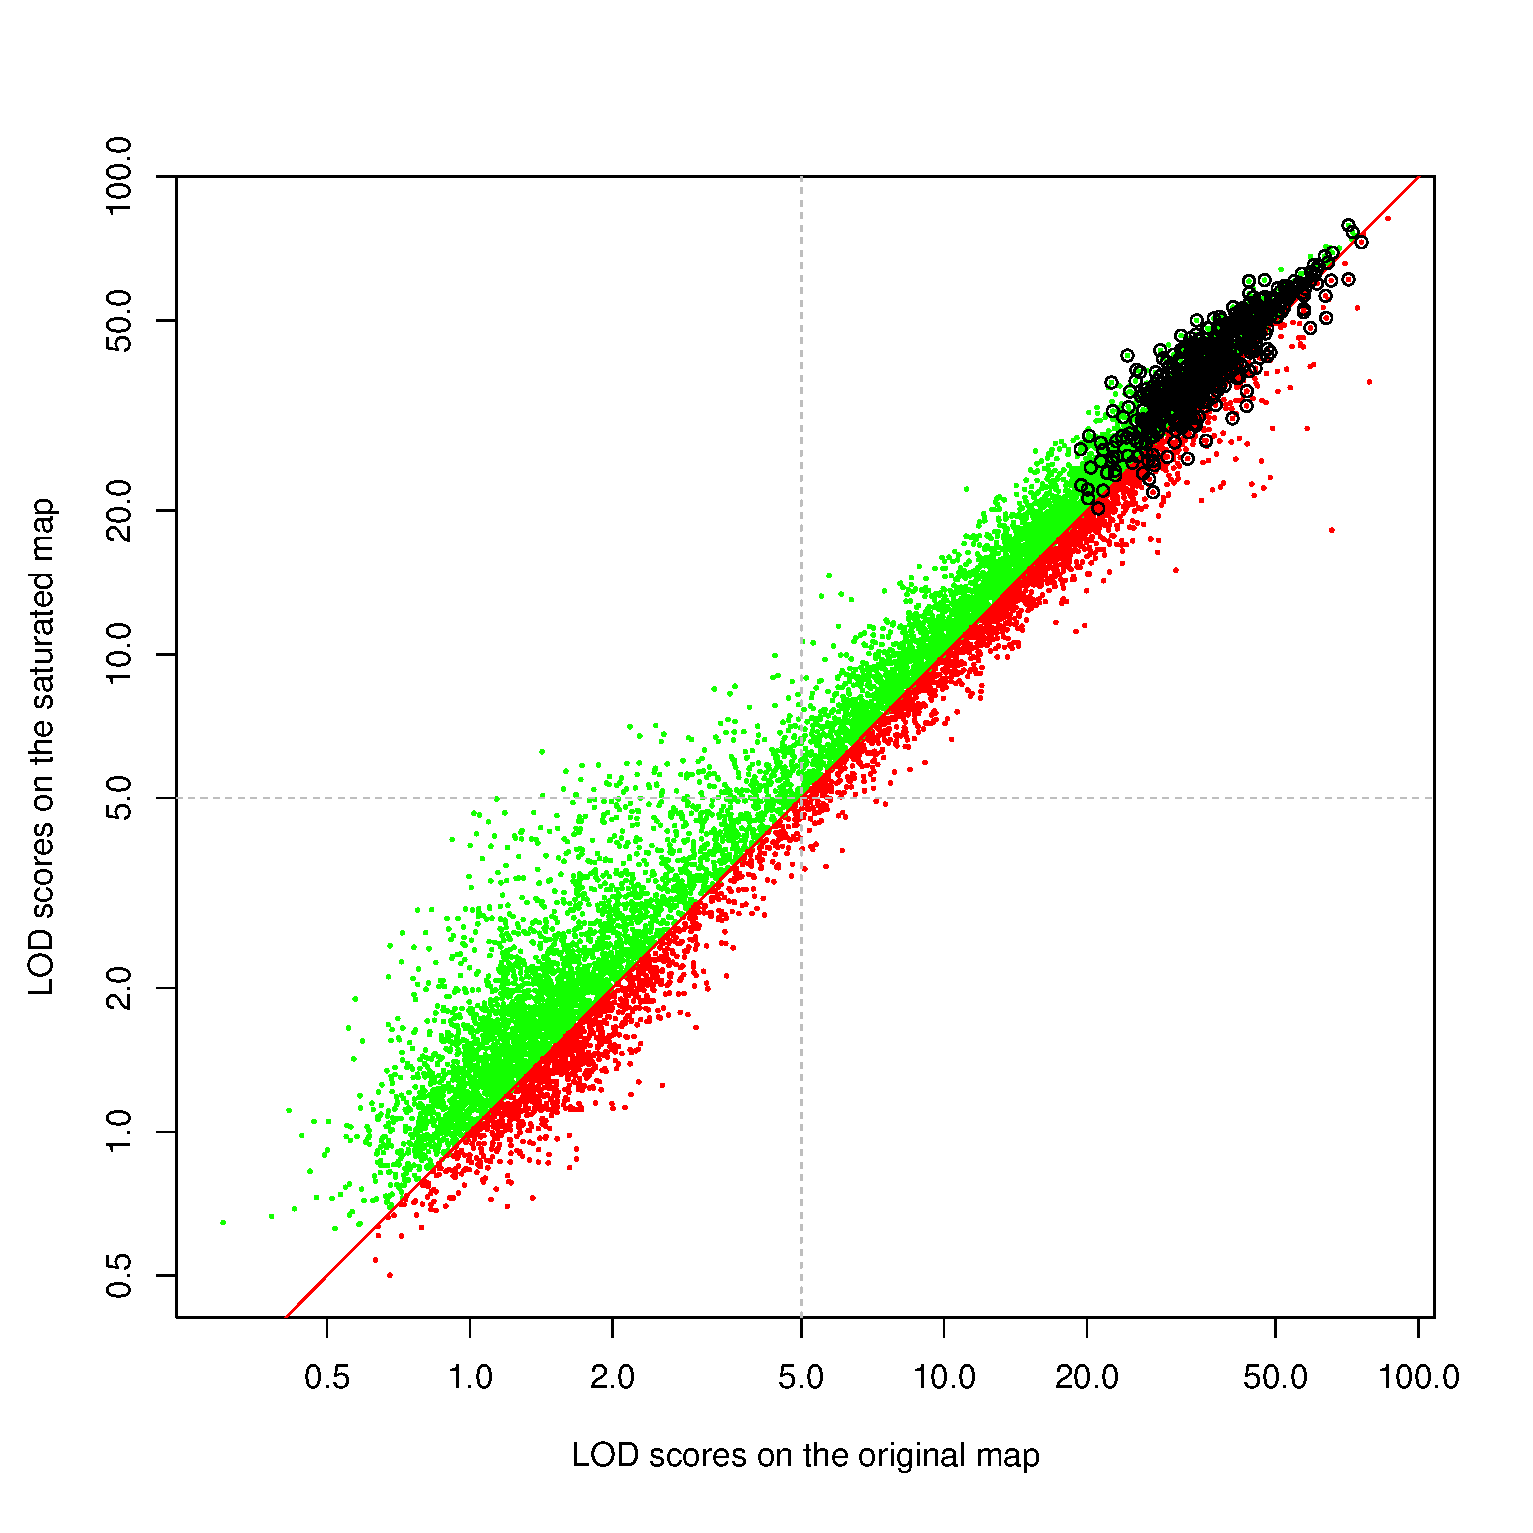
\includegraphics[keepaspectratio,scale=0.30]{eps/image_2_3.eps}
  \caption[LOD comparison.]{LOD scores on original and saturated map. QTL mapping was performed on all 10,801 SNP probes 
          showing differential expression between parents ($p < 0.01$ Student t-test) using original and saturated map. 
          5837 probes show a QTL with a $LOD > 5$ on  the original map. {\bf Orange dots} - 3943 probes (66\%) that show 
          an increased LOD score on the new saturated map. Moreover, 210 new QTLs were detected on the saturated map. 
          {\bf Black dots} -  probes showing a decrease in LOD score on the saturated map. {\bf Blue circles} - probes 
          used to saturate the map.}
          \label{fig:lodcomparison}
\end{figure}

\begin{figure}[h!]
  \centering
  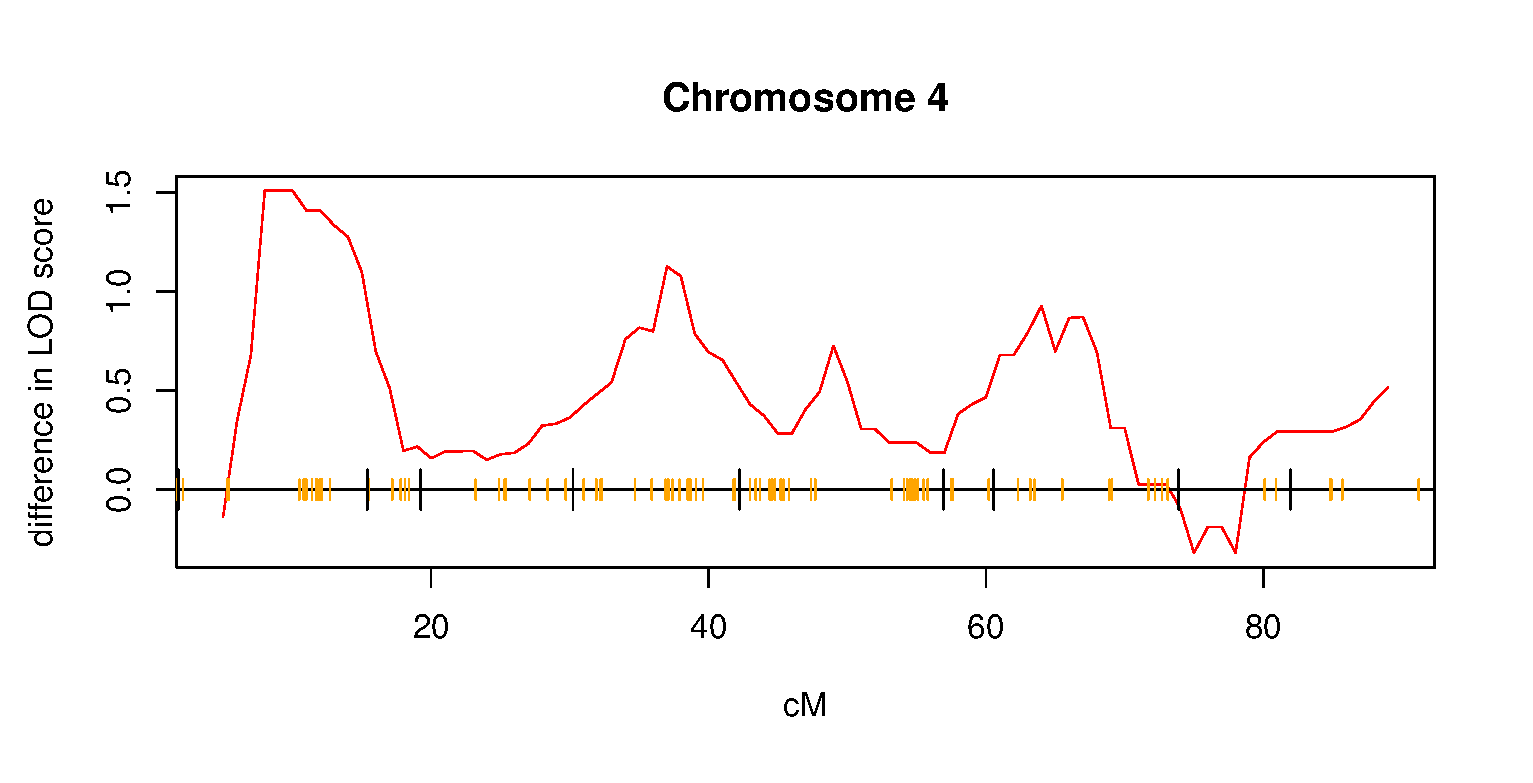
\includegraphics[keepaspectratio,scale=0.50]{eps/image_2_4.eps}
  \caption[LOD changes.]{Changing LOD scores. For each of the phenotypes the top QTL peak was selected. If the peaks 
  		  measured on original and saturated map shared location, the differences between LOD scores was calculated. 
  		  {\bf Solid red line} - median of differences between peaks from chromosome 4, calculated inside a sliding 
  		  window of 10 cM, moved across chromosome with a step of 1 cM. For each of the windows the value was plotted 
  		  in the middle of the compartment (hence no value for the first and the last 5 cM). Ticks on the x axis show 
  		  the position of the markers: {\bf black tall ticks} - original markers; {\bf orange short ticks} - markers 
  		  selected by Pheno2Geno. Only one region, when no new markers were added (75-80 cM) does not show increase in 
  		  power. }
  		  \label{fig:qtldetection}
\end{figure}

\section{Features}
Pheno2Geno provides the following functionality to saturate and create genetic maps:

{\bf 1) Preprocessing of the data}: Pheno2Geno offers a selection of 
data transformation functions (including: log, sqrt, reciprocal, probit and logit). 
Gene expression data measured using microarrays are for example generally log 
\cite{Quackenbush:2002} or square root\cite{Jansen:2001a, Gort:2010} transformed before 
further analysis.

{\bf 2) Analysis of parents of segregating population}: When parental data are available 
Pheno2Geno uses a \emph{t}-test to select molecular phenotypes showing significant 
differences between parental strains of segregating population. This reduces the computational load 
of the analysis.

{\bf 3) Analysis of segregating population}:
Phenotypes with a major QTL will show clear multimodal distributions in a segregating 
population. Pheno2Geno fits a mixture model to the phenotype distribution \cite{Jansen:1993, 
Jansen:2001a, Benaglia:2009}. Phenotypes are selected as candidate markers when 
significant multimodality is observed together with mixing proportions close to the expected segregation 
frequency, e.g. 1:1 for a bimodal distribution of two homozygous classes in 
a RIL; 1:2:1 for a trimodal distribution of two homozygous and one heterozygous class in 
an F2 cross.

{\bf 4) Assigning genotypes}:
The posterior probabilities of belonging to an underlying component distribution in the 
mixture is calculated for each component \cite{Jansen:2001b, Benaglia:2009}. Using these 
posterior probabilities, the continuous phenotype values are converted into discrete data 
(e.g. 0 or 1 for RILs; 0, 1 or 2 for F2).  If the posterior probability for a specific 
marker-individual combination is lower than a user-specified threshold, a missing value 
(*) or partly informative value (e.g. not 0, but homozygous 2 or heterozygous 1) is 
assigned to avoid introducing genotyping errors. If parental data is available these can 
be given a parental origin label (A or B for RILs, A, H or B for F2). 
When parental data are not available, mixture-model based scores cannot be converted into 
parental origin labels. Pheno2Geno is able to solve that in case of RILs by forming twice 
as many linkage groups compared to the expected number of chromosomes and then merges 
anti-correlated pairs of linkage groups into a single chromosome.

{\bf 5) \emph{De-novo} construction of genetic maps}: 
When no initial map is available, Pheno2Geno can be used to create an initial 'skeleton' 
map. This skeleton map is produced using very strict settings in the mixture model 
analysis to obtain a limited number of highly trustworthy markers. These candidate markers 
are assigned to linkage groups using the R/qtl function \emph{formLinkageGroups}. 
Additional information provided by the user is used in this step, e.g. known physical 
and genetic positions will be used by Pheno2Geno to assign physical chromosome IDs to 
linkage groups and to determine the correct orientation of chromosomes. The package then 
orders all the markers inside a linkage group by using the R/qtl \emph{orderMarkers} 
function. Finally the skeleton map is saturated to improve resolution as described in 
the next section.

{\bf 6) Environment and epistasis}: 
West et al. \cite{West:2007} emphasized that creation of genetic markers from gene expression data 
is seriously hampered by the presence of environmental variation and multiple possibly interacting 
QTLs (epistasis) suing R/qtl. Pheno2Geno tests if candidate markers are affected by multiple QTLs or pairwise 
interactions. When data were collected in multiple environments potential environmental interactions 
are tested. The user decides whether affected candidate markers are flagged or removed from further analysis.

{\bf 7) Saturation of a known map}:
Pheno2Geno performs interval mapping (using the R/qtl \emph{scanone} function) of 
candidate markers on the original map. The candidate markers are placed on the position 
of the QTL peak. The map is re-estimated (using the R/qtl \emph{est.map} function). 
Followed by  removal of duplicate candidate markers and markers located at the position 
of a known marker.

{\bf 8) Detection of errors}:
After saturation or \emph{de-novo} construction of a genetic map, Pheno2Geno can detect 
and correct genotyping errors (e.g. double recombinations, missing data, semi informative 
markers) using the R/qtl function \emph{fill.geno}. Furthermore, when saturating a known 
map with available genotype data, Pheno2Geno can detect sample mix-ups in the 
original data using R/lineup (which is part of the R/qtl toolset). Users can also use 
external tools such as MixupMapper \cite{Westra:2011} beforehand to detect and correct the 
original genotype data.

\section{Results}
In order to test our package, we performed an analysis of a population with a sparse map.
The original AFLP map was created using a population of 420 RILs derived from a cross between 
\emph{Arabidopsis thaliana} Bayreuth (Bay-0) x Shahdara (Sha) \cite{Loudet:2002}. 
Our dataset consists of 164 RILs from the core population, which were assigned to 4 conditions 
using the designGG package\cite{Li:2009}. Parents were measured in duplicate per condition. 
Gene expression was measured on 370,000 transcripts. During Quality Control 16 arrays 
(all RILs) were discarded, leaving 148 RILs and 16 parental arrays for further analysis.

The original map contained 69 AFLP markers at an average map distance of 7.1 cM\cite{Loudet:2002}. 
Resolution of a genetic map is limited by the size of the population from which the map is derived. 
A distance of 1 cM is equal to 1 recombination in a 100 individuals. Our sample size of 148 
individuals implies that we can obtain at best a resolution of 0.68 cM between markers.

10,801 phenotypes are detected as being differentially expressed between parents 
($P < 0.01$). Mixture modeling identified 1,230 potential markers showing approximately 1:1 
segregation ratio. Pheno2Geno removed 267 markers which show QTL by environment interaction
($LOD >= 7.5$), and 286 candidate markers which show none ($LOD < 15$) (279 markers) or 
multiple QTL (7 markers). Scanning for epistasis showed 77 candidate markers which appear to 
show pairwise epistatic interactions ($LOD >= 7.5$). 

Using the remaining 600 candidate markers the original map was saturated, and 103 co-localizing 
markers were removed. This resulted in 497 new gene expression based markers (720\% increase). 
ap distances were re-estimated (est.map) using the Kosambi's map function. Map expansion was 
observed on chromosomes 4 and 5 increasing total map length from 480.7 to 501.5 
cM (Fig. \ref{fig:mapcomparison}). Nonetheless, the saturation resulted in decreasing the average map distance 
from 7.1 cM to 0.89 cM. This is close to the theoretical resolution limit (0.68 cM) given 
the size of population. Saturation of the \emph{A. thaliana} Bay-0 x Sha map led to a more 
than sevenfold improvement in marker density at no additional lab cost. 

A \emph{de-novo} reconstruction using gene expression data only (ignoring the original 
markers and map) would have led to a skeleton map containing 227 markers with average 
distance of 2.2 cM. 

Additionally, we performed a QTL mapping of our previously published classical 
phenotype dataset\cite{Joosen:2011} onto the saturated map. This showed an increase in QTL 
likelihood for 56\% of previously detected QTLs. Additionally, 29 new QTLs were detected 
on the saturated map. These QTLs showed LOD scores close to the threshold when mapped 
onto the original map ($ 3.4 <= LOD <= 5$, Fig. \ref{fig:qtlcomparison}).

Finally,  a QTL mapping of all the gene expression probes showing differential expression 
between parents (10,801 probes) was performed. 5,837 probes had a significant ($LOD > 5$) 
QTL on the original map. Out of these, 3,943 probes (66\%) showed an increase in QTL 
likelihood on the saturated map (Fig. \ref{fig:qtldetection}) and additional 210 new significant QTLs are 
detected on the saturated map.
  
\section{Conclusions and Discussion}
Pheno2Geno is a generic software package for generating genetic markers and maps from 
high-throughput molecular phenotypes for any inbred diploid population (e.g: backcross, 
F2 intercross and recombinant inbred lines). Pheno2Geno has four important features which 
we will discuss one by one:

{\bf 1) Big data computation.}
Pheno2geno can process large volumes of different kinds of molecular phenotypes \cite{Trelles:2011}. 
Memory requirements of the algorithm are decreased by reading in and processing 
files in chunks rather than at once. Complete analysis of the showcase data (370,000 transcripts) 
is performed under an hour on an average desktop PC (Intel Core i5, 4 GB of RAM). For even larger 
datasets, the Pheno2Geno package is embedded in xQTL workbench \cite{Arends:2012, Snoek:2012} 
allowing for easy parallelization, use of cluster and cloud computing.

{\bf 2) Integration with R/qtl.}
The package is employing well optimized methods and functions of R/qtl for all the mapping steps,
filling and (re)estimation of maps. Moreover, genetic maps created by Pheno2Geno can be directly 
used in R/qtl, providing a smooth transition from genetic map creation to QTL mapping.

{\bf 3) Strict selection of candidate markers.}
The analysis of Pheno2Geno contains multiple selection steps filtering out candidate markers of 
low quality. E.g. candidate markers affected by multiple QTLs and/or environment are flagged and 
can easily be excluded from the analysis.

{\bf 4) Gene expression phenotypes.}
We have illustrated Pheno2Geno on array-based gene expression data. If a gene expression 
phenotype shows a significant QTL (eQTL) and if this eQTL co-localizes with the probe (a 
local eQTL), then the derived marker will be mapped at the location of the probe. The eQTL 
may actually be caused by polymorphisms in the region targeted by the probe \cite{Alberts:2005, 
Alberts:2007}. If the QTL does not lo-localize with the probe (a distant eQTL), the derived 
marker will not be located at the region targeted by the original probe but correctly at the 
position of the distant eQTL.



\chapter{High throughput (Multiple) QTL mapping}
\thispagestyle{empty}
\label{chap:mqm}

\emph{QTL mapping is the main analysis method used in the analysis of quantitative traits. This 
approach has been the analysis method to study quantitative traits since its discovery in 1980. 
Many variations to the basic single marker approach can be made, but none so fundamental as 
multiple QTL mapping using generalized lineair models. Computational and sample size problems 
were limiting the application of the approach. Novel experimental design and decreased costs 
have made sample size less of an issue, and by 'refreshing' the original algorithm more 
wide-spread application of this important algorithm is possible.}
\null
\vfill

\begin{myexampleblock}{Originally published as:}
  \authors{Danny Arends*, Pjotr Prins*, Ritsert C. Jansen and Karl W. Broman}\\
  \emph{R/qtl: High throughput Multiple QTL mapping}\\
  \bold{Bioinformatics} (2010) \\

  \authors{Danny Arends*, Ronny V. L. Joosen*, Leo Willems, Wilco Ligterink, Henk Hilhorst, Ritsert C. Jansen}\\
  Visualizing the genetic landscape of Arabidopsis seed performance\\
  \bold{Plant Physiology} (2011)\\

  \authors{Danny Arends*, Ronny V. L. Joosen*, Yang Li*, Leo Willems, Joost J.B. Keurentjes, Wilco Ligterink, 
  Ritsert C. Jansen, Henk Hilhorst}\\
  Identifying genotype-by-environment interactions in the metabolism of germinating Arabidopsis seeds using 
  Generalized Genetical Genomics\\
  \bold{Plant Physiology} (2013)
\end{myexampleblock}

\newpage

Here we show he contributions made to R/qtl and show the application of our newly developed toolset 
to map genetic variation underlying classical phenotypes in \emph{A. thalaina} seed development. We 
show that by using a reduced number of individuals using the designGG strategy we can map main- and 
interactioneffects with more statistical power compared to other designs. After this we use a limited 
number of individuals and continue our analysis by zooming into the metabolic level, we show that 
there are shared genetic loci between phenotypes at different bio-molecular levels. Additional using 
the new optimized MQM routine allows us to detect more loci and/or give more confidence in the loci 
detected.

\section{Single marker QTL mapping (R/qtl)}
R/qtl is an extensible, interactive environment for the mapping of quantitative trait loci (QTL) 
in experimental crosses. It is implemented as an add-on package for the freely available and 
widely used statistical language/software R \cite{R:2009}. Since its introduction, R/qtl 
\cite{Broman:2003} has become a reference implementation with an extensive guide on QTL mapping 
\cite{RQTLGuide:2009}. R/qtl development is continuous, with input from multiple collaborators 
and users.  We have introduced a full testing environment with regression testing, updated the 
license to the GPL version 3, and hosted the source code repository on Github, which gives R/qtl 
software development high visibility and transparency. 

The development of R/qtl reflects trends in quantitative genetics, in particular the use of 
larger datasets, larger calculations and requirements for controlling the false discovery rate. 
These developments are partly driven by high-throughput genetical genomics the name coined 
for the study of gene expression QTL (eQTL)\cite{Jansen:2001a}, metabolite QTL (mQTL), protein 
QTL (pQTL).

\section{Multiple QTL mapping}
Multiple QTL Mapping (MQM) belongs to a family of QTL mapping methods, that include Haley-Knott 
regression \cite{Haley:1992} and composite interval mapping CIM \cite{Zeng:1994}. MQM combines 
the strengths of generalized linear model regression with those of interval mapping 
\cite{Jansen:1993, Jansen:1994b}. 

Recent developments in QTL mapping include Bayesian modeling of multiple QTL e.g. R/qtlbim 
package \cite{Yandell:2007, Banerjee:2008}. Bayesian modeling, however, is computationally 
expensive, and arguably has little additional power when applied to high density maps, and 
(nearly) complete genotype data \cite{Handbook:Jansen:2007}. Still, we intend to combine the 
strengths of the different methods in future versions of R/qtl.

These days, with most experimental setups and high density maps, improving precision may be 
achieved by increasing the population size first. For more information on QTL mapping and 
Bayesian analysis we refer to the `Handbook of Statistical Genetics` \cite{Handbook:2007}. MQM 
makes used of generalized linear models, thereby potentially providing unified analysis of 
non-normal traits.

MQM provides a practical, relevant and sensitive approach for mapping QTL in experimental 
populations. The theoretical framework of MQM was introduced and explored by R.C. Jansen 
\cite{Jansen:1994a} and explained in the 'Handbook of Statistical Genetics' 
\cite{Handbook:Jansen:2007}. MQM has one known commercial implementation \cite{Mapqtl:2002}, 
which has been used effectively in practical research, resulting in hundreds of papers, e.g., 
in mouse, plant, and fish, respectively \cite{DeMooij:2009, Jeuken:2009, Kitano:2009}. Now, 
with MQM for R/qtl, we present the first free and open source implementation of MQM, that is 
multi-platform, scalable and suitable for automated procedures and large datasets.

\subsection{Features}
MQM for R/qtl is an automated three-stage procedure in which, in the first stage, missing 
genotype data is 'augmented'.  In other words, rather than guessing one likely genotype, 
multiple genotypes are modelled with their estimated probabilities. In the second stage, 
important marker cofactors are selected by multiple regression and backward elimination. 
The third stage, a QTL is moved along the chromosomes using these pre-selected markers as 
cofactors (Fig. \ref{fig:comparison}). QTL are interval-mapped using the most informative 
model selected by either maximum likelihood or restricted maximum likelihood. A refined 
and automated procedure for cases with large numbers of marker cofactors is included. 

\begin{figure}[h!]
  \centering
  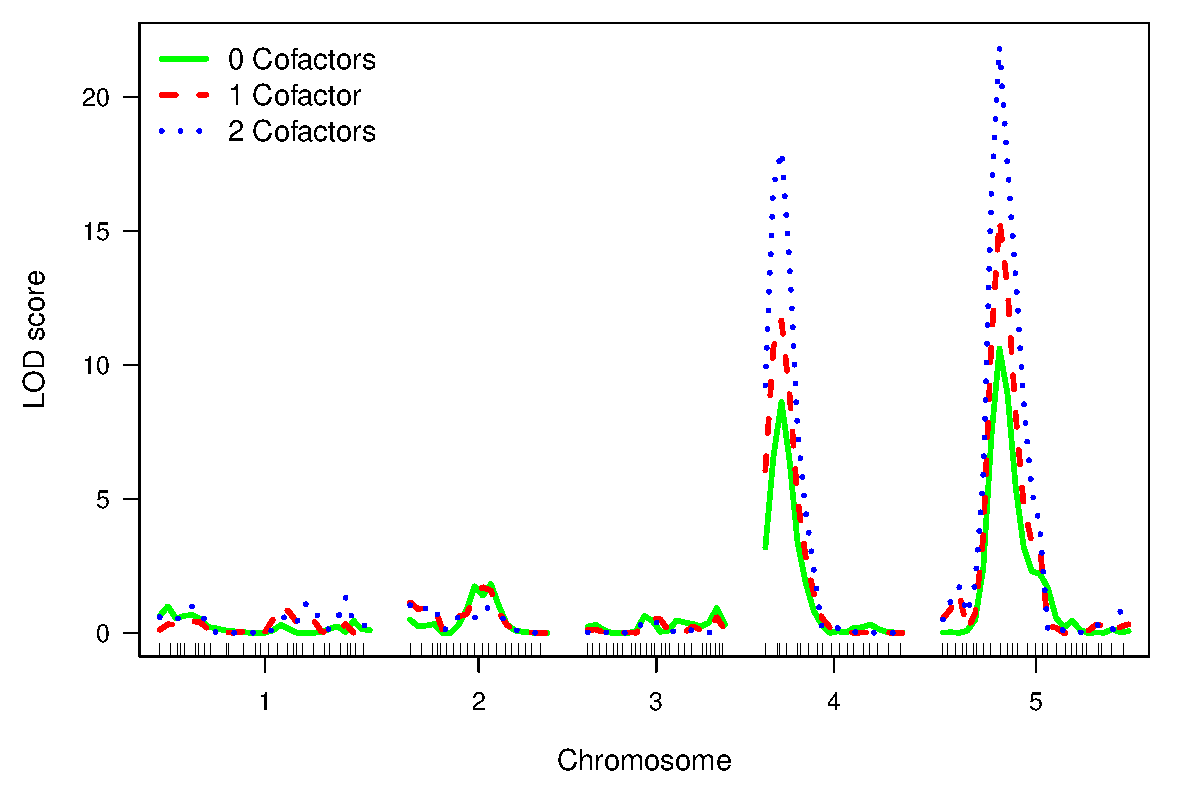
\includegraphics[keepaspectratio,scale=0.30]{eps/image_3_3.eps}
  \caption[Comparison of QTL mapping methodologies.]{ Three way comparison of MQM performance in {\it Arabidopsis 
          thaliana} \citep{Fu:2007}. LOD score increases when cofactors are added manually to the model. Here, 
          adding more than two cofactors does not improve the model any further (as discussed in the online 
          MQM tutorial).}
  \label{fig:comparison}
\end{figure}

The method lets users test different QTL models by elimination of non-significant cofactors. 
MQM for R/qtl brings the following advantages to QTL mapping:
\begin{enumerate}\itemsep1pt
\item Higher power, as long as the QTL explain a reasonable amount of variation.
\item Protection against over-fitting, because MQM fixes the residual variance from the full 
model, which allows the use of more cofactors than may be used in, for example, composite 
interval mapping \cite{Zeng:1994}.
\item Prevention of ghost QTL detection (between two QTL in coupling phase).
\item Detection of negating QTL (QTL in repulsion phase). 
\item MQM gives (compared to CIM) a reduction in type I and type II error \cite{Handbook:Jansen:2007}.
\item A pragmatic permutation strategy for controlling the false discovery rate (FDR) and 
prevention of locating false QTL hot spots, as discussed in Breitling et al \cite{Breitling:2008a}. 
Marker data is permuted, while keeping the correlation structure in the trait data.
\item High-performance computing by scaling on multi-CPU computers, as well as clustered 
computers, by calculating phenotypes in parallel, through the Message Passing Interface (MPI) of 
the SNOW package for R\cite{Tierney:2009}.
\item Visualizations for exploring interactions in a genomic circle plot (Fig. \ref{fig:circleplot}) and \emph{cis}- 
and \emph{trans}-regulation (Fig. \ref{fig:cistrans}).
\end{enumerate}

\begin{figure}[h!]
  \centering
  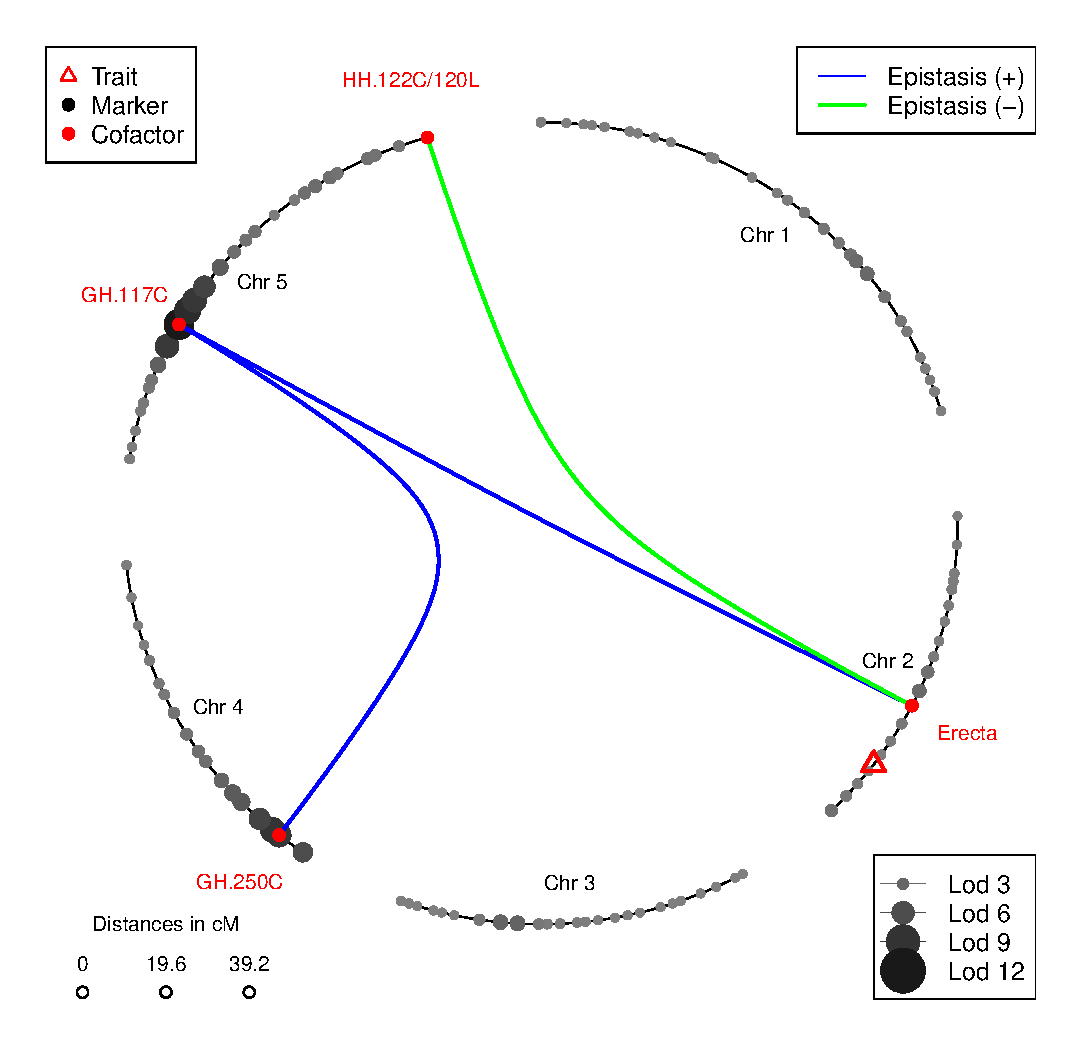
\includegraphics[keepaspectratio,scale=0.30]{eps/image_3_1.eps}
  \caption[Circle plot.]{Circular genome interaction plot \textcolor{black}{of the {\it Arabidopsis 
        thaliana} glucosinolate pathway} \citep{Fu:2007}.  LOD scores shown at marker positions 
        are scaled (grey circles), with selected cofactors (red circles) and epistasis between 
        multiple cofactors (green and blue splines)..}
  \label{fig:circleplot}
\end{figure}

\begin{figure}[h!]
  \centering
  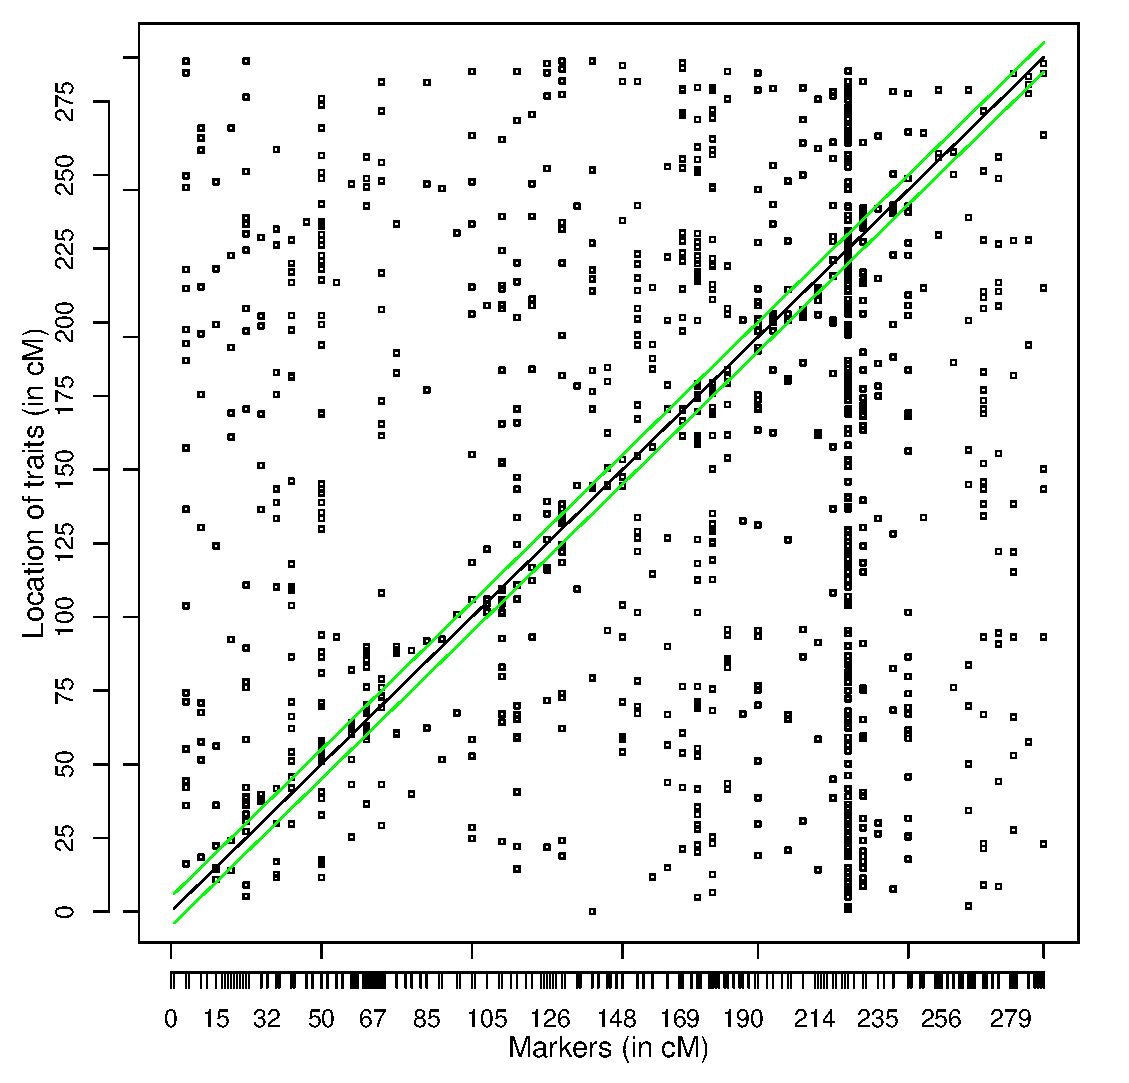
\includegraphics[keepaspectratio,scale=0.30]{eps/image_3_2.eps}
  \caption[CisTrans plot.]{Cis-trans plot of significant QTL (squares) showing cis acting QTL (diagonal) 
          and a trans-band (vertical, chromosome 5) in {\it Caenorhabditis elegans} \citep{Li:2006}.}
  \label{fig:cistrans}
\end{figure}

A 40-page tutorial for MQM explores, both the automated procedure, and the manual procedure 
of adding and removing cofactors, in an \emph{Arabidopsis thaliana} recombinant inbred line 
(RIL) metabolite (mQTL) dataset with 24 metabolites as phenotypes \cite{Fu:2007}. In addition, 
the tutorial visually explains the effects of data augmentation, cofactor selection, model 
selection, and tweaking of input parameters, such as cofactor significance. Genetic interactions 
(epistasis) are explored through effect plots, and an example is given of parallel computation. 
The tutorial is part of the software distribution of R/qtl and is available online.

\subsection{Conclusions and Discussion}
MQM for R/qtl is a significant addition to the QTL mapper's toolbox. R/qtl provides the user 
with the most frequently used statistical analysis methods: single-marker analysis, interval 
mapping, Haley-Knott regression \cite{Haley:1992}, CIM \cite{Zeng:1994} and MQM \cite{Jansen:1994a}. 
MQM has improved handling of missing data and allows more powerful and precise detection of QTL, 
compared to many other methods. Not only is this new implementation of MQM available in the
statistical R environment, which allows scripting for pipe-lined setups, it is also highly 
scalable through parallelisation and paves the way for high-throughput QTL analysis. With MQM, 
R/qtl is a free and high-performance comprehensive QTL mapping toolbox for the analysis of 
experimental populations. R/qtl now includes permutation strategies for determining thresholds 
of significance relevant for QTL and QTL hot spots; the first step towards causal inference and
network analysis.



\section{Mapping classical phenotypes}
Perfect timing of germination is required to encounter optimal conditions for plant survival and it 
is the result of a complex interaction between molecular processes, seed characteristics and 
environmental cues. To detangle these processes we made use of natural genetic variation present in 
an Arabidopsis thaliana Bayreuth x Shahdara RIL population. For a detailed analysis of the germination 
response we characterized rate, uniformity and maximum germination and discussed the added value of 
such precise measurements. The effects of after-ripening, stratification and controlled deterioration 
as well as the effect of salt (NaCl), mannitol, heat, cold and ABA with and without cold stratification 
were analyzed for these germination characteristics. Seed morphology (size, length) of both dry and 
imbibed seeds were quantified by using image analysis. For the overwhelming amount of data produced 
in this study we developed new approaches to perform and visualize high throughput QTL analysis. 
We show correlation of trait data, (shared) QTL positions and epistatic interactions. The detection 
of similar loci for different stresses indicate that often the molecular processes regulating 
environmental responses converge into similar pathways. 7 major QTL hotspots were confirmed using a 
HIF approach. QTLs co-locating with previously reported QTLs and well characterized mutants are 
discussed. A new connection between dormancy, ABA and a cripple mucilage formation due to a natural 
occurring mutation in the MUM2 gene is proposed and this is an interesting lead for further research 
on the regulatory role of ABA in mucilage production and its multiple effects on germination parameters.

\subsection{Background}
Colonizing plants are subject to a wide variety of environmental conditions. For successful adaptation 
to new habitats the timing of developmental transitions is especially important. Seed germination is 
one of these important transitions as it determines the seasonal environment experienced in further 
plant life \cite{Huang:2010}. Natural populations that develop under distinct environmental conditions 
may reveal genetic adaptation, which can be used to disentangle the signaling routes that are involved. 
Seed germination is described by three phases of water uptake. In phase I the seeds imbibes and 
reinitiates metabolic processes followed by a lag phase (phase II). Further water uptake results in 
protrusion of the radicle through the testa and endosperm (phase III). The moment of radicle 
protrusion through the endosperm is considered to be the moment of germination sensu stricto 
\cite{Finch-Savage:2006}. To characterize the genetic variation of germination related traits we 
focused on the effect of the environment that a seed perceives during germination rather than the 
effect of the environment during maternal plant growth, which has been the subject of other 
studies \cite{Dechaine:2009, Elwell:2011}. 

\begin{figure}[!ht]
  \centering
  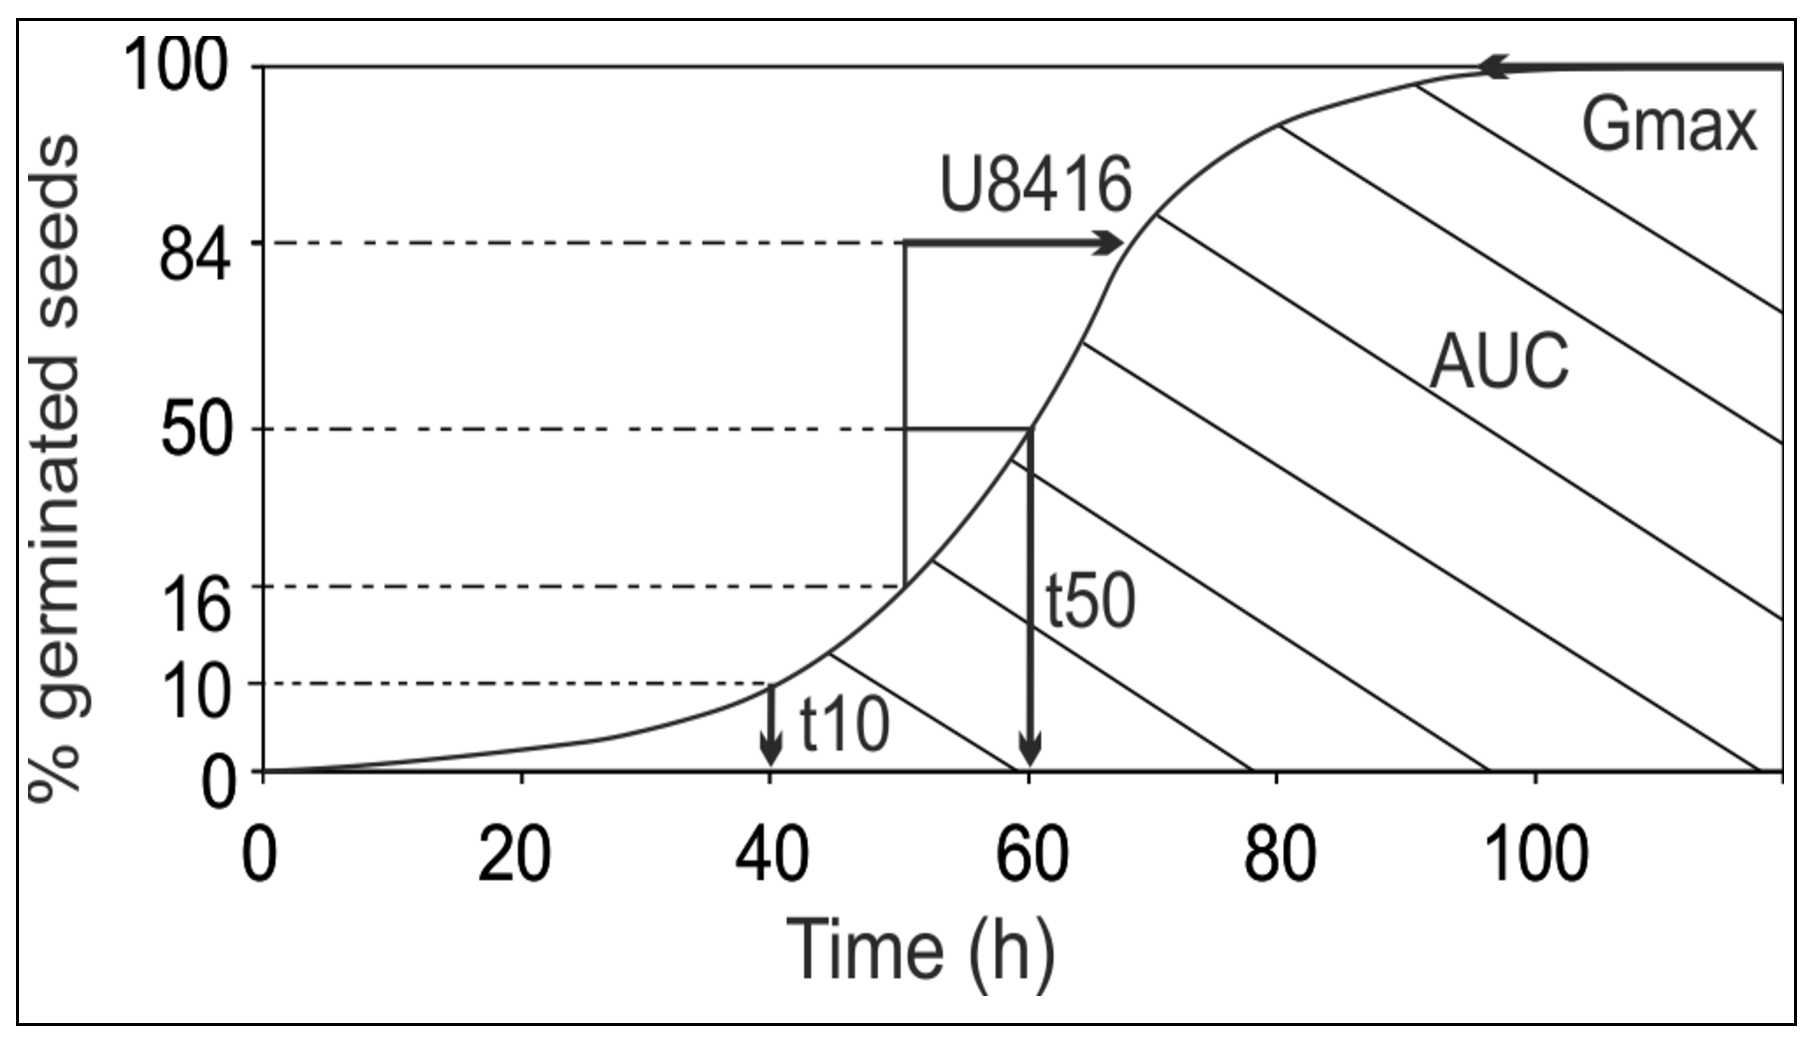
\includegraphics[keepaspectratio,scale=0.30]{eps/image_3_1_1.eps}
  \caption[Germination curve]{A hypothetical germination curve, $t_{10}$: Time when 10\% of seeds have 
          germinated, $t_{50}$: Time when 50\% of seeds have germinated. $U_{8416}$,  Uniformity of 
          germination, time difference between 16\% germination and 84\% germination. $G_{max}$: \% of 
          germinated seeds, AUC: Area under the curve. }
  \label{fig:GerminationCurve}
\end{figure}

Seed content (e.g. oil) is often used as commodity and modifications to the content can therefore be 
regarded as seed quality parameters as well. To prevent confusion we will use the term seed performance 
to indicate that the focus of our study was restricted to seed germination characteristics.

The production of high quality crop seed not only entails knowledge about maternal plant growth, 
harvesting and storage of seeds, but also of germination conditions \cite{Rivero-Lepinckas:2006}. 
To obtain better germination and field performance, many seed companies rely on enhancement methods, 
such as seed priming and coating and/or pelleting, but these methods are reaching their limits. 
Dissecting the molecular mechanisms underlying seed germination and its tolerance to the environment 
may unlock the full genetic potential and enable targeted breeding for seed performance. In this study 
we used a recombinant inbred line (RIL) population derived from two \emph{Arabidopsis thaliana} ecotypes: 
Bayreuth (Bay-0) which originates from a fallow land habitat in Germany and Shahdara (Sha) which 
grows at high altitude in the Pamiro-Alay mountains in Tadjikistan \cite{Loudet:2002}. The Bay-0 x 
Sha RIL population has been used in many previous studies to map QTL positions for root morphology 
\cite{Loudet:2005, Reymond:2006}, anion content \cite{Loudet:2003a}, nitrogen use efficiency 
\cite{Loudet:2003b}, cell wall digestibility \cite{Barriere:2012}, carbohydrate content 
\cite{Calenge:2006}, sulfate content \cite{Loudet:2007}, leaf senescence \cite{Diaz:2006}, 
morning-specific growth \cite{Loudet:2008} and cold-dark germination \cite{Meng:2008}. We have used 
the natural variation present in this RIL population to map the response of germination characteristics 
to environmental conditions to which a seed is exposed.

\begin{table}[h]
  \centering
  {\footnotesize
  \begin{tabular}{  l  l  l  l  l  l }
    \hline
    {\bf Trait} & {\bf $G_{max}$} & {\bf AUC} & {\bf $t_{50}$}& {\bf $t_{10}$}& {\bf $U_{8416}$}\\
    \hline
    AR.NS           & 0.82 & 0.97 & 0.86 & 0.79 & 0.82 \\
    AR.NS.Cold      & 0.51 & 0.77 & 0.73 & 0.66 & 0.48 \\
    AR.NS.Mannitol  & 0.61 & 0.79 & 0.70 & 0.55 & 0.62 \\
    AR.NS.NACL      & 0.90 & 0.94 & 0.80 & 0.76 & 0.43 \\
    AR.WS           & 0.63 & 0.19 & 0.78 & 0.72 & 0.72 \\
    AR.WS.NACL      & 0.91 & 0.93 & 0.86 & 0.78 & 0.70 \\
    Fresh.NS        & 0.92 & 0.94 & 0.81 & 0.70 & 0.76 \\
    Fresh.WS        & 0.40 & 0.81 & 0.87 & 0.84 & 0.76 \\
    \hline
  \end{tabular}
  }
  \caption[Heritability Overview]{Overview of the broad sense heritability scores. Included are those traits 
          for which different blocks were tested (Trait code descriptions can be found in Table \ref{table:codes}, 
          for germination parameters see Figure \ref{fig:GerminationCurve}). Broad-sense heritability were 
          calculated with the QTL data analysis tools in Genstat 14, using the preliminary single environment 
          analysis and adding the block as an additional fixed term.}
\end{table}

Freshly harvested viable \emph{Arabidopsis} seeds often don't germinate even when placed under conditions 
favorable for germination. This event, called primary dormancy, is shown to be subject to natural 
variation \cite{Bentsink:2010}. In many \emph{Arabidopsis} ecotypes, this primary dormancy is released after 
a period of dry storage at room temperature. Another dormancy breaking treatment is cold stratification 
were seeds are imbibed in water and stored at 4\degree C in the dark for four days before putting them into 
optimal conditions for germination \cite{Finch-Savage:2006}. Unfavorable conditions during seed 
germination may result in a changed rate or even failure of germination. In \emph{Arabidopsis}, it has been 
shown that the responsiveness to temperature is closely related to the level of after-ripening 
\cite{Tamura:2006}. High salt concentrations induce osmotic stress and ion toxicity resulting in both 
a delay and reduction of maximum germination \cite{Galpaz:2010}. Often, these different environmental 
stresses are interconnected and will cause osmotic and associated oxidative stress \cite{Zhu:2002, 
Chinnusamy:2004}. The plant hormone Abscisic Acid (ABA) plays a predominant role in plant 
responses to different environmental stresses and can activate various signal transduction pathways 
leading to a global change in transcription \cite{Finkelstein:2002, Xiong:2002}. Exogenous application 
of ABA during germination results in a distinction between testa and endosperm rupture. At certain 
concentrations the testa will rupture but germination sensu stricto (radicle protrusion through the 
endosperm) will be inhibited. This phenomenon, caused by reduced weakening of the endosperm cap, is 
the consequence of a complex interplay between ABA, GA and ethylene signals \cite{Linkies:2009}. 
In this report, we determined germination sensu stricto for primary dormancy in freshly harvested seeds, 
germination of fully after- ripened seeds with and without a preceding cold stratification period 
(see material and methods for conditions), and germination under various stress conditions (low/high 
temperature, salt/osmotic stress and ABA) to assess natural  variation in the Bay-0 x Sha RIL population. 
Additionally, seed morphology (size and length) and flowering time were phenotyped as they have been 
shown to be strong determinants of plant trait variation \cite{Elwell:2011, Chiang:2009, Orsi:2009}. 
We correlated these traits to our germination related traits to evaluate 
possible causality. In total this analysis resulted in 327 trait scores over different harvests. 
Evaluation of these high numbers of phenotypes demanded methods of QTL analysis that extended beyond 
mapping of individual traits and that allowed comprehensive and comprehensible visualization.

\definecolor{C1}{HTML}{2800FF}
\definecolor{C2}{HTML}{8CB4E1}
\definecolor{C3}{HTML}{B4DCE1}
\definecolor{C4}{HTML}{5096B4}

\definecolor{C5}{HTML}{F0F0A0}
\definecolor{C6}{HTML}{FFFF64}

\definecolor{C7}{HTML}{E6DCF0}
\definecolor{C8}{HTML}{B4A0C8}

\definecolor{C9}{HTML}{D2E6B4}
\definecolor{C10}{HTML}{78B478}
\definecolor{C11}{HTML}{78963C}

\definecolor{C12}{HTML}{FAE6DC}
\definecolor{C13}{HTML}{FABE8C}
\definecolor{C14}{HTML}{FA8C32}

\definecolor{C15}{HTML}{DCDCC8}
\definecolor{C16}{HTML}{C8BE96}

\definecolor{C17}{HTML}{E6B4B4}
\definecolor{C18}{HTML}{DC9696}

\definecolor{C19}{HTML}{96FF96}
\definecolor{C20}{HTML}{96C800}
\definecolor{C21}{HTML}{C8C800}

\begin{table}[!ht]
  \tiny
  \centering
  \begin{tabular}{ | l | c | l | l | p{4cm} | l | }
    \hline
    {\bf Trait Group}    & {\bf Stratification} & & {\bf Harvest} & {\bf Description}                                                                                          & {\bf Codes}               \\
    \hline
    Germination               & N & \cellcolor{C1}  & ABCD          & After ripened seed germination                                                                                           & AR.NS                     \\
    \hline
    After ripening            & N & \cellcolor{C2}  & ABCD          & Delta between freshly harvested seed germination and after-ripened seed germination                                      & AR.NS - Fresh.NS          \\
    \hline
    Fresh                     & Y & \cellcolor{C3}  & ABCD          & Delta between freshly harvested seed germination and freshly harvested seed germination                                  & Fresh.WS -Fresh.NS        \\
    \hline
    AR                        & Y & \cellcolor{C4}  & ABCD          & Delta between after-ripened seed germination and after-ripened  seed germination                                         & AR.WS - AR.NS             \\
    \hline
    NaCl                      & N & \cellcolor{C5}  & ABCD          & Delta between after-ripened seed germination on 100 mM NaCl and after-ripened  seed germination on water                 & AR.NS - NaCl.             \\
    NaCl                      & Y & \cellcolor{C6}  & ABCD          &                                                                                                                          & AR.WS - NaCl.WS.          \\
    \hline
    Mannitol                  & N & \cellcolor{C7}  & AD            & Delta between after-ripened seed germination on -0.5 mP Mannitol and after-ripened seed germination on water             & AR.NS - AR.Mann.NS.       \\
    Mannitol                  & Y & \cellcolor{C8}  & AD            &                                                                                                                          & AR.WS - AR.Mann.WS.       \\
    \hline
    Cold Fresh                & N & \cellcolor{C9}  & D             & Delta between freshly harvested seed germination at 10\degree C and freshly harvested seed germination at 20\degree C    & Fresh.NS - Fresh.Cold.NS  \\
    Cold                      & N & \cellcolor{C10} & AD            & Delta between after-ripened seed germination at 10\degree C and after-ripened seed germination at 20\degree C            & AR.NS - AR.Cold.NS        \\
    Cold                      & Y & \cellcolor{C11} & D             &                                                                                                                          & AR.WS - AR.Cold.WS        \\
    \hline
    Heat Fresh                & N & \cellcolor{C12} & D             & Delta between freshly harvested seed germination at 30\degree C and after-ripened seed germination at 20\degree C        & Fresh.NS - Fresh.Heat.NS  \\
    Heat                      & N & \cellcolor{C13} & D             & Delta between after-ripened seed germination at 30\degree C and after ripened seed germination at 20\degree C            & AR.NS - AR.Heat.NS        \\
    Heat                      & Y & \cellcolor{C14} & D             &                                                                                                                          & AR.WS - AR.Heat.WS        \\
    \hline
    CD*                       & N & \cellcolor{C15} & D             & Delta between after-ripened seed germination after controlled detoriation and after-ripened seed germination on water    & AR.NS - AR.CD.NS          \\
    CD*                       & Y & \cellcolor{C16} & D             &                                                                                                                          & AR.WS - AR.CD.WS          \\
    \hline
    ABA                       & N & \cellcolor{C17} & D             & Delta between after-ripened seed germination with  0.5 $\mu$M ABA and after-ripened seed germination on water            & AR.NS - AR.ABA.NS         \\
    ABA                       & Y & \cellcolor{C18} & D             &                                                                                                                          & AR.WS - AR.ABA.WS         \\
    \hline
    Seed size                 & N & \cellcolor{C19} & ABD           & Seed size and length of dry seeds                                                                                        & Size.Area                 \\
    Seed size, imbibed        & N & \cellcolor{C20} & ABD           & Seed size of imbibed seeds                                                                                               & Size.imbibed              \\
    Flowering time            & N & \cellcolor{C21} & ABD           & First open flower in long day (16D/8N) conditions                                                                        & FTLD                      \\
    \hline
  \end{tabular}
  \caption[Trait codes]{Overview of traits in this study and the harvest(s) used for the measurement. The indicated color-code 
          is used in all figures throughout this paper. For each mentioned experiment $G_{max}$, AUC, $t_{50}$, $t_{10}$ and $U_{8416}$ were determined. 
          Abbreviations in codes are as follows: AR, after-ripened; CD, controlled deterioration; NS, no stratification; WS, with stratification; Δ, difference.}
  \label{table:codes}
\end{table}

\begin{figure}[!ht]
  \centering
  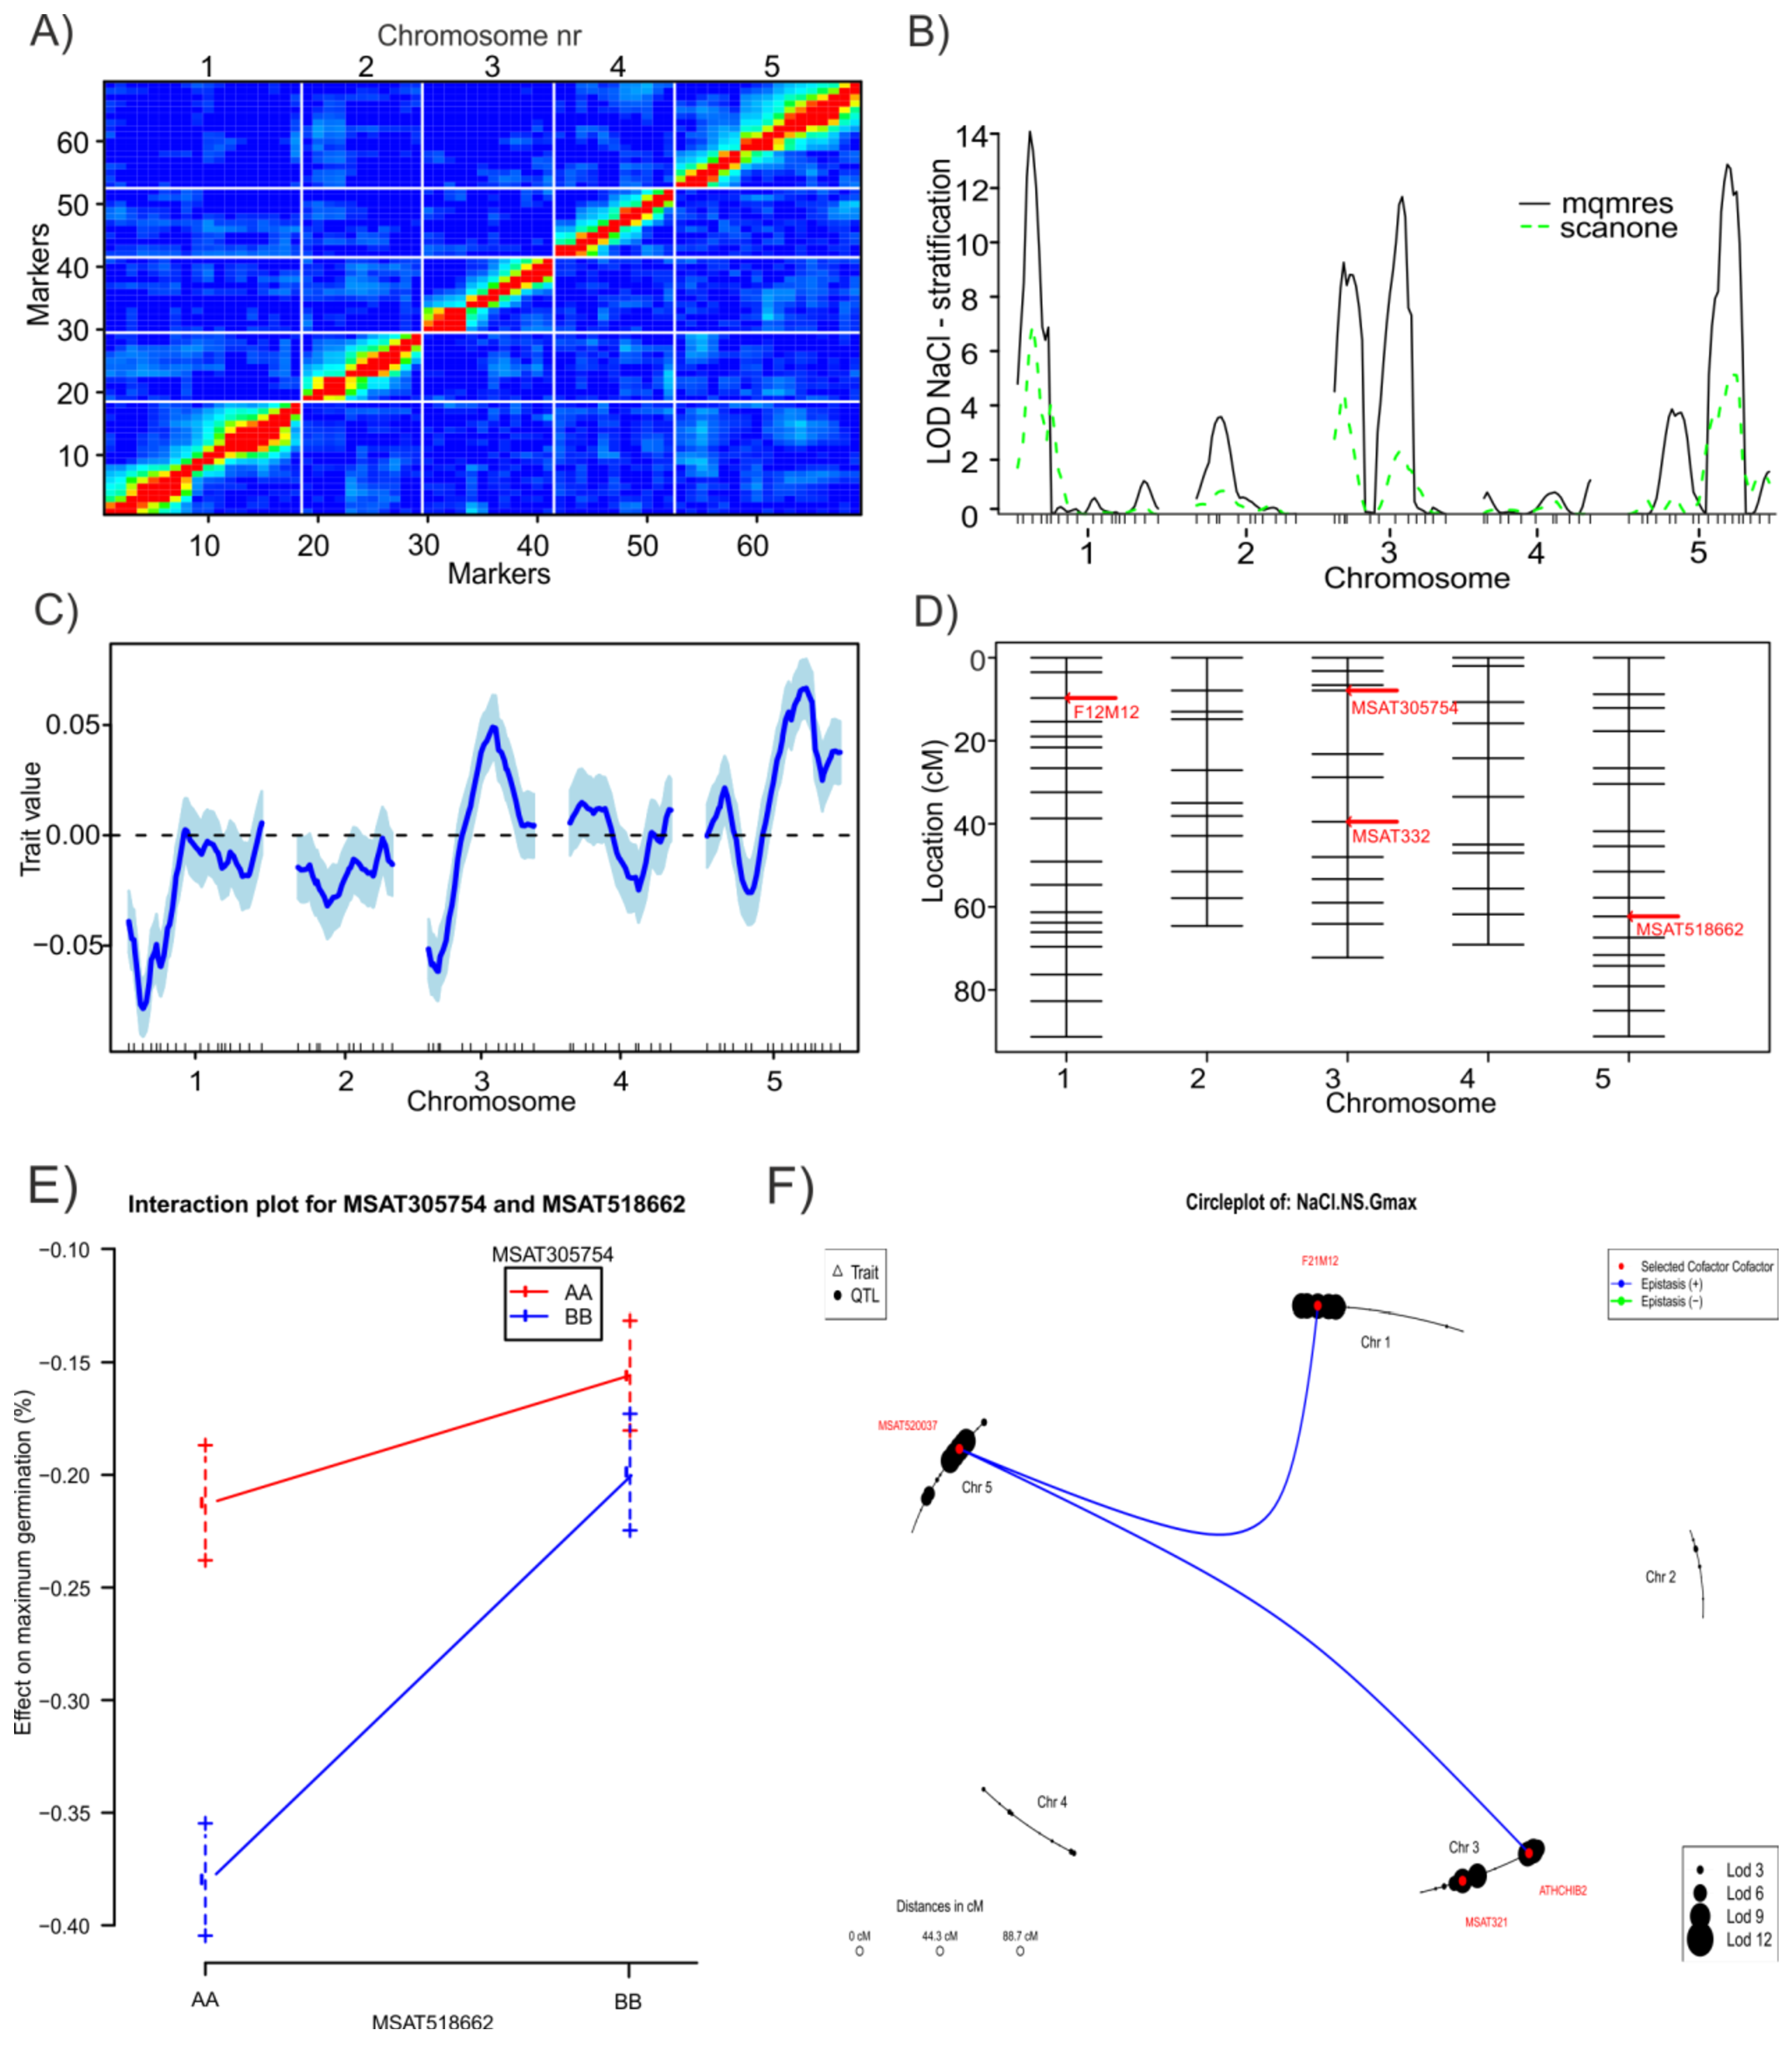
\includegraphics[keepaspectratio,scale=0.30]{eps/image_3_1_2.eps}
  \caption[Generated Output.]{R/QTL output for the effect of 100mM NaCl on the maximum germination without 
          stratification. A) Pairwise recombination fractions; B) Phenotype distribution histogram without 
          normalization ; B) LOD profile comparison between MQM and Haley-Knott (scan-one) interval mapping; 
          C) Genome wide additive effect based on raw phenotype data D) Genetic map showing the significant 
          QTL markers; E) Interaction plot showing the effect size comparison between marker MSAT305754 and 
          MSAT518662 at the Sha (AA) and Bay-0 (BB) alleles; F) Circle plot showing interactions between 
          all significant markers.}
          \label{fig:generatedoutput}
\end{figure}

Analysis of natural variation that is captured in well-defined recombinant inbred populations has 
shown to be a powerful tool to detect important loci that influence the traits under study 
\cite{Alonso-Blanco:2009}. To uncover the loci with genetic variation a statistical framework is 
needed. For this, any programming language can be used which supports statistics. In the life sciences 
the statistical language R is often the prime candidate. R is open source, contains the latest in 
statistical analysis methods and has a large community for help and support (\url{http://www.r-project.org/}). 
Furthermore, it has the R/qtl package \cite{Broman:2003}, which contains an array of different 
QTL mapping methods, including Single Marker Mapping, Interval Mapping and Multiple QTL Mapping (MQM) 
\cite{Arends:2010}. Although all possibilities to perform a detailed QTL analysis including data 
preprocessing and output formatting are present in R, it requires extensive knowledge of the R-syntax 
to combine all necessary steps in a single analysis protocol that can loop through hundreds or 
thousands of traits. 

We present a script that can perform these tasks. This type of automated analysis combined with 
efficient data visualization is a necessary step to keep up with the increasing rate of biological 
data production. For using single trait mapping the effect of a certain treatment, e.g. germination 
at high temperature, must be corrected by the germination characteristics under control conditions. 
Here, we subtracted the observed germination under stress conditions from values for germination 
under control conditions. This correction can lead to complicated interpretation, especially when the 
environment under study affects loci with already strong effects under control conditions. Further, 
it can reduce statistical power due to summation of the error components. Therefore we performed an 
additional analysis using a QTL by environment (QTLxE) approach \cite{Vargas:2006, Moreau:2004}. 
Instead of considering individual responses, one can then treat the stress conditions as a set of 
environmental perturbations and evaluate a single trait (such as germination percentage). Because 
several environments are taken into account simultaneously, the statistical power to detect loci 
that are affected by several environments increases and interpretation becomes more intuitive as the 
need for correcting the stress response by the control response is eliminated \cite{Boer:2007}.

The Bay-0 x Sha RIL population consists of 420 lines that were genotyped in the F6. This relatively 
low degree of inbreeding provoked residual heterozygosity present at almost all genome positions. 
This residual heterozygosity can be used to confirm QTL positions, as it provides a possibility to 
study both parental alleles at the locus of interest in an elsewhere homozygous background. 
In contrast to conventional near isogenic lines (NILs) the genetic background of heterogeneous 
inbred lines (HIFs) consist of a mix of the two parental genomes. The availability of a genome wide 
set of HIF lines for the Bay-0 x Sha RIL population provides a fast and accurate means to confirm 
detected QTL loci.

\subsection{Results}

\subsubsection{Single trait QTL mapping}
To evaluate the response of germination to a certain treatment, we first subtracted the observed 
germination at test conditions from germination at the proper control conditions. For example, the 
effect of NaCl on germination after cold stratification is determined by subtracting Gmax on 
NaCl from Gmax on water. This subtraction was reversed for the rate and uniformity parameters to 
correct the reversed nature of these parameters (e.g. slower germination results in a larger t10 
and t50). Table \ref{table:codes} gives an overview of all corrections that have been applied. 

\begin{figure}[!ht]
  \centering
  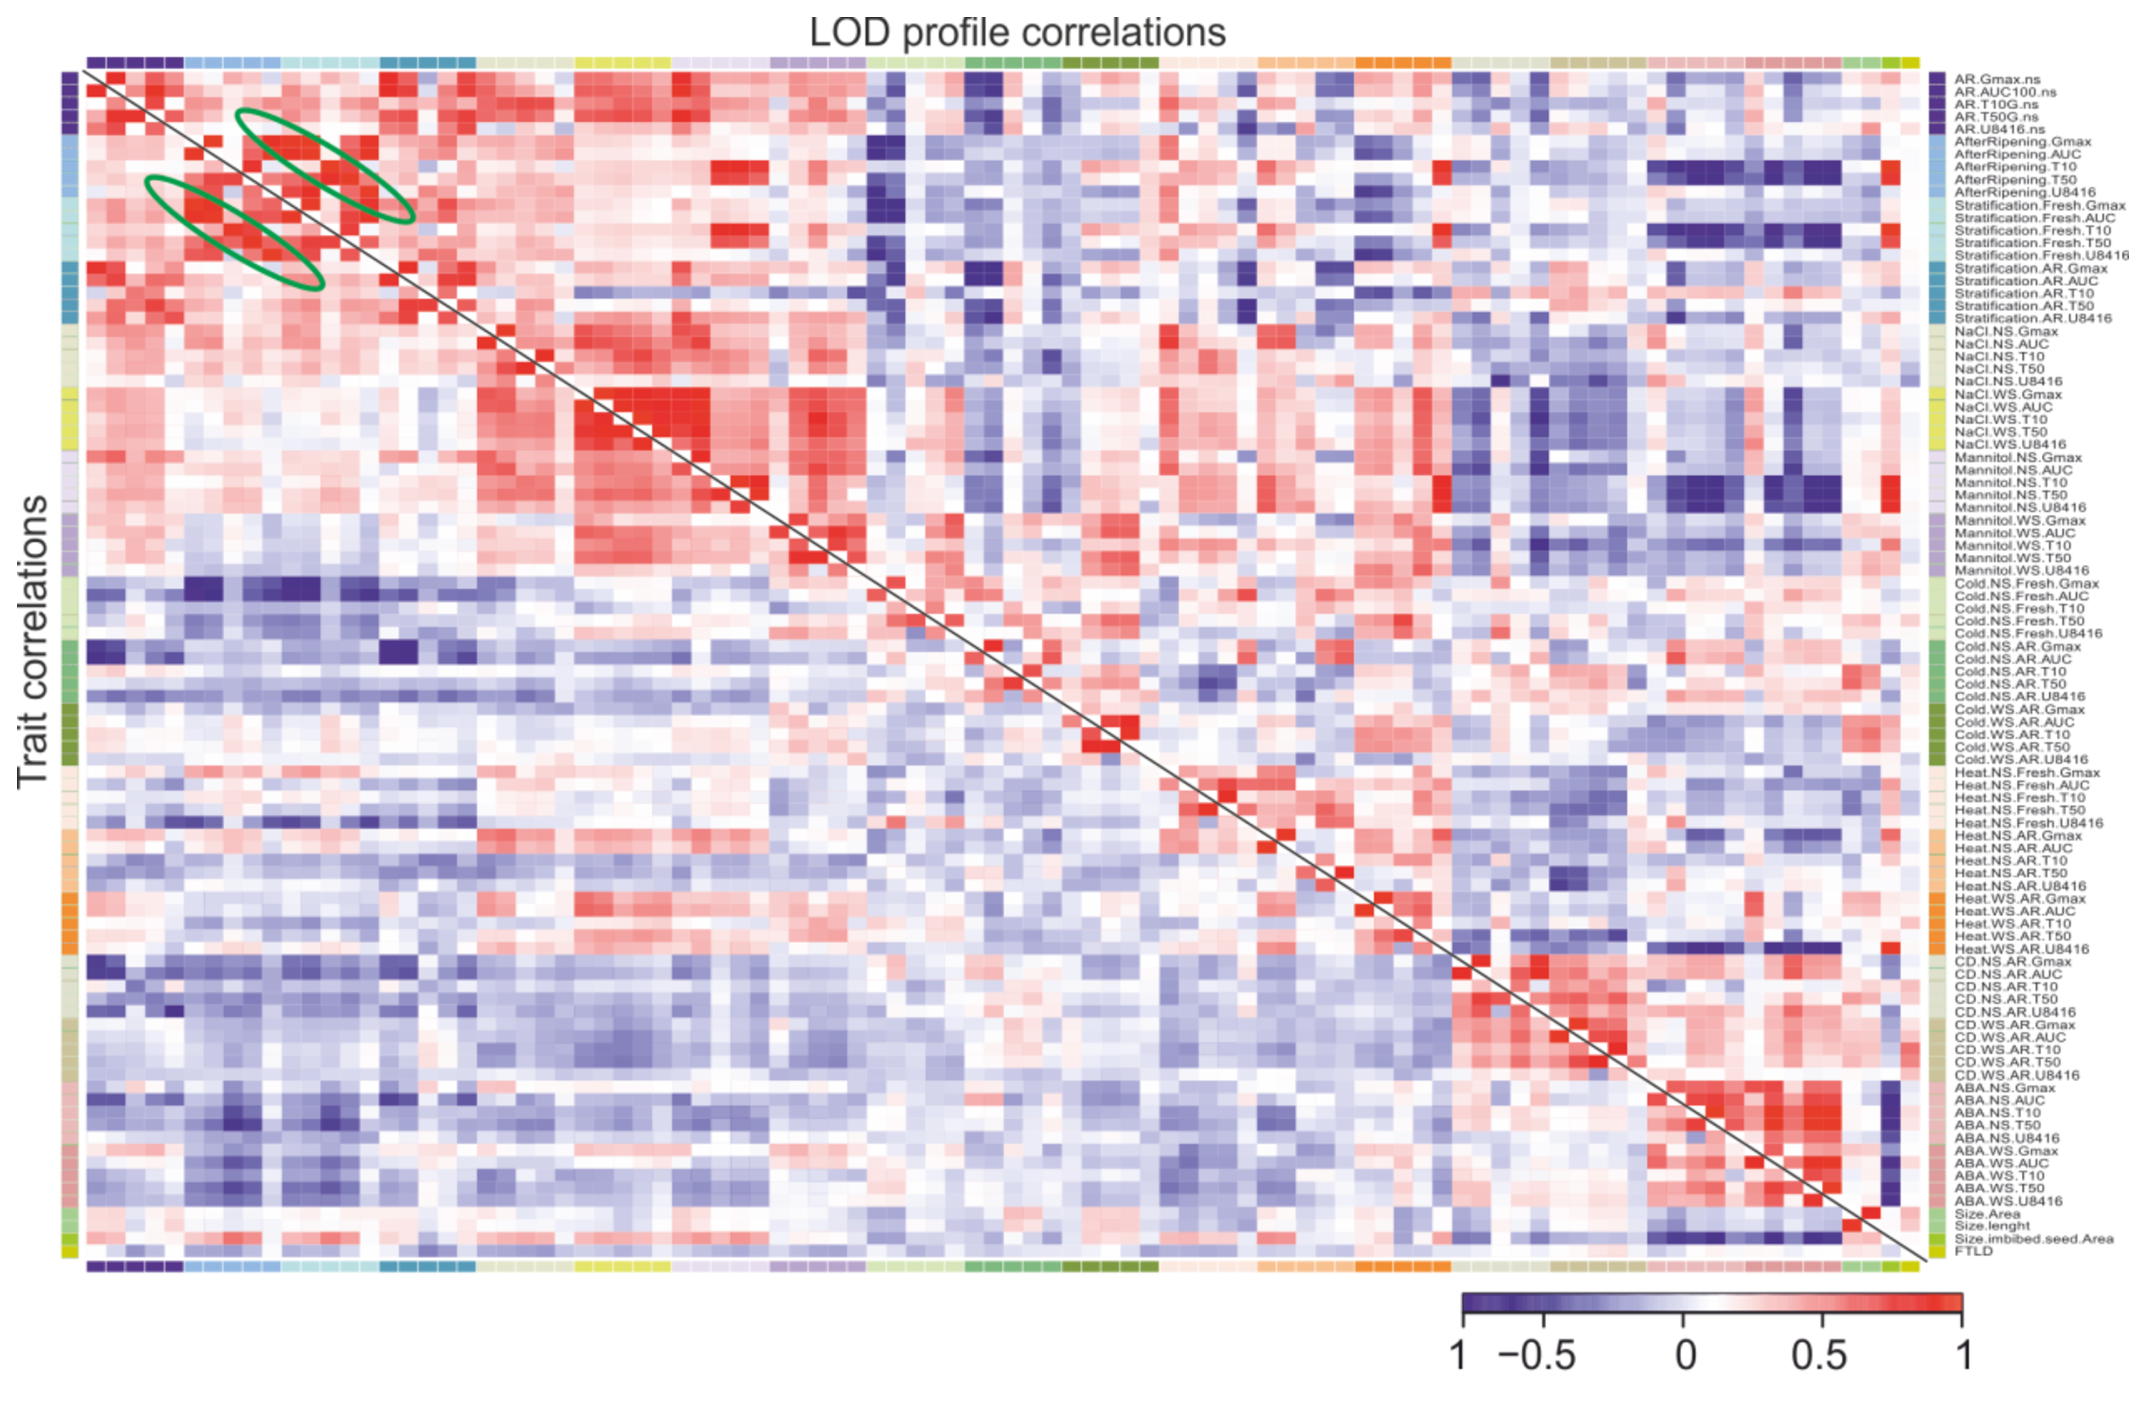
\includegraphics[keepaspectratio,scale=0.30]{eps/image_3_1_3.eps}
  \caption[Heatmap of correlation.]{Correlation between all trait values (bottom left panel) and between 
          all LOD profiles (top right panel). Traits are indicated by the color code depicted in Table \ref{table:codes}. 
          Green circles indicate an example of the close correlation between "after-ripened" and "fresh 
          with stratification" trait values.}
\end{figure}

An analytical protocol was designed, using the popular R/qtl package of R to analyze trait data of 
recombinant inbred populations with the multiple QTL model approach \cite{Arends:2010}. When 
performing a detailed QTL analysis it is important that several steps are performed or checked. 
Missing genotypic data is imputed and a recombination frequency plot is generated (Fig. \ref{fig:generatedoutput}A). In 
the next step, quality of the trait data is investigated. Outliers are detected and removed using 
a Z-score transformation with a user defined threshold. As an extra control the results of MQM mapping 
were always compared to standard interval mapping, using the parametric model with Haley Knott 
regression \cite{Haley:1992} (Fig. \ref{fig:generatedoutput}B). The whole genome additive effect was estimated based 
on the non-transformed data as half the difference between the phenotypic averages for the two 
homozygotes (Fig. \ref{fig:generatedoutput}C).

R/qtl MQM uses a backward elimination of cofactors. As a rule of thumb one can select a maximum of 
$N-20$ initial cofactors with this procedure \cite{Handbook:Jansen:2007}, with $N$ being the number of lines in 
the RIL population. In our script, a cofactor file can be provided with the selection of the initial 
cofactors. When no cofactors are provided, the analysis will be performed without cofactors resulting 
in an analysis comparable with the composite interval mapping (CIM) method. For the analysis of the 
Bay-0 x Sha population we pre-selected 39 out of 69 markers as possible cofactors. Cofactors were selected 
based on their quality (least amount of missing data or heterozygous status) and physical cM position, 
attempting to obtain intervals of about 10 cM. Although the procedure allows the selection of all 69 
markers as cofactors, this does not improve mapping and only lowers statistical power due to the 
multiple testing correction in the permutation analysis. The provided cofactor file is used to perform 
automated backward elimination of cofactors.

\begin{figure}[!ht]
  \centering
  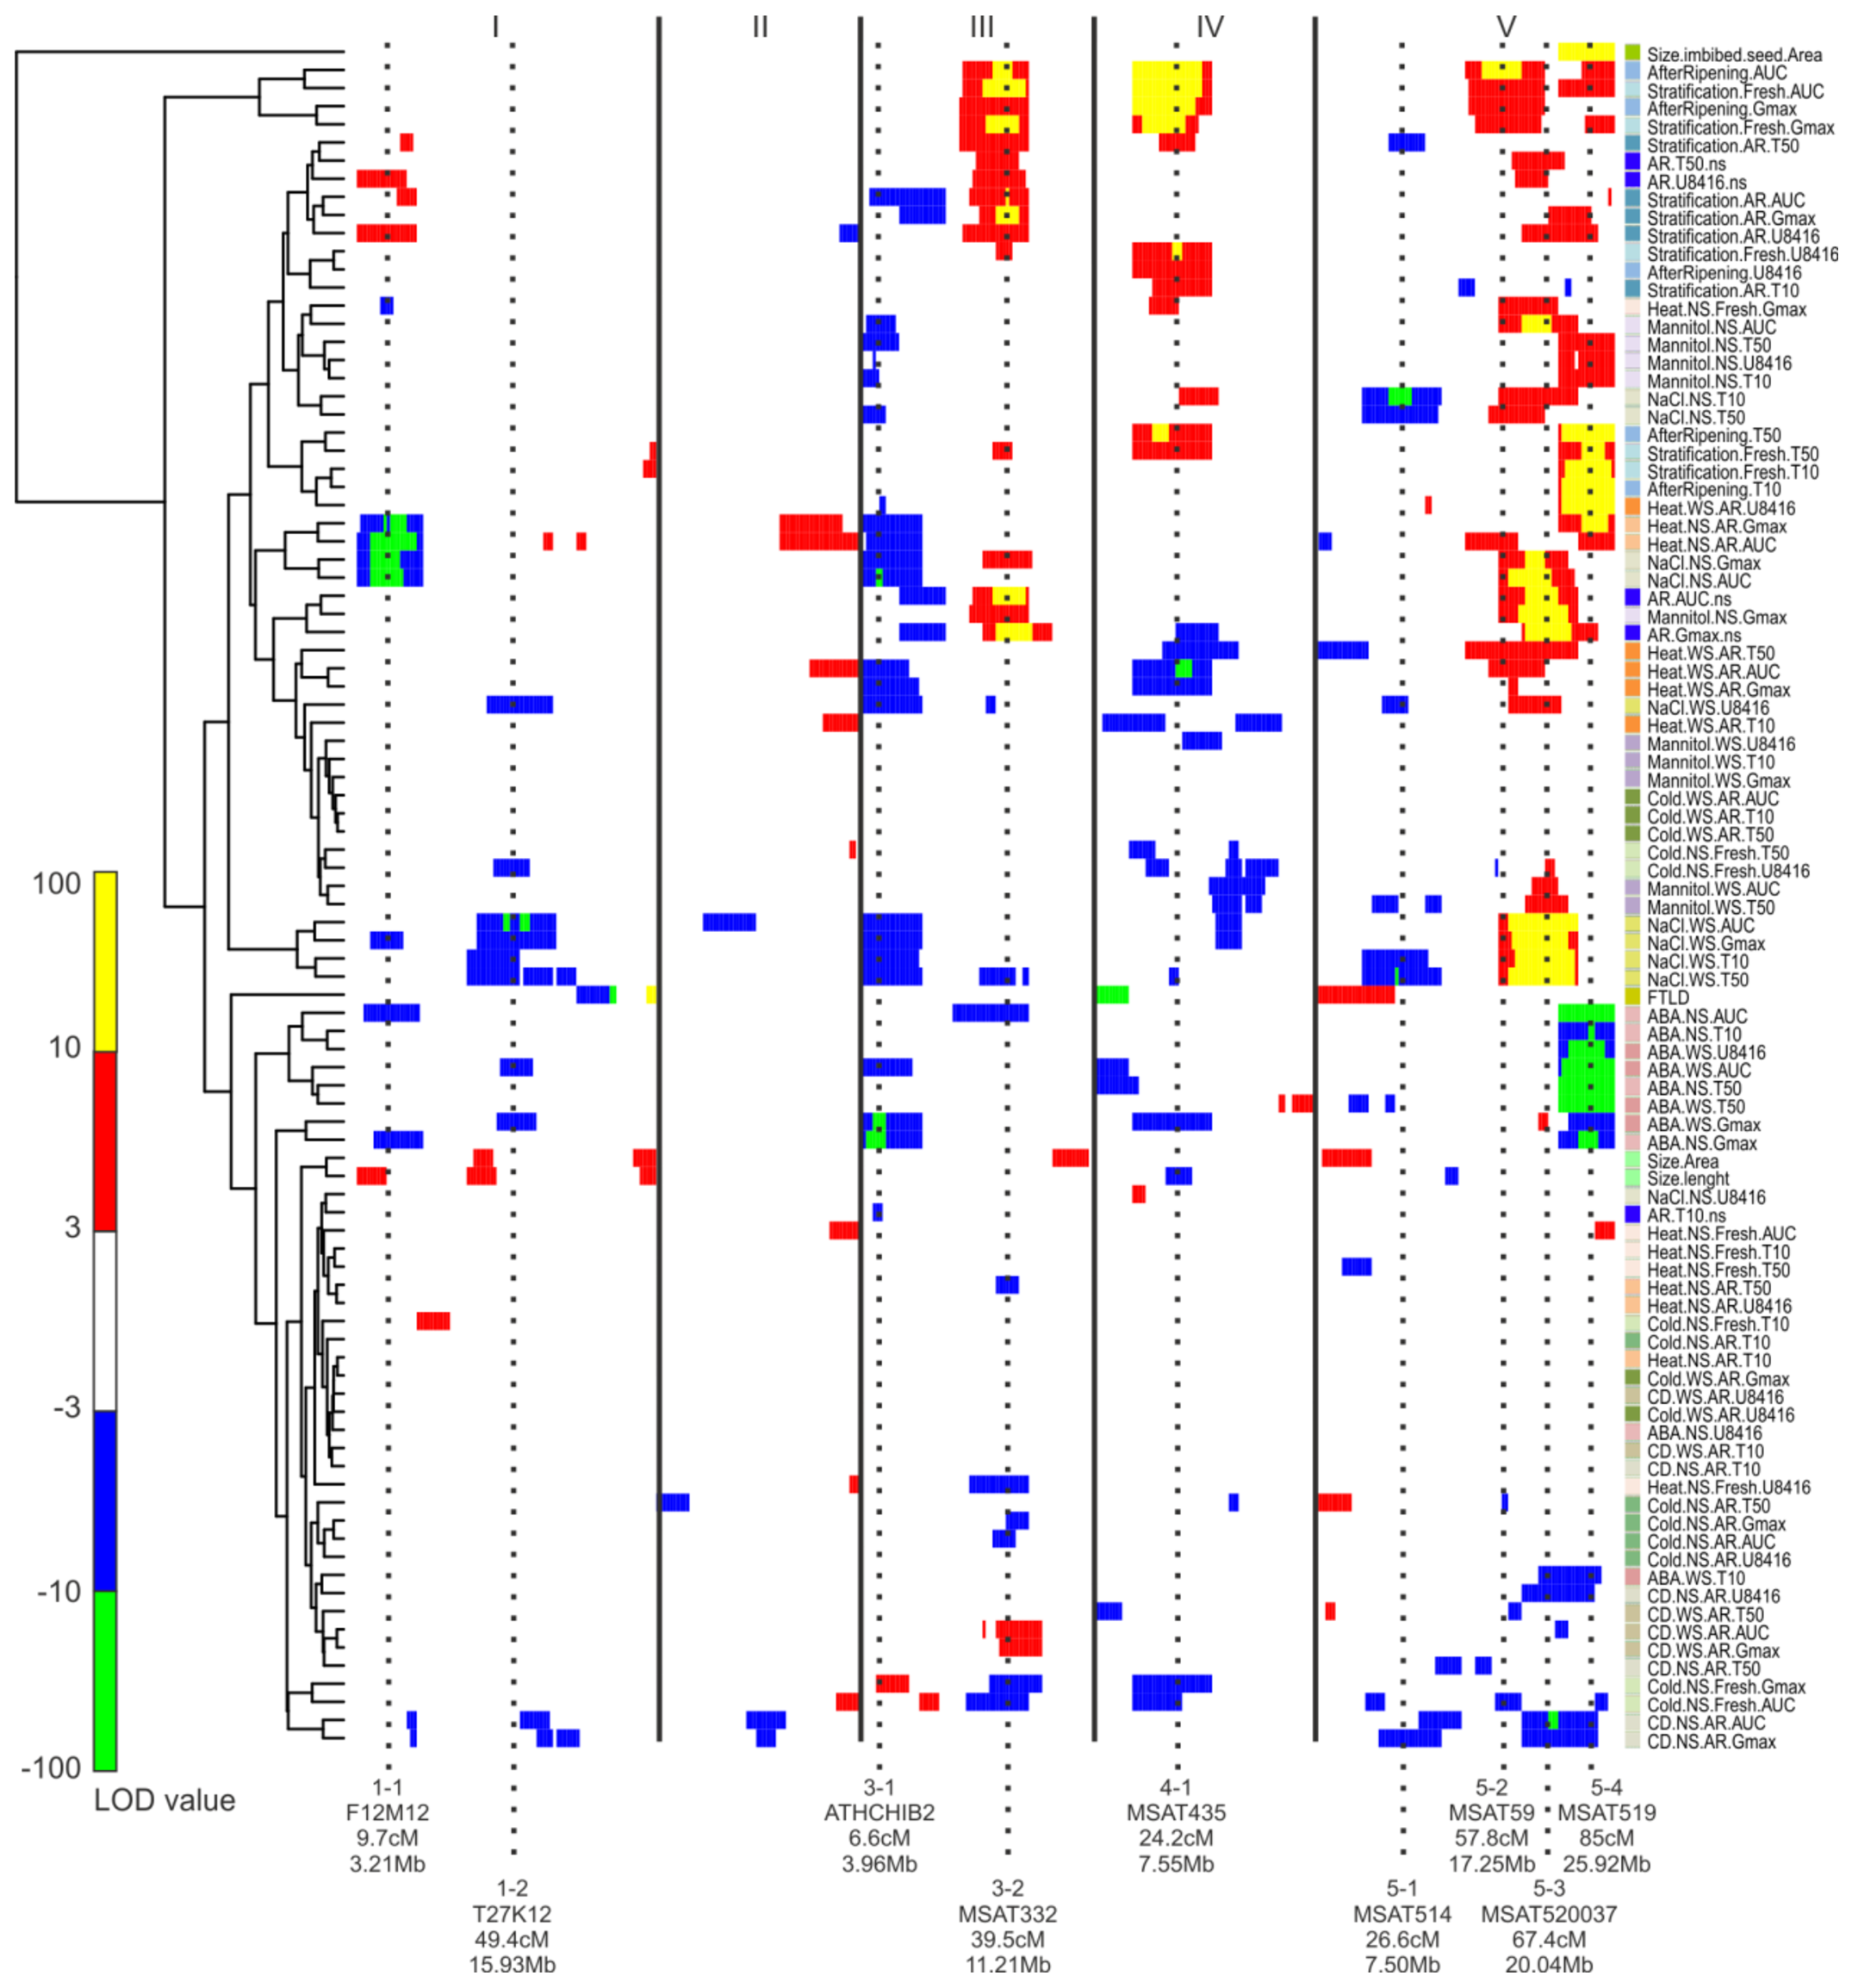
\includegraphics[keepaspectratio,scale=0.30]{eps/image_3_1_4.eps}
  \caption[QTL locations.]{A clustered heat map showing the LOD profiles of the measured traits is automatically 
          produced. Columns indicate chromosome position along the 5 chromosomes; rows indicate individual trait 
          LOD profiles. A false color scale is used to indicate the QTL significance. Positive values (yellow and red) 
          represent a larger effect of the treatment in Shahdara, negative values (blue and green) in Bayreuth..}
\end{figure}

Backward elimination is performed to remove cofactors that do not significantly contribute to the fit 
of the initial model. This is achieved by comparing Akaike's information criterions (AIC) of the 
different models \cite{Jansen:1993}. Using the final selected QTL model, the mapping LOD scores are 
calculated for all genetic markers. Plots showing all significant markers are produced automatically 
(Fig. \ref{fig:generatedoutput}D). We have used the procedure described to map all 327 individual measurements but to enhance
readability we only show average values for each trait (94 traits)

\subsubsection{QTLxQTL Interactions}
Epistatic interactions between QTL can help to elucidate meaningful co-localizations and will enable an 
efficient design of follow up experiments. Besides the visualization of the epistatic interactions per 
trait (Fig. \ref{fig:generatedoutput}F) our script creates an output that can help to visualize all detected epistatic 
interactions in a single plot. This output file in sif format summarizes all detected epistatic 
interactions (Fig. \ref{fig:epistaticinteractions}). Among others, clear hotspots of 
epistatic interactions between QTL loci on chromosome 3, 4 and 5 (resp. ATHCHIB2 + MSAT332, MSAT435 and 
MSAT520037 + MSAT519) were observed for germination on salt (yellow lines) and dormancy (blue lines). 
Next to the importance of detecting possible interacting loci this QTLxQTL analysis provides additional 
arguments for co-locating QTL to be of similar genetic origin. Overall, the creation of this type of 
summarizing figures is greatly facilitating the interpretation of large datasets.

\begin{figure}[!ht]
  \centering
  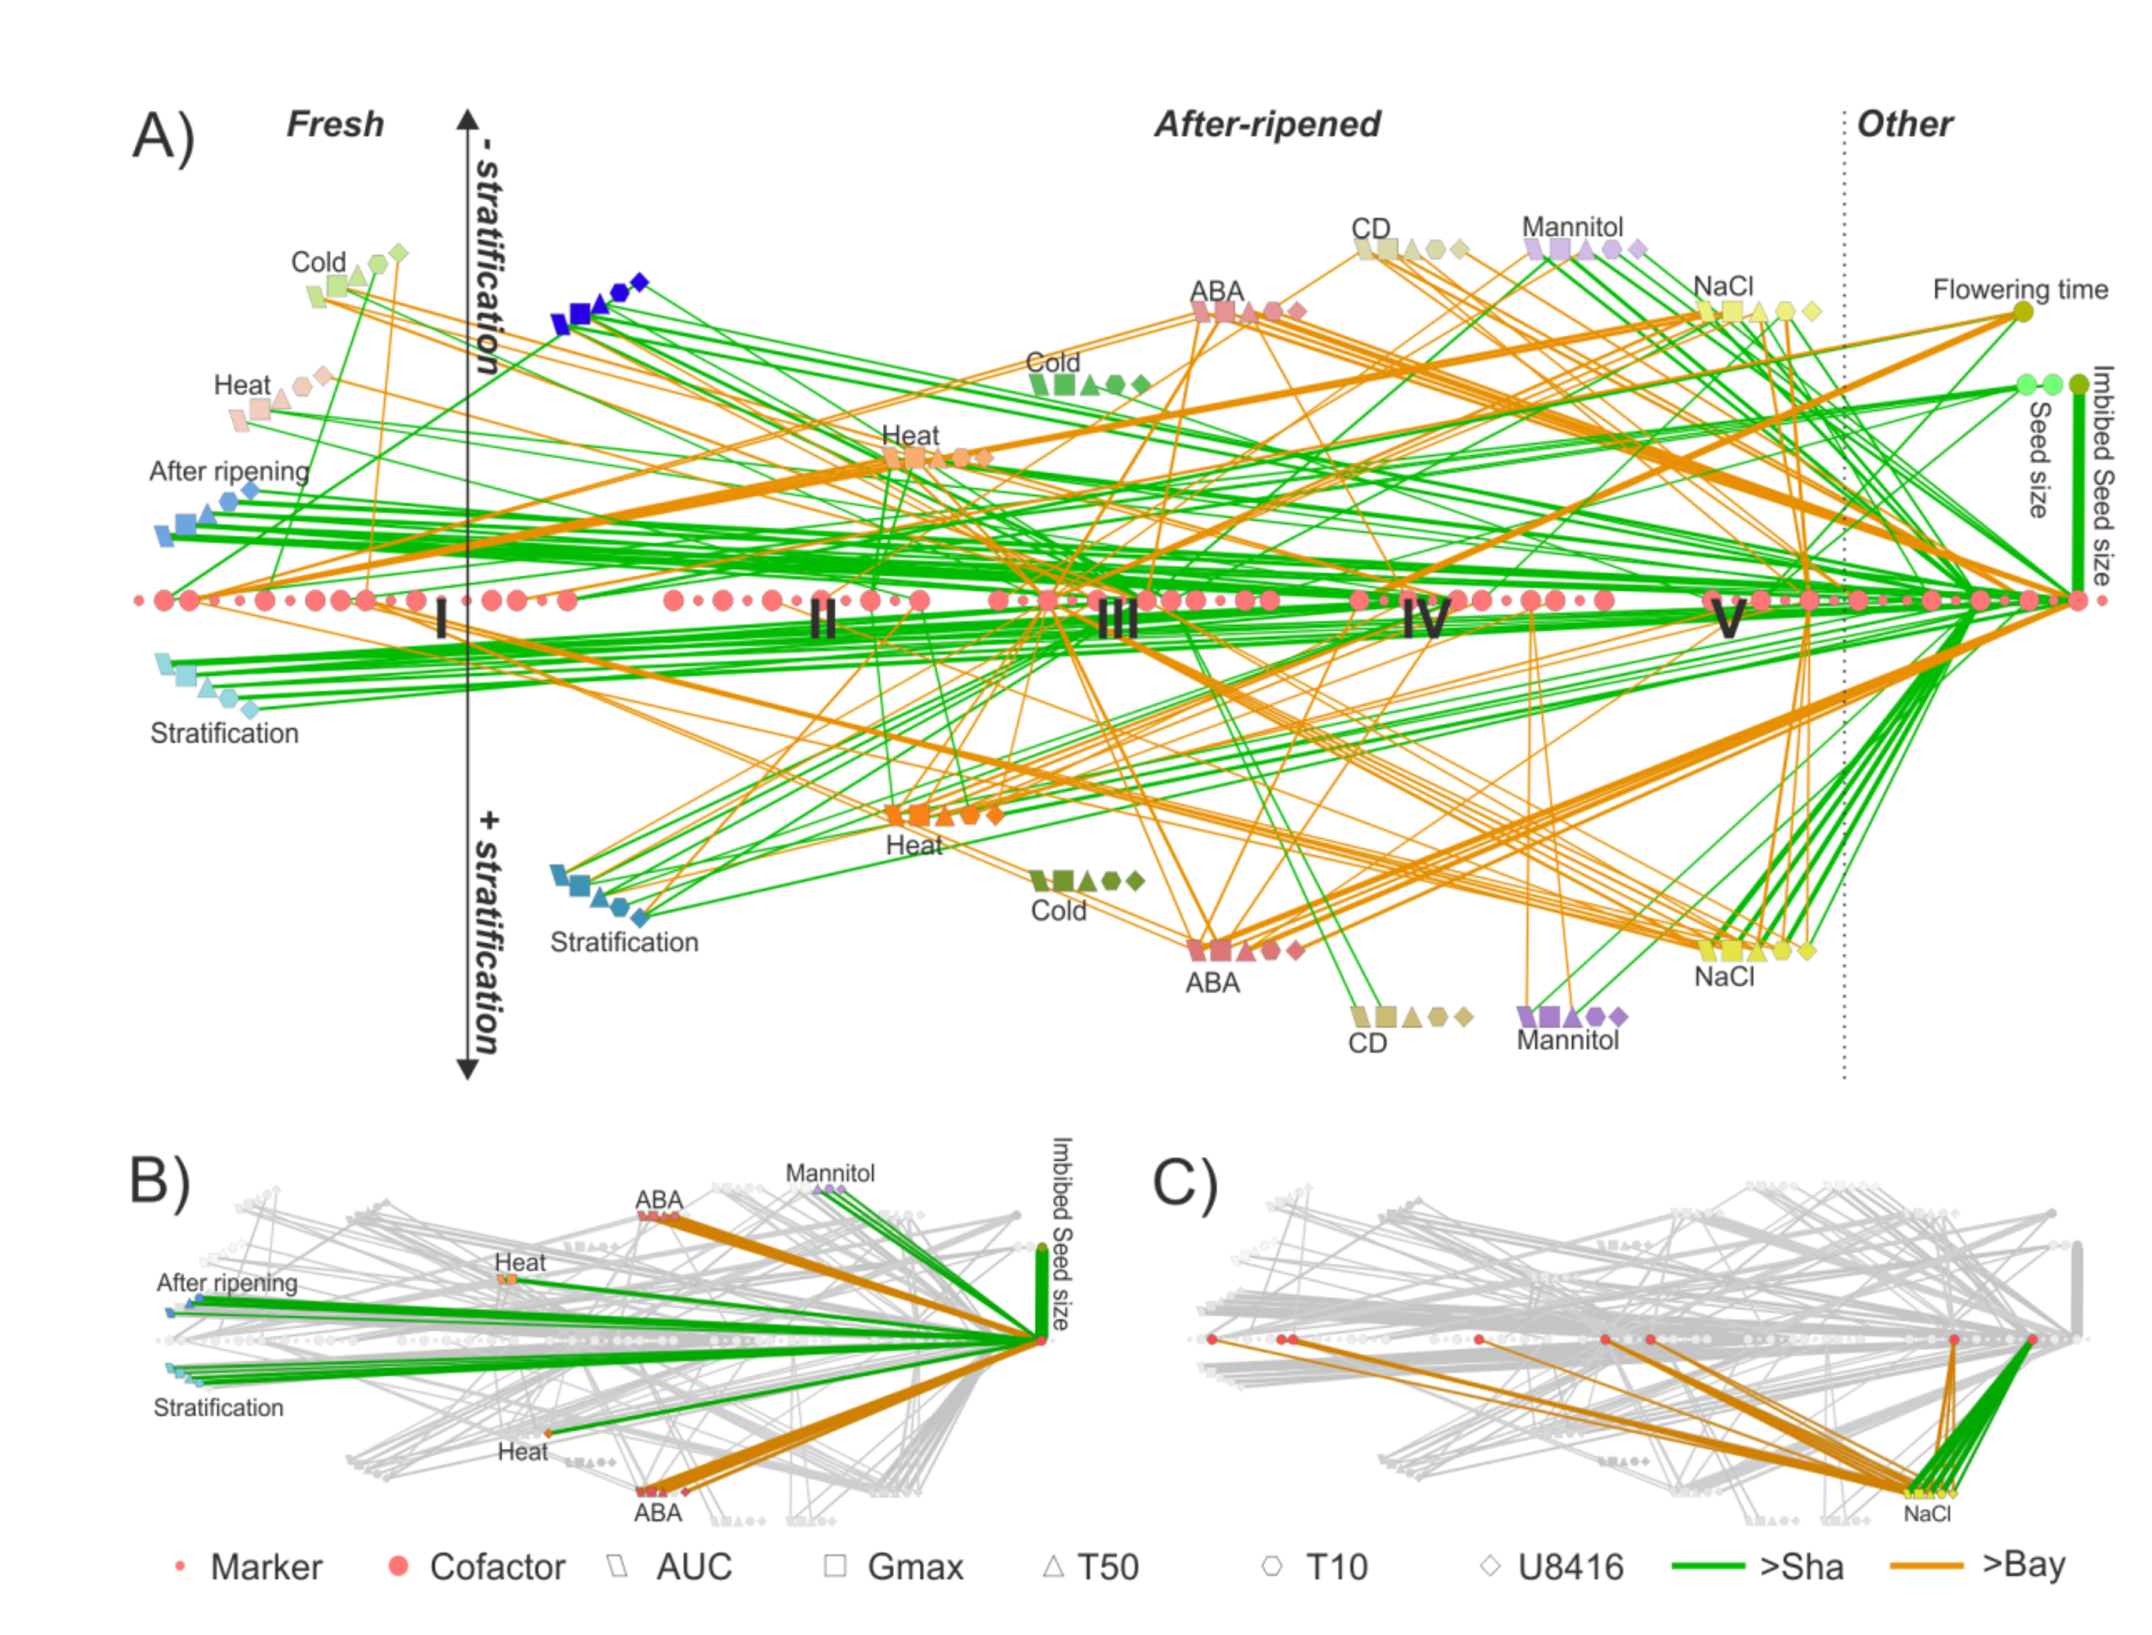
\includegraphics[keepaspectratio,scale=0.30]{eps/image_3_1_5.eps}
  \caption[Cytoscape marker trait network.]{Cytoscape Marker-Trait network. A) Significant QTL positions are 
          indicated by a connection between traits and markers, edge colors indicate the direction of the QTL 
          effect, line width indicates the LOD score; B) Sub- network showing all traits with a significant 
          QTL at marker MSAT519; C) Sub- network showing all markers with significant QTL for germination on 
          NaCl with stratification.}
\end{figure}

\begin{figure}[!ht]
  \centering
  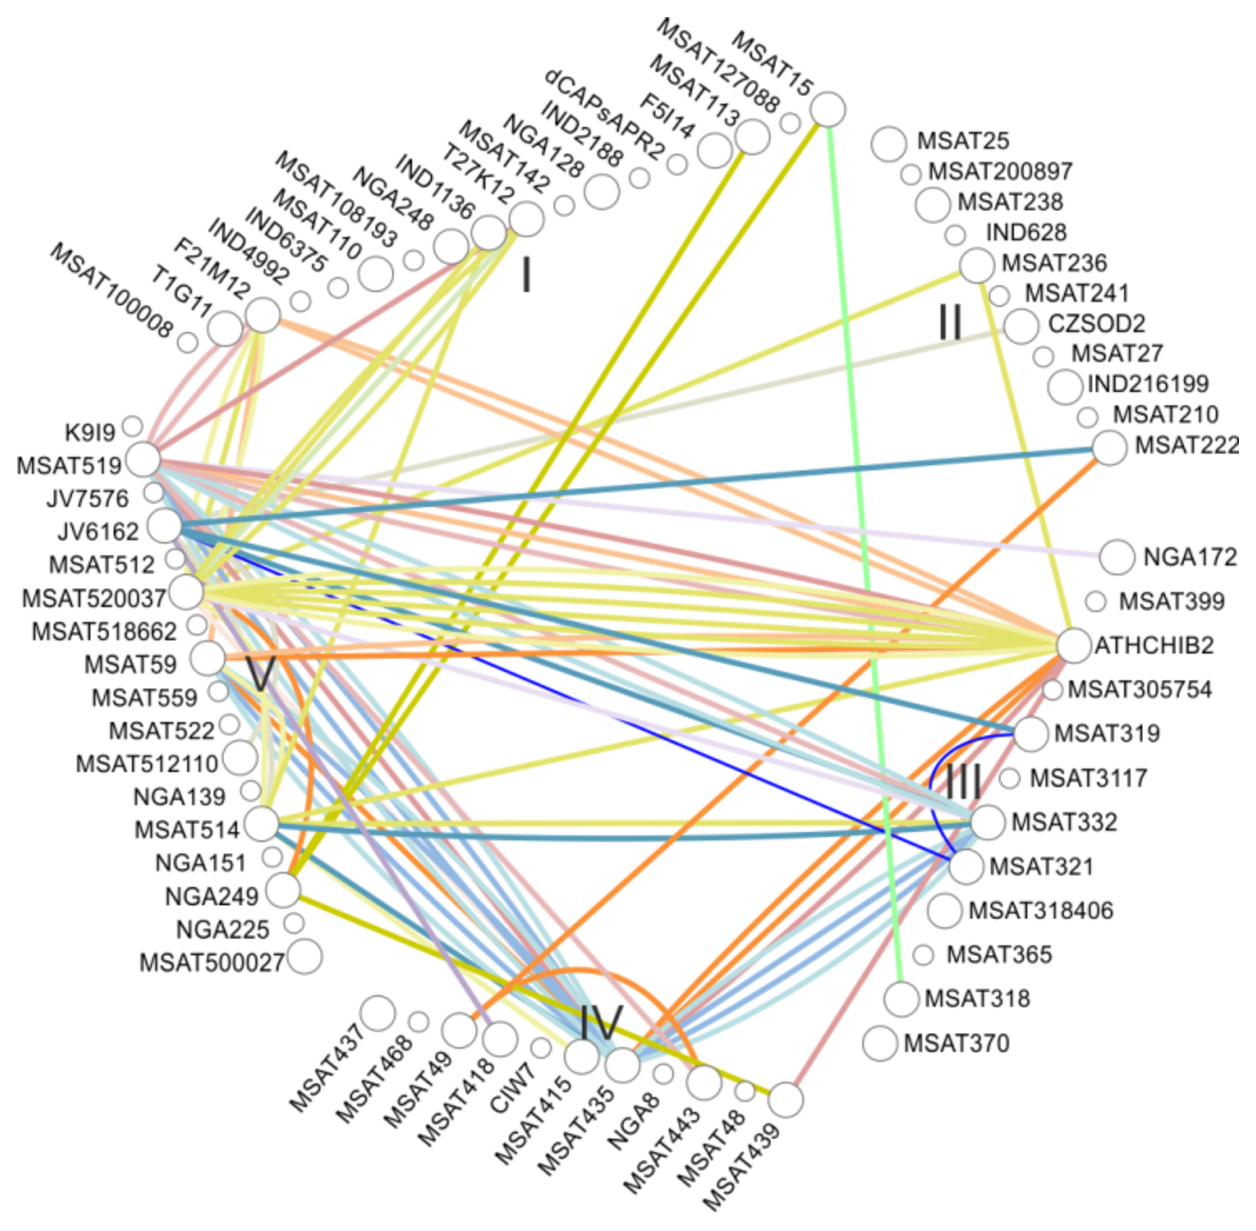
\includegraphics[keepaspectratio,scale=0.30]{eps/image_3_1_6.eps}
  \caption[Epistatic interaction network.]{Epistatic interaction network created with Cytoscape from the 
          interaction.sif output file. Nodes indicate markers (small circles) and selected cofactors (large 
          circles). Edges represent the detected significant epistatic interactions (edge colors represent 
          traits, see table \ref{table:codes} for colors).}
          \label{fig:epistaticinteractions}
\end{figure}

\subsubsection{QTLxEnvironment interaction}
To obtain a parameter for the response, we had to correct all values with their proper control condition 
values. This sometimes led to complex interpretation, which can be circumvented by using the non-corrected 
germination parameters and model them over the various environmental conditions that were tested. Because 
several environments are taken into account simultaneously the statistical power to detect loci that are 
affected by several environments increases and interpretation becomes more intuitive as the need for 
correcting the stress response by the control response is eliminated. By using this approach the 
sensitivity of a specific QTL for environmental conditions can be determined for each separate germination 
parameter. Details about the procedure are described in Material and Methods. Results are summarized in 
figure \ref{fig:gegenomewide}. The final model P-value profiles (top panel, Fig. \ref{fig:gegenomewide}) clearly show the great consistency 
between the 5 germination parameters that we measured. However, a closer look also reveals loci that 
are affecting different germination curve parameters. For example, the QTL on top chromosome 5 is not 
detected by measuring maximum germination but is well defined when using $t_{50}$ or $t_{10}$ as parameter. As 
expected, the parameter AUC (Area Under the Curve) is outperforming the others as it represents a 
combined value for maximum germination percentage, rate and uniformity. For comparison of the 
environment-specific QTL effects for the 5 different germination parameters (5 lower panels, Fig. \ref{fig:gegenomewide}) 
the effects could be compared with germination under control conditions. For example, after ripened 
seeds without stratification (AR.NS) can guide as reference for the stress treatments (AR.NS.ABA, AR.NS.CD, 
AR.NS.Cold, AR.NS.Heat, AR.NS.Mannitol, AR.NS.NaCl). The same analogy holds true for after ripened seeds
without stratification (AR.NS) and freshly harvested seeds without stratification (Fresh.NS). In this way 
stress specific QTLs on chromosome II and top chromosome III can easily be identified. Interestingly, some 
QTLs, including germination at low temperature (top chromosome I) and germination in the presence of 
exogenous ABA (bottom chromosome V) displayed opposite effects on germination when compared to the 
other treatments.

\begin{figure}[!ht]
  \centering
  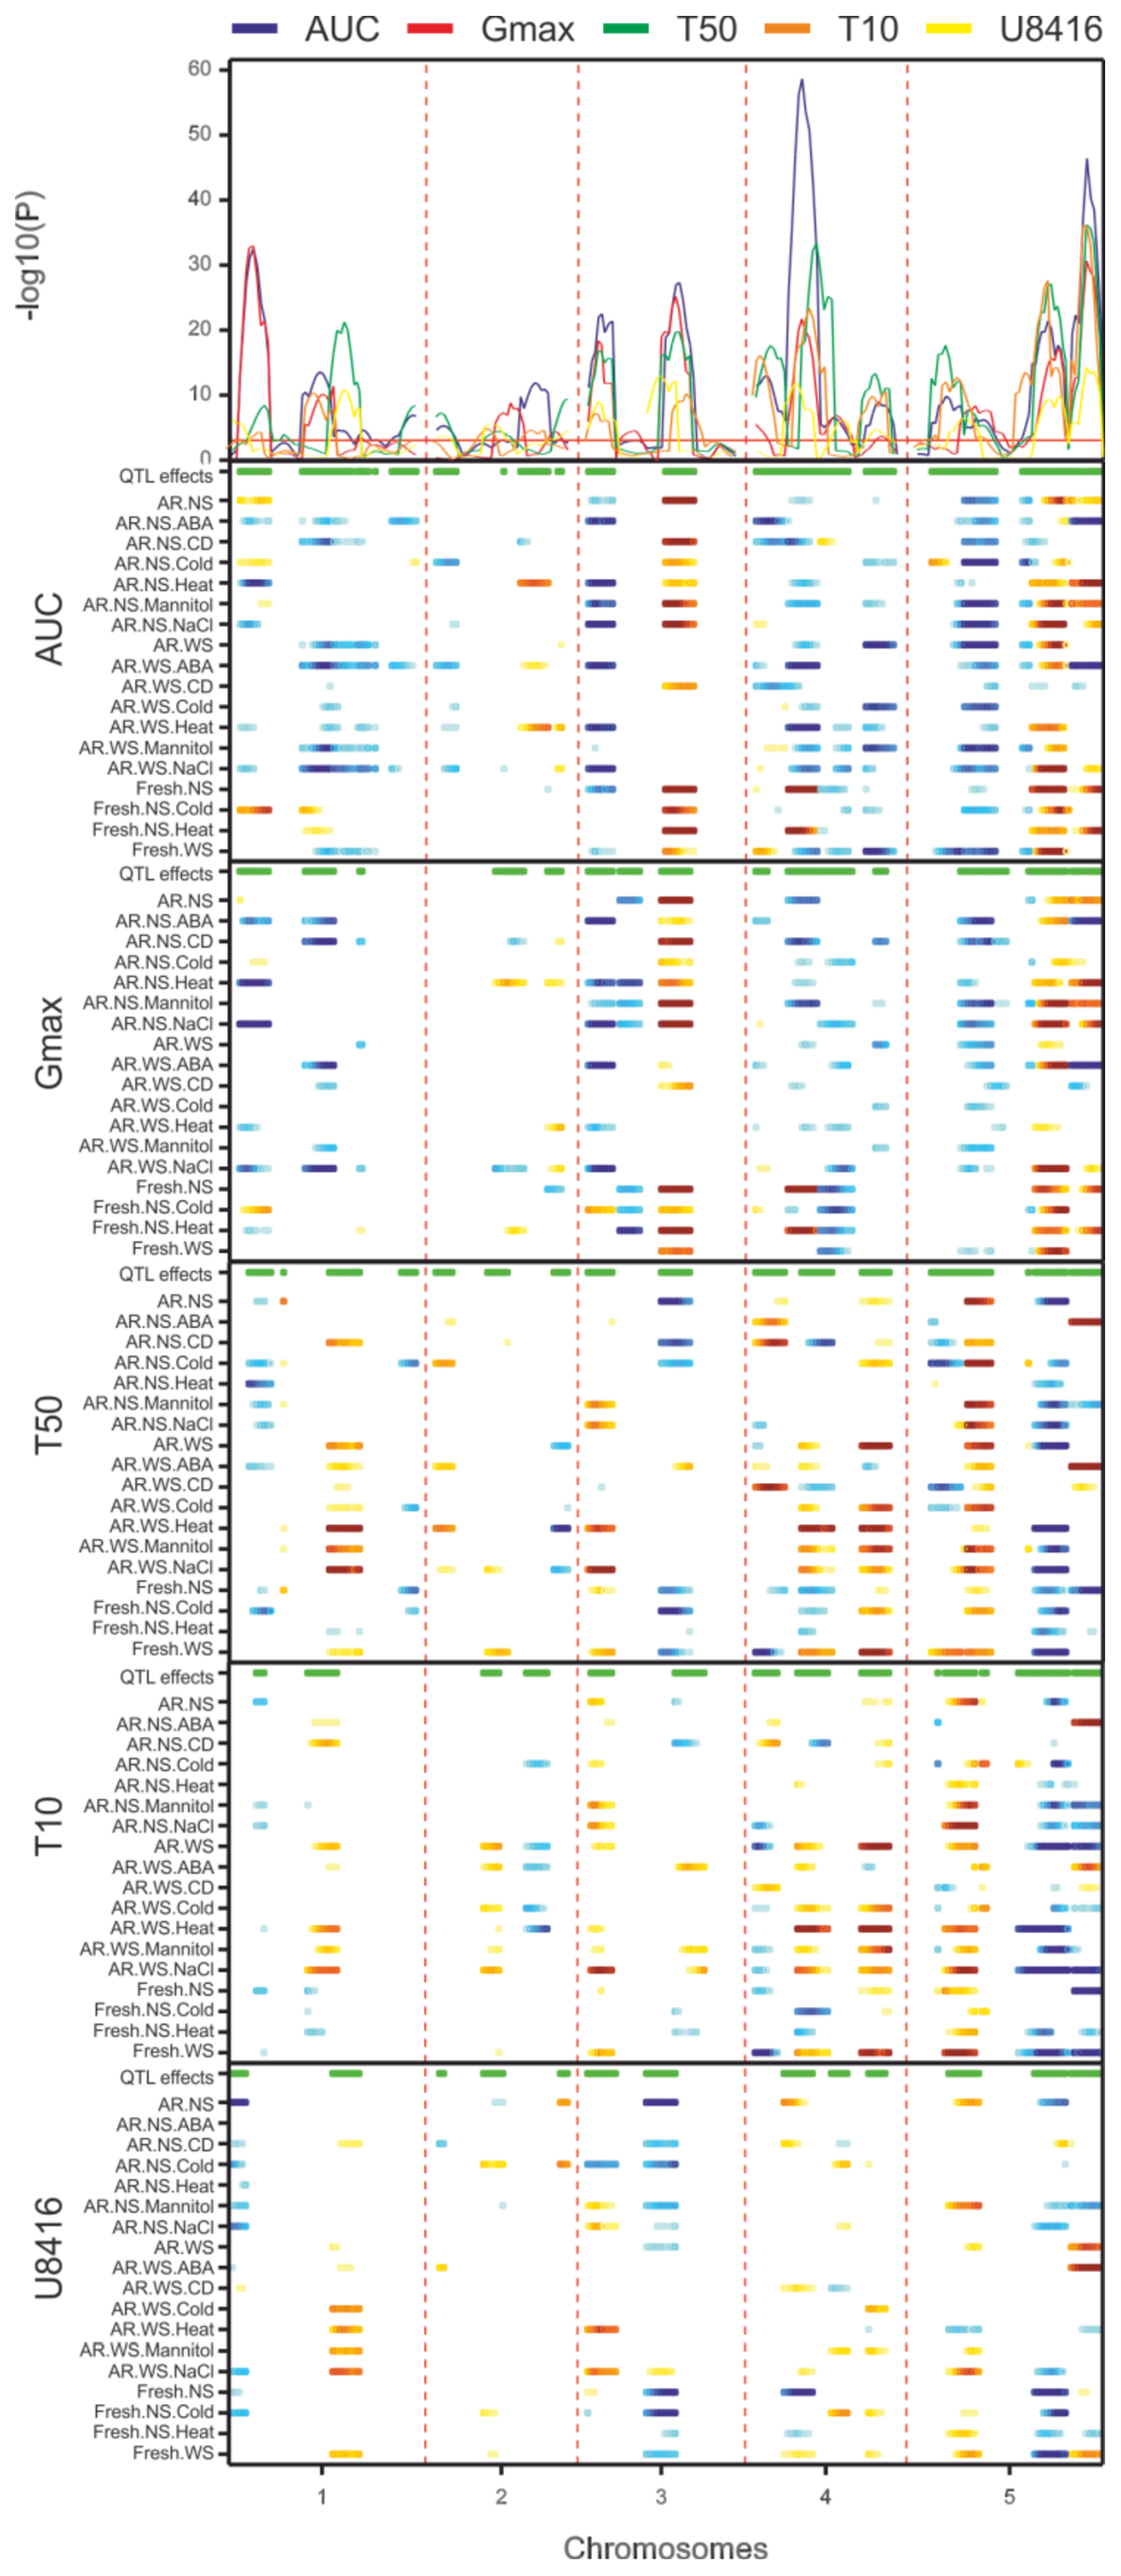
\includegraphics[keepaspectratio,scale=0.20]{eps/image_3_1_7.eps}
  \caption[G:E genome wide QTL scan.]{Genome scan for QTLxEnvironment effects for seed germination. The P-values for 
          the main effects of the different germination parameters are shown in the top panel. The red horizontal line 
          is the genome wide significance threshold. The 5 bottom panels show the environment specific QTL effects. 
          The green line indicates significant environment specific effects. For both Gmax and AUC a bigger effect of 
          the Sha allele is indicated in yellow-red (Bay-0 in cyan-blue). The color scale is opposite for the t50, 
          t10 and U8416 parameters due to the inverted nature of these parameters.}
          \label{fig:gegenomewide}
\end{figure}

\subsubsection{QTL confirmation}
Taking advantage of the residual heterozygosity present in the F6 generation of the Bay-0 x Sha population, 
combined with the large population size, we were able to confirm several QTL following the heterogeneous 
inbred family (HIF) approach. In short, RIL lines which are heterozygous at the locus of interest were 
selected in the next generation for lines homozygous for both parental alleles. These 'families' are 
near isogenic lines (NIL) which can be used to confirm the observed allelic effects (Fig. \ref{fig:confirmation}A). We 
applied this strategy for 7 of the major QTL that we detected in  this study and tested the 5 germination 
parameters for 11 different conditions. For a single parameter (Gmax) and a single HIF (line HIF103) the 
analytical procedure is summarized in figure \ref{fig:confirmation}B. We 
detected a vast QTL for imbibed seed size at the bottom of chromosome 5, which could be confirmed by the 
use of HIF103. Upon imbibition seeds swell due to rapid water uptake and possibly because of the 
expansion of the inner mucilage layer. In Sha, which is a natural mutant for the MUM2 gene 
\cite{Macquet:2007}, this swelling did not occur. Also the HIF lines at the MUM2 position showed a 
clear difference in swelling phenotype which was still significant 24 hours after imbibition (Fig. \ref{fig:swelling}).

\begin{figure}[!ht]
  \centering
  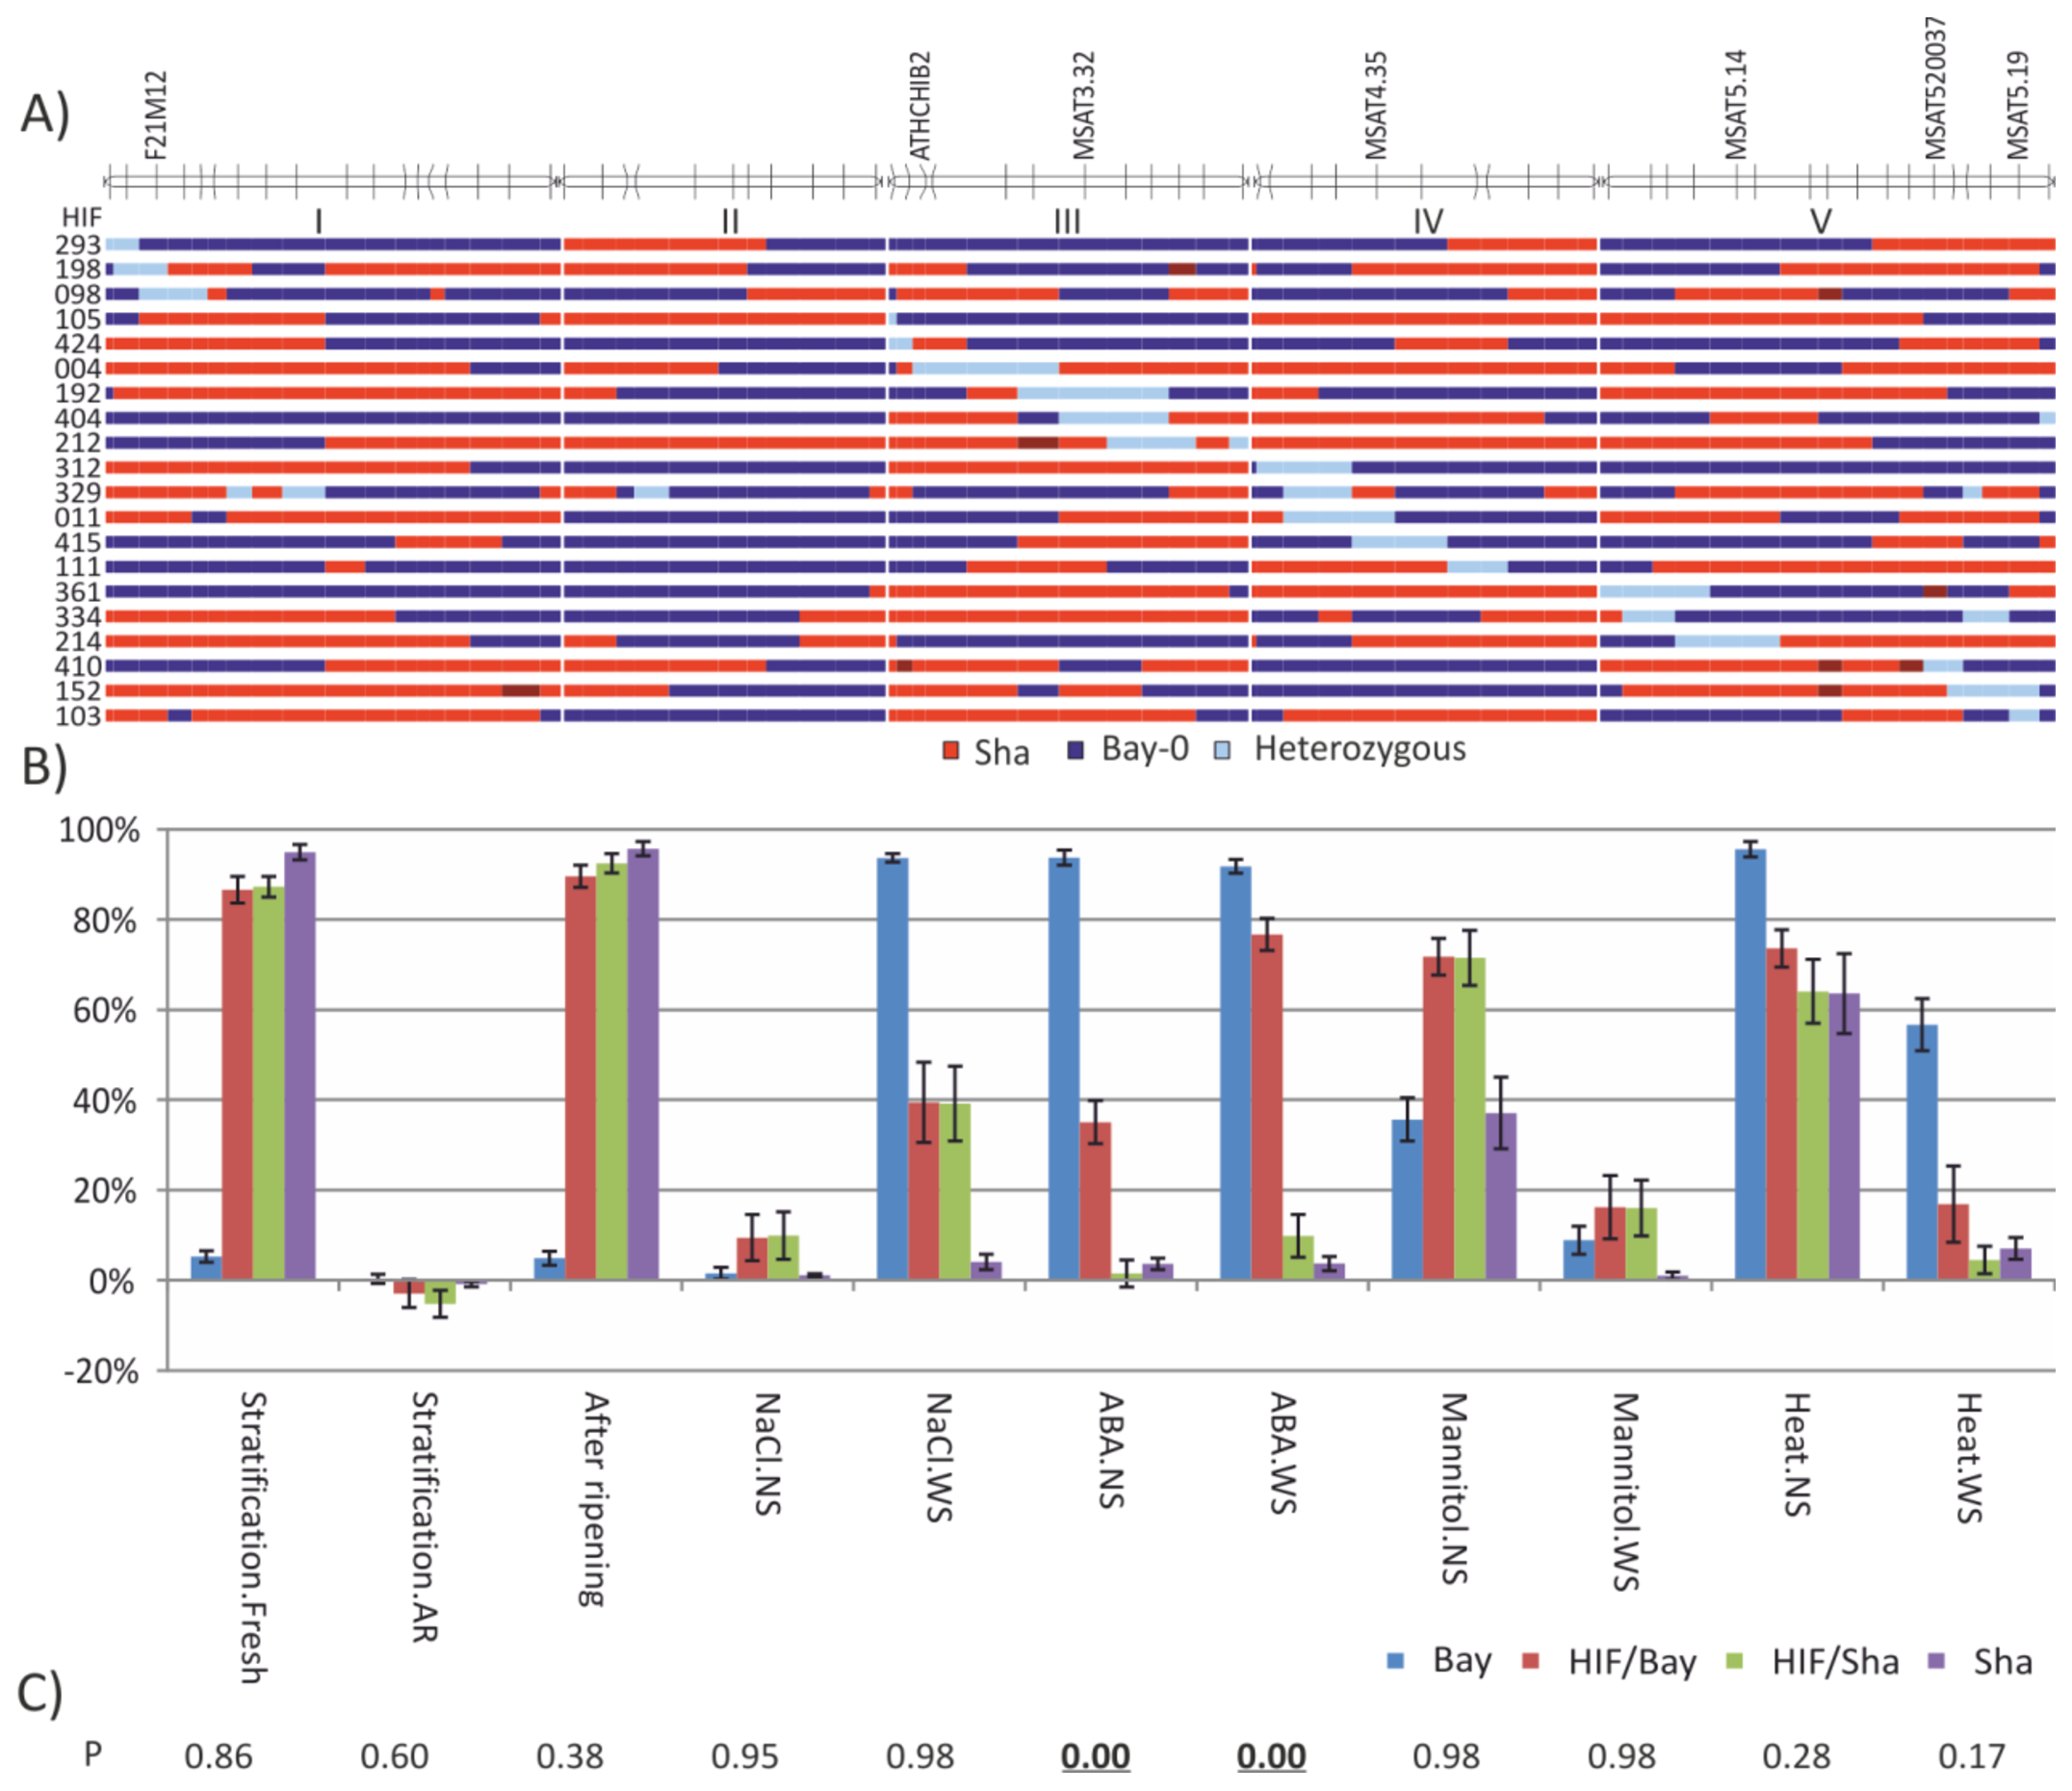
\includegraphics[keepaspectratio,scale=0.30]{eps/image_3_1_8.eps}
  \caption[QTL confirmation.]{Example of the confirmations performed with the HIF approach. A) The blue/red bars 
          indicate the allelic confirmation of the HIF lines used (blue=Bay-0, red=Sha, light blue=segregating). 
          The 5 chromosomes are indicated at the top with the nearest genetic marker for the 7 major loci. B) example 
          analysis for HIF103 (segregating at MSAT5.19, bottom chromosome V). Indicated is the maximum germination 
          (Gmax) for 11 conditions. Error bars represent standard error of at least 6 replicates. Responses are 
          calculated by subtracting the test sample from the control sample as indicated in table \ref{table:codes}. C) T-test 
          significance values for the response values (significant (P<0.05) values are bold).}
          \label{fig:confirmation}
\end{figure}

\begin{figure}[!ht]
  \centering
  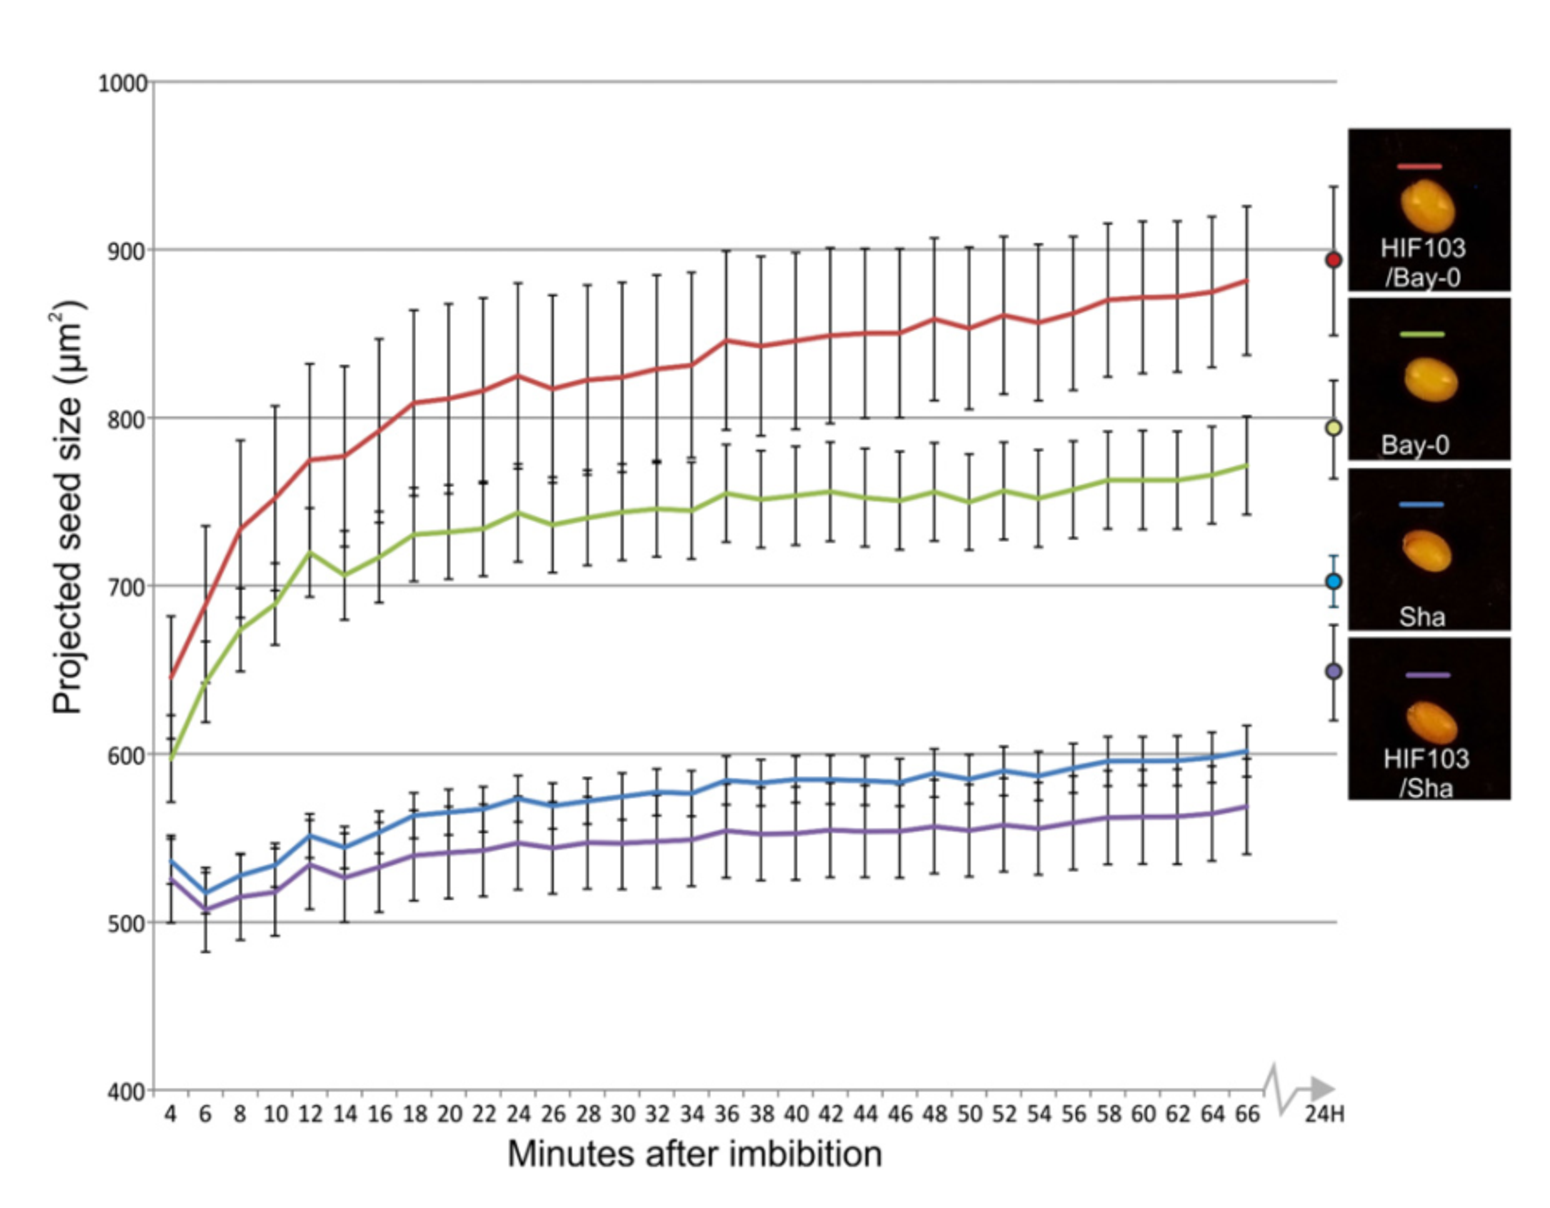
\includegraphics[keepaspectratio,scale=0.30]{eps/image_3_1_9.eps}
  \caption[Seed Swelling.]{Different increases in seed size during the start of imbibition for Bay-0 (green), Sha (blue), 
          HIF103/Bay-0 (red), and HIF103/Sha (purple) seeds. Shown is the average projected seed size area of 10 seeds. 
          Error bars represent SE values. Photographs show 24-h imbibed seeds.}
          \label{fig:swelling}
\end{figure}

\subsection{Conclusions and Discussion}
When analyzing large (RIL) populations, it is hardly feasible to manually count all germination 
experiments several times a day to obtain germination curves. Therefore, previous studies mostly 
restricted to counting end-point germination \cite{Quesada:2002, Alonso-Blanco:2003, Clerkx:2004, 
Laserna:2008, Meng:2008, Bentsink:2010, Galpaz:2010, Vallejo:2010}. A germination curve allows QTL 
mapping under conditions where rate and uniformity are delayed, but maximum germination is not 
affected. Therefore, we used the Germinator package \cite{Joosen:2010} that enabled measurement 
of cumulative germination data and extracting 5 germination parameters that describe the resulting 
germination curve. In the present study we describe several germination QTLs that were not detected 
before in the Bay-0 x Sha population. We observed interesting co-localizations for several germination 
traits and identified the loci that show large effect epistatic interactions. Among these were new 
loci and loci similar to the ones already found in other RIL populations (see \cite{Joosen:2011} - Table 4 for 
the major identified QTL loci).

\subsubsection{Dormancy}
Primary dormancy has been studied extensively in various RIL populations \cite{Bentsink:2010}. These 
authors quantified primary dormancy with the DSDS50 parameter (days of dry storage to reach 50\% 
germination), which is a good measure for after-ripening related dormancy breaking. Although we only 
compared the germination characteristics of freshly harvested seeds with those of after ripened 
seeds and fresh seeds with and without stratification, we detected large genetic variation. Both 
dormancy breaking treatments showed strong QTL at positions 3-2, 4-1 and 5-2, co-locating with DOG6, 
DOG18 and DOG1, respectively (See \cite{Joosen:2011} - Table 4). DOG18 was not detected in a Ler x Sha population and showed a 
stronger dormancy in Ler as compared with An-1, Fei-0 and Kas-2 \cite{Bentsink:2010}. We detected stronger 
dormancy in Sha as compared to Bay-0 at the DOG18 locus. This suggests that both Ler and Sha contain 
an allele of similar strength which is stronger when compared to An-1, Fei-0,  Kas-2 and Bay-0. Remarkably, 
for both the DOG6 and DOG18 location the sensitivity to ABA was higher in Bay-0, whereas dormancy was 
deeper in Sha, which resulted in a directional change of the QTL effect. The more dormant Sha parent 
contains higher initial ABA levels and apparently, after-ripening and 
stratification reduce the ABA sensitivity to a greater extent as compared to the Bay-0 parent. This 
effect was not observed for the DOG1 locus. Further, we identified a strong effect of the dormancy-
breaking treatments on the initiation (t10) and rate (t50) of germination at the bottom of chromosome 5 
(marker MSAT519, 85 cM). The same was observed for germination on mannitol and germination at higher 
temperature. A QTL with opposite effect at this position was found for germination on ABA. Interestingly, 
these co-located with a QTL found for imbibed seed size. 

\subsubsection{Water uptake}
Initiation and rate of germination are highly influenced by the overall water potential of the seed. The 
mucilage layer surrounding the seed appears to play an important role in the process of water uptake 
\cite{Penfield:2001}. Sha is a natural mucilage mutant due to a mutation in the MUM2 gene, which changes 
the hydrophilic potential of rhamnogalacturonan I \cite{Macquet:2007}. Although mucilage has been reported 
to be dispensable for germination and development under lab conditions \cite{Arsovski:2010}, a link with 
germination under reduced water potential conditions was shown by \cite{Penfield:2001}. They showed 
reduced maximum germination of a mucilage-impaired mutant only on osmotic PEG solutions. In our study, 
other traits that co-located on the MUM2 locus were delayed initiation and rate of germination on osmotic
mannitol solution but also on water, which clearly shows the advantage of determining a detailed 
germination curve. We also observed a very strong QTL for swelling of the seed in the first hours of 
imbibition (imbibed seed size) at the MUM2 location. Interestingly, exogenous ABA can be used to 
stimulate mucilage production and ABA-1 mutants are affected in mucilage production \cite{Karssen:1989}. 
This indicates a regulatory role of ABA in mucilage production and fits with our observation of the 
co-localization of a QTL for initiation and rate of germination with a QTL with opposite effect for ABA 
sensitivity. Therefore, we hypothesize that Sha has a slower initiation and rate of germination,
combined with reduced ABA sensitivity due to its mutation in the MUM2 gene. This observation may open 
new research strategies to define the regulatory role of ABA in mucilage production and its multiple 
effects on germination parameters.

\subsubsection{Salt, Heat and ABA}
At the top of chromosome I, underlying marker F12M12, we detected a strong QTL for maximum germination in 
the presence of 100 mM NaCl or 0.5μm ABA. A similar locus has been identified and fine-mapped in a 
Ler x Sha population \cite{Ren:2010}. They identified a premature stop codon in the Response to ABA and 
Salt 1 gene (RAS1; At1g09950) in Sha that led to a truncated protein and showed its role as a negative 
regulator of salt tolerance during seed germination and early seedling growth by enhancing ABA 
sensitivity. Here we show that a similar locus is also inferring tolerance to germination at 30\degree C. 
This suggests an additional role for the RAS1 gene. Increased heat tolerance due to modulation of 
ABA sensitivity has been shown before for other loci, \cite{Argyris:2008,Lee:2010}. 
Interestingly, our present study showed a strong effect of stratification which resulted in a strong 
reduction of significant linkage for NaCl, heat and ABA sensitivity at the F12M12 locus. A specific 
QTL for germination on NaCl preceded by a cold stratification period was found at the middle of 
chromosome I (marker T27K12). Also at this locus we found colocation with sensitivity for germination 
on ABA after stratification. Further fine-mapping at this locus might help to elucidate the effect 
of stratification on ABA mediated abiotic stress tolerance, as well as the apparent overlap of 
dormancy and stress responses. Especially interesting is QTL 5-1 (See \cite{Joosen:2011} - Table 4, and Fig. \ref{fig:gegenomewide}) which mainly 
influences rate and initiation of germination. We detected this QTL for t50 in after ripened seeds 
with stratification treatment, but also for t10 and t50 for germination on salt, regardless of a 
preceding cold stratification and for maximum germination after an accelerated aging treatment. 
One of the genes underlying this QTL interval is a nicotinamidase gene (NIC2, At5g23230), the mutant 
of which has retarded germination and impaired germination potential \cite{Hunt:2007}. These 
authors suggested that NIC2 is normally metabolizing nicotinamide during moist chilling or 
after-ripening, which relieves inhibition of poly(ADP-ribose) polymerase (PARP enzyme) activity and 
allows DNA repair to occur prior to germination. Both accelerated aging and germination under salt 
stress conditions might require optimal functioning of this DNA repair mechanism. Further research 
is needed to determine whether NIC2 is causal for this QTL.

Detection of epistatic interactions in genetic studies can enhance the understanding of underlying 
molecular mechanisms. Recently, \cite{Galpaz:2010} showed strong epistasis in the genetic network 
controlling germination under salt stress in \emph{Arabidopsis}. Due to careful dissection of the epistatic 
relationships they were able to show that three detected QTL rely on the presence of a Columbia 
allele at a QTL on top of chromosome 1. This observation led to the hypothesis that RAS1 
\cite{Ren:2010} functions as a switch of the genetic network by regulating the expression of the 
other QTL. In another study it was found that epistasis significantly influences both fitness and 
germination in \emph{Arabidopsis} \cite{Huang:2010} and novel allele combinations were identified that 
resulted in higher fitness. In our study we detected clear hotspots of epistatic interactions 
between QTL loci on chromosome 3, 4 and 5 (ATHCHIB2, MSAT332, MSAT435, MSAT520037 + MSAT519, 
respectively). This observation strengthens the hypothesis that some of the traits with strong 
QTL co-localizations indeed rely on the same underlying genetic networks.

\subsubsection{Concluding remarks}
We analyzed natural variation for many seed germination characteristics and showed their correlation, 
(shared) QTL positions and epistatic interactions, using a high-throughput phenotyping approach and 
subsequent high-throughput QTL mapping. Using the HIF approach, confirmation of some major QTL 
hotspots was demonstrated, which allows a fast but solid confirmation of a QTL position. Together 
with results from several other studies focusing on genetic variation in seed traits, this study 
has generated an extensive QTL database for Arabidopis and proposed a method of analysis to 
visualize the genetic landscape of seed performance. This database is a solid resource for further 
study. For most of the found loci in this and other studies further characterization, and in most 
cases fine mapping, must be undertaken to elucidate the causal molecular mechanisms. Further, we 
have designed a free available analysis protocol to perform detailed high-throughput QTL analysis 
based on the R/qtl MQM routine. In this era of large-scale phenotyping we regard a detailed analysis 
of QTL, QTLxQTL and QTLxEnvironment interaction as indispensable steps to allow visualization 
and interpretation of multiple traits.



\section{Metabolites in a DesignGG experiment}
A complex phenotype such as seed germination is the resultant of several genetic and environmental 
cues and requires the concerted action of many genes. The use of well-structured recombinant inbred 
lines in combination with omics analysis can help to disentangle the genetic basis of such 
quantitative traits. This so called genetical genomics approach can effectively capture both 
genetic (G) and epistatic interactions (G:G). However, to understand how the environment interacts 
with genomic encoded information (G:E) a better understanding of the perception and processing of 
environmental signals is needed. In a classical genetical genomics setup this requires replication 
of the whole experiment in different environmental conditions. A novel generalized setup overcomes 
this limitation and includes environmental perturbation within a single experimental design. 

We developed a dedicated QTL mapping procedure to implement this approach and used existing 
phenotypical data to demonstrate its power. Additionally, we studied the genetic regulation of 
primary metabolism in dry and imbibed Arabidopsis seeds. Many changes were observed in the 
metabolome which are both under environmental and genetic control and their interactions. 
This concept offers unique reduction of experimental load with minimal compromise of statistical 
power and is of great potential in the field of systems genetics which requires a broad 
understanding of both plasticity and dynamic regulation.

\subsection{Background}
The use of natural variation to disentangle the genetic (G) mechanisms underlying phenotypic differences 
has been very successful both in crop plants and in the model plant Arabidopsis (Arabidopsis thaliana; 
\cite{Alonso-Blanco:2009}. Most of the variation within wild or domesticated plant species is of 
quantitative nature determined by G polymorphisms at multiple loci. Such quantitative trait loci (QTL) 
can beanalyzed efficiently using experimental mapping populations such as recombinant inbred lines (RILs)
derived from directed crosses. Nowadays, many wellstructured RIL populations are available, often 
accompanied with detailed studies of phenotypic variation \cite{Mitchell-Olds:2006}. The complexity 
of quantitative traits is further determined by the interactions between genomic loci (i.e. epistasis) and 
between the genotype and the environment (genetic X environmental [G:E]). While epistasis can be effectively
identified in QTL analyses, albeit with lower power than main effects, the detection of G:E interactions 
requires experimentation in multiple conditions of interest. Because of the large population sizes often 
needed to obtain sufficient statistical power for QTL detection, G:E interactions are usually ignored in 
experimental setups. However, a better understanding of the perception and processing of environmental (E)
signals is greatly needed, because interactions provide important insights in adaptation mechanisms and
evolutionary constraints such as balancing and disruptive selection. To obtain a more detailed view of the
molecular mechanisms underlying phenotypic variation, genetical genomics studies, in which molecular traits
are genetically analyzed, have been successfully applied to enhance a directed strategy to identify causal
relationships \cite{West:2007, Keurentjes:2007, Kliebenstein:2006, Rowe:2008}. The observed phenotype is often the resultant 
of a functional cascade of gene transcription followed by protein translation and modification, which 
finally leads to a highly dynamic metabolome underlying emergent properties \cite{Kooke:2012}. 
With the technological advances made in genomic analytical platforms, such as transcriptomics, proteomics, 
and metabolomics, the large-scale, high-throughput analyses needed for quantitative G approaches have 
become feasible \cite{Jansen:2001a}. 

Incorporating developmental and E  perturbation in the often expensive and laborious omic analyses, an 
alternative experimental setup, coined generalized genetical genomics (GGG), using balanced fractions 
of a RIL population has been proposed \cite{Li:2009}. It provides a cost-effective experimental setup 
for hypothesis-generating research in multiple environments. Such an approach aims for the creation of 
subpopulations of RILs, one for each environment to be tested, with an optimal distribution of parental 
alleles over all available markers \cite{Li:2009}. When these subpopulations are subjected to E 
perturbation, the emerging phenotypes can be explained by several sources of variation: G variation, 
E variation, and G:E variation. Whenever the resulting phenotype is not or only mildly affected by E 
interactions (G:E), the analysis of the different subpopulations can be combined, gaining the full power 
of a complete population. However, when a trait shows strong G:E interaction (e.g. those that only express 
G variation in specific environments), the power to detect QTL is dependent on those subpopulations 
expressing the G variation. Although G:E interactions have been detected previously in genetical 
genomics studies for expression \cite{Li:2006, Smith:2008, Gerrits:2009} and metabolite content 
\cite{Zhu:2012} by analyzing all lines in a population under different environments, the GGG concept 
offers an effective way of studying a combination of G and E perturbations and is of great potential 
in the field of systems genetics, in which a broad understanding of both plasticity and dynamics is 
required \cite{Li:2008}. The fundamental basis of the experimental design and data analysis using a 
full model ($Y = E + G + G:E + e$), where $Y$ is the observed phenotype and $e$ is residual error, 
is generally valid and frequently used \cite{Churchill:2002, Li:2006,Gerrits:2009}. As a proof of 
principle, we present experimental data on the G regulation of primary metabolism in dry and imbibed 
Arabidopsis seeds using a GGG design and discuss the application and implications of such a strategy.

Plants are extremely rich in biochemical compounds, and major roles in plant development, adaptation, 
and defense have been identified for biosynthesis pathways and their products (Binder, 2010). The 
biosynthetic pathways of primary metabolites are well studied and often well conserved between 
different taxa \cite{Peregrin-Alvarez:2009}. Nonetheless, quantitative variation for many of 
these compounds can be observed between natural variants, which might be reflected in their different 
growth characteristics. The analysis of single-gene mutants, for example, has unraveled many key 
components in biochemical pathways and has demonstrated their role in phenotypic traits 
(Fiehn et al., 2000). In Arabidopsis, G variation for many of its metabolic compounds has been 
observed \cite{Kliebenstein:2001, Rowe:2008, Keurentjes:2006}, but G:E interactions 
were ignored in these studies and only addressed by Chan et al.\cite{Chan:2011}. Metabolic profiling at different 
growth stages has further revealed important fluxes that regulate plant development and adaptation 
\cite{Oliveira:2010}. Using the accumulated historical mutations that occur in natural 
variants in combination with metabolic profiling in a generalized design offers the unique possibility 
of identifying G effects over a series of developmental stages. Here, we report on the interaction of 
four different physiological environments (i.e. developmental stages) in dry and imbibed seeds with 
two founder genotypes in a RIL population. To detect the majority of the most prominent primary 
metabolites, we used gas chromatography-mass spectrometry of polar extracts \cite{Roessner:2000, 
Lisec:2008}. These include essential metabolites such as sugars, amino acids, and organic 
acids, which are key compounds in reserve storage and catabolism, growth, and energy metabolism.

The switch from a dry seed, which is equipped for optimal survival and storage of reserves, toward an
imbibed seed, in which energy needed for germination is released and which prepares for autotrophic pro-
duction, is remarkable. Reserves that have been stored during seed maturation are degraded and remobilized
during germination \cite{Bewley:1997,Shu:2008}, a process that is heavily influenced by the capacity 
of carbon/nitrogen partitioning of a maturing seed (Dowdle et al., 2007). Arabidopsis mutants affected 
in their oil reserve content or its mobilization show delayed but not full inhibition of germination 
(Kinnersley and Turano, 2000; Bouché and Fromm, 2004; Shu et al., 2008; Kelly et al., 2011). This suggests 
an additional metabolic switch that occurs during seed desiccation after seed maturation involving a change 
from accumulation of oil and storage proteins to the synthesis of free amino acids, sugars, fatty acids, 
and their degradation products functioning to prepare for rapid metabolic recovery during imbibition 
(Fait et al., 2006; Angelovici et al., 2010). Imbibition of mature seeds specifically shows reduction of 
the metabolites that accumulate during the desiccation period. Upon germination, an increase of many 
metabolites, including amino acids, sugars, and organic acids, can be observed again, which reflects 
the increase of autotrophic activity (Fait et al., 2006). Profiling the primary metabolome over different 
developmental stages in a mapping population is therefore expected to reveal the dynamics of G regulation 
of many of these important processes. We will demonstrate here that much of the observed variation in 
biochemical profiles can be attributed to genotype-by-environment interactions, which can be effectively 
identified in a GGG approach.

\subsection{Results}
In the experimental setup of this study, the E variation is defined as variation observed between the four
developmental stages (PD, AR, 6H, and RP). Significance thresholds, determined by permutation analysis
($n = 1,000, P < 0.01$) for each metabolite, ranged from LOD 3.43 to LOD 3.50 and was stringently set to 
LOD 4 for all analyses. Mapping resulted in 120 significant QTLs in the G component for 83 metabolites and 
31 G:E QTLs for 27 metabolites, ranging from one to four QTLs per metabolite. Thirteen of the G:E QTLs are
significant in the G component as well. For 66 metabolites, no significant QTL was detected. Clustered 
heat maps for both the G and the G:E QTL profiles were created (Supplemental Figs. S4 and S5).

To test the performance of the generalized mapping procedure, QTLs detected in individual environments
using the linear model $Y = G + e$ were compared with QTLs detected in the combined mapping 
approach (using the linear model $Y = E + G + G:E + e$; Fig. 2; Supplemental Table S1).
QTLs were binned in upper or lower chromosome arms to reduce the effects of small positional shifts.
Results were plotted in a network, with nodes representing QTLs connected with edges to nodes repre-
senting the mapping populations in which they were detected (Fig. 2). QTLs are grouped in three sections
according to their detection in the different mapping procedures. The middle section shows 73 QTLs that
were detected in both the $Y = E + G + G:E + e$ model and in one or more single-environment mappings 
using the $Y = G + e$ model. This shows that most of the G variation present in the single environments 
can effectively be captured by using the generalized model.

The presence of 60 QTLs that were only significantly detected in the $Y =E + G + G:E + e$ model 
(right section) shows the combined power of the generalized approach and the usage of more genotypes. 
These QTLs are not detected in the single-environment mapping in which only 41 individuals were used.
Combining all data across all environments in the linear model increases power to detect QTLs, but it
should be noted that there are also 20 minor QTLs (leftsection) that are only significant in the single
environment mapping using the $Y = G + e$ model. These QTLs are not detected in the $ Y = E + G + G:E + e$
model. This can be explained by two factors: (1) environments in which the G variation is not expressed
introduce noise in the experimental data and thereby decrease mapping power, and (2) deviations from a
balanced allele distribution in the different subpopulations can introduce some stochasticity around the
threshold level, although this is not the case in our data.

Importantly, all major-to-moderate-effect-size QTLs could be detected using the generalized model, even
when these QTLs were not detected in the separate environment models. Although it is difficult to 
compare power with the latter models, because population sizes differ, the generalized design 
efficiently identifies all relevant QTLs, which were detected by the four separate models, and in addition, 
it detects G:E interactions. In a general exploratory study, the reduction in experimental burden therefore 
amply outweighs the incidental failure to detect the limited number of small-effect QTLs. The application 
of a GGG design can thus be an important advancement in evolutionary and ecological studies assessing 
the contribution of G and E effects to natural variation in life history traits.

For breeding purposes, the allelic effect size is an important measure, and differentiation of the 
environment in which the allelic effect is expressed can be very useful. In the generalized setup, 
the allelic effect size of those metabolites with significant QTLs is separated per environment 
(Supplemental Files S4 and S5). For every QTL that is consistently detected in all four conditions, 
a LOD score for G effect (Fig. 3,x axis) is obtained from full-model mapping. For these QTLs,
normalized allelic effect sizes are calculated by Zscore transformations for each environment 
(Fig. 3, y axis). QTLs detected in the G component of the linear model (Fig. 3A) show an expected 
linear relationship between LOD score and effect size in all measured environments. This correlation 
is much weaker for QTLs detected in the G:E component of the linear model (Fig. 3B) because the G 
variation is not expressed in all environments. QTLs of metabolites with strong G:E interaction, 
therefore, display larger effect sizes in fewer environments compared with G-component QTLs of 
similar significancelevels.

Clearly, the choice of environments used in these studies is crucial (Li et al., 2008). Limited power 
can be expected when environments vary too much and no overlapping G variation is present, and 
contrarily, there is hardly any additive value of the design when using very similar environments. 
In this study, we carefully selected four biologically relevant developmental stages of seed germination 
with expected variation in metabolite levels to different extent and consider them as an E factor in 
the follow-up statistical analysis. The selected developmental stages start from PD dry seeds to 
seeds at the point of RP. The first two stages, being freshly harvested PD and AR nondormant dry 
seeds, respectively, are expected to comprise a very similar metabolome, as most, if not all, metabolic
fluxes are arrested in the dry seed. The other two stages represent 6H seeds and seeds at RP, respectively.
Different levels of E variation were obtained and could be mapped by the G and/or G:E component of 
the linear model.

\subsubsection{Confirmation of Metabolic QTLs}
To independently confirm the effect of a single locus, it must be isolated and tested in an isogenic 
background. Several methods can be followed to perform such an independent confirmation of QTLs. A 
powerful approach is the use of residual heterozygosity in early generations of RILs. The Bay-0XSha 
RIL population(420 lines in total) was genotyped at F6, in which approximately 97\% homozygosity is 
reached in each line. This resulted in the presence of residual heterozygosity in at least a single 
RIL at almost all genome positions. Those heterozygous regions are segregating in a Mendelian fashion 
in the next generation and can be used to confirm QTL positions, as it provides a possibility to
study both parental alleles at the locus of interest in an otherwise homozygous background 
(Tuinstra et al., 1997). In a heterogeneous inbred family (HIF), those heterozygous regions are fixed, 
and two separate lines containing the alleles of both parents, respectively, are maintained.

HIF312 and HIF214 are segregating for regions at the top of chromosomes 4 and 5 (Fig. 6A), respectively,
and cover the region in which the two major metabolite hotspots were detected. AR dry seeds were used to
profile the HIFs for metabolic content because many of the QTLs detected in this region showed a 
large-effect size at the dry seed stages. Significant differences between parental alleles using four 
replicates were defined by a two-tailed Student's t test($P < 0.05$). In total, 34 out of 64 QTLs could 
be confirmed using this approach (Supplemental Fig. S8). For maltose, for instance, two QTLs with 
opposite direction were found (Fig. 6B), which could both be confirmed using the two distinct HIFs 
(Fig. 6C). In a number of cases, a HIF effect was observed that was not detected significantly
in the RIL population (e.g. digalactosylglycerol). This might be the result from the higher power in 
near isogenic lines due to the absence of epistatic interactions (Keurentjes et al., 2007b). Nonetheless, 
a substantial number of QTLs could not be confirmed by the HIF lines. The enrichment for small-effect 
QTLs in the unconfirmed class suggests that four replicates generate insufficient power to identify 
significant differences for these metabolites in the HIF experiments, although we cannot rule out that 
they are false positives from the QTL analysis. Furthermore, QTLs depending on epistatic interactions 
cannot be detected in some near-isogenic lines. In addition, a number of QTL support intervals are 
broader than the region covered by the HIF, and thus, the causal G polymorphism within the QTL interval, 
but outside the region covered by the HIF, would have been missed.

The analyses of the HIF lines indicate that most of the large-effect QTLs can be accurately detected 
using a generalized genomics approach. Although an underestimation of small-effect QTLs can be expected, 
this is largely compensated by the higher power of detecting G and E interactions



\chapter{High throughput data analysis}
\label{chap:xqtlwormbench}

\emph{The major challenge in bioinformatics comes from the huge amount of data collected and the 
multitude of technologies used. We developed the xQTL workbench system\cite{Arends:2012} to store 
large amounts of phenotype and genotype data in the XGAP \cite{Swertz:2010a} dataformat. xQTL 
workbench can easily be adapted to a multitude of input and storage formats using the MOLGENIS 
\cite{Swertz:2004} generator. xQTL workbench uses the power of distibuted computing to allow 
massive parrallel QTL analysis and allows new analysis tools to be quickly added to the system, 
an application of the xQTL system is found in the WormQTL database \cite{Snoek:2012}.}

\null
\vfill

\begin{myexampleblock}{Originally published as:}
  \authors{Morris A Swertz, Martijn Dijkstra, ..., Danny Arends, George Byelas, et al}\\
  \emph{The MOLGENIS toolkit: rapid prototyping of biosoftware at the push of a button}\\
  \bold{BMC Bioinformatics} (2010)\\\\

  \authors{Morris A Swertz, K Joeri van der Velde, Bruno M Tesson, ..., Danny Arends, et al}\\
  \emph{XGAP: a uniform and extensible data model and software platform for genotype and phenotype experiments}\\
  \bold{Genome Biology} (2010)\\\\

  \authors{Danny Arends*, K. Joeri van der Velde*, Pjotr Prins, Karl W. Broman, Steffen Moller, et al.}\\
  \emph{xQTL workbench: a scalable web environment for multi-level QTL analysis}\\
  \bold{Bioinformatics} (2012)\\\\

  \authors{L. Basten Snoek*, Joeri Van der Velde*, Danny Arends*, Yang Li*, Antje Beyer, et al.}\\
  \emph{WormQTL: Public archive and analysis web portal for natural variation data in Caenorhabditis spp}\\
  \bold{Nucleic Acids Research} (2012)
\end{myexampleblock}

\newpage

\section{Reusable software (MOLGENIS)}
\subsection{Background}
High throughput technologies have boosted biological and medical research and the need for software 
infrastructures to manage and process the large datasets produced is widely accepted \cite{Swertz:2007,
Stein:2008, Thorisson:2009}. Bioinformaticians are under continuous pressure to both tackle the complexity 
and diversity of new biological systems and analytical methods and to translate these quickly into 
flexible informatics infrastructures, while keeping up with the unpredictable evolution of molecular 
biotechnologies and the increasing scale of experiments. While standardization of tools and data formats 
in open source projects like the Generic Model Organism Database, GMOD \cite{OConnor:2008}, and the 
Open Bioinformatics Foundation, OBF \cite{OBF:2010:Online}, have been indispensable in reducing the 
development efforts needed via reusable and easy to integrate components, new research must also be 
quickly accommodated, for which efficient software variation mechanisms are needed.

We present the evolution of MOLGENIS into a generic, model-driven toolkit for the rapid generation of 
data-intensive biosoftware applications \cite{Swertz:2010a}. Figure \ref{fig:modelDrivenDevelopment} 
outlines the 'model-driven' development method that several bioinformatics projects adopted in recent 
years to enable fast and flexible infrastructure development. We demonstrate step-by-
step how bioinformaticians can use a domain-specific language to efficiently model the biological 
details of their particular biological system, and use MOLGENIS software generation tools to 
automatically generate a web application tailored to the experiments of their biologists, 
building on reusable components. Next, we evaluate the results of these methods in the development 
of a range of MOLGENIS applications \cite{Swertz:2004, Swertz:2010a, Thorisson:2009, Leu:2010, 
Li:2009, Smedley:2008}, that is, software applications generated using the MOLGENIS toolkit. We found 
up to 30 times efficiency improvement compared to hand-writing software, while providing a richness 
of features practically unfeasible to produce by hand but not yet provided by related projects. We 
conclude by inviting the bioinformatics community to add more MOLGENIS models, components and 
generators to quickly generate all the software infrastructures biologists want to have.

\begin{figure}[h!]
  \centering
  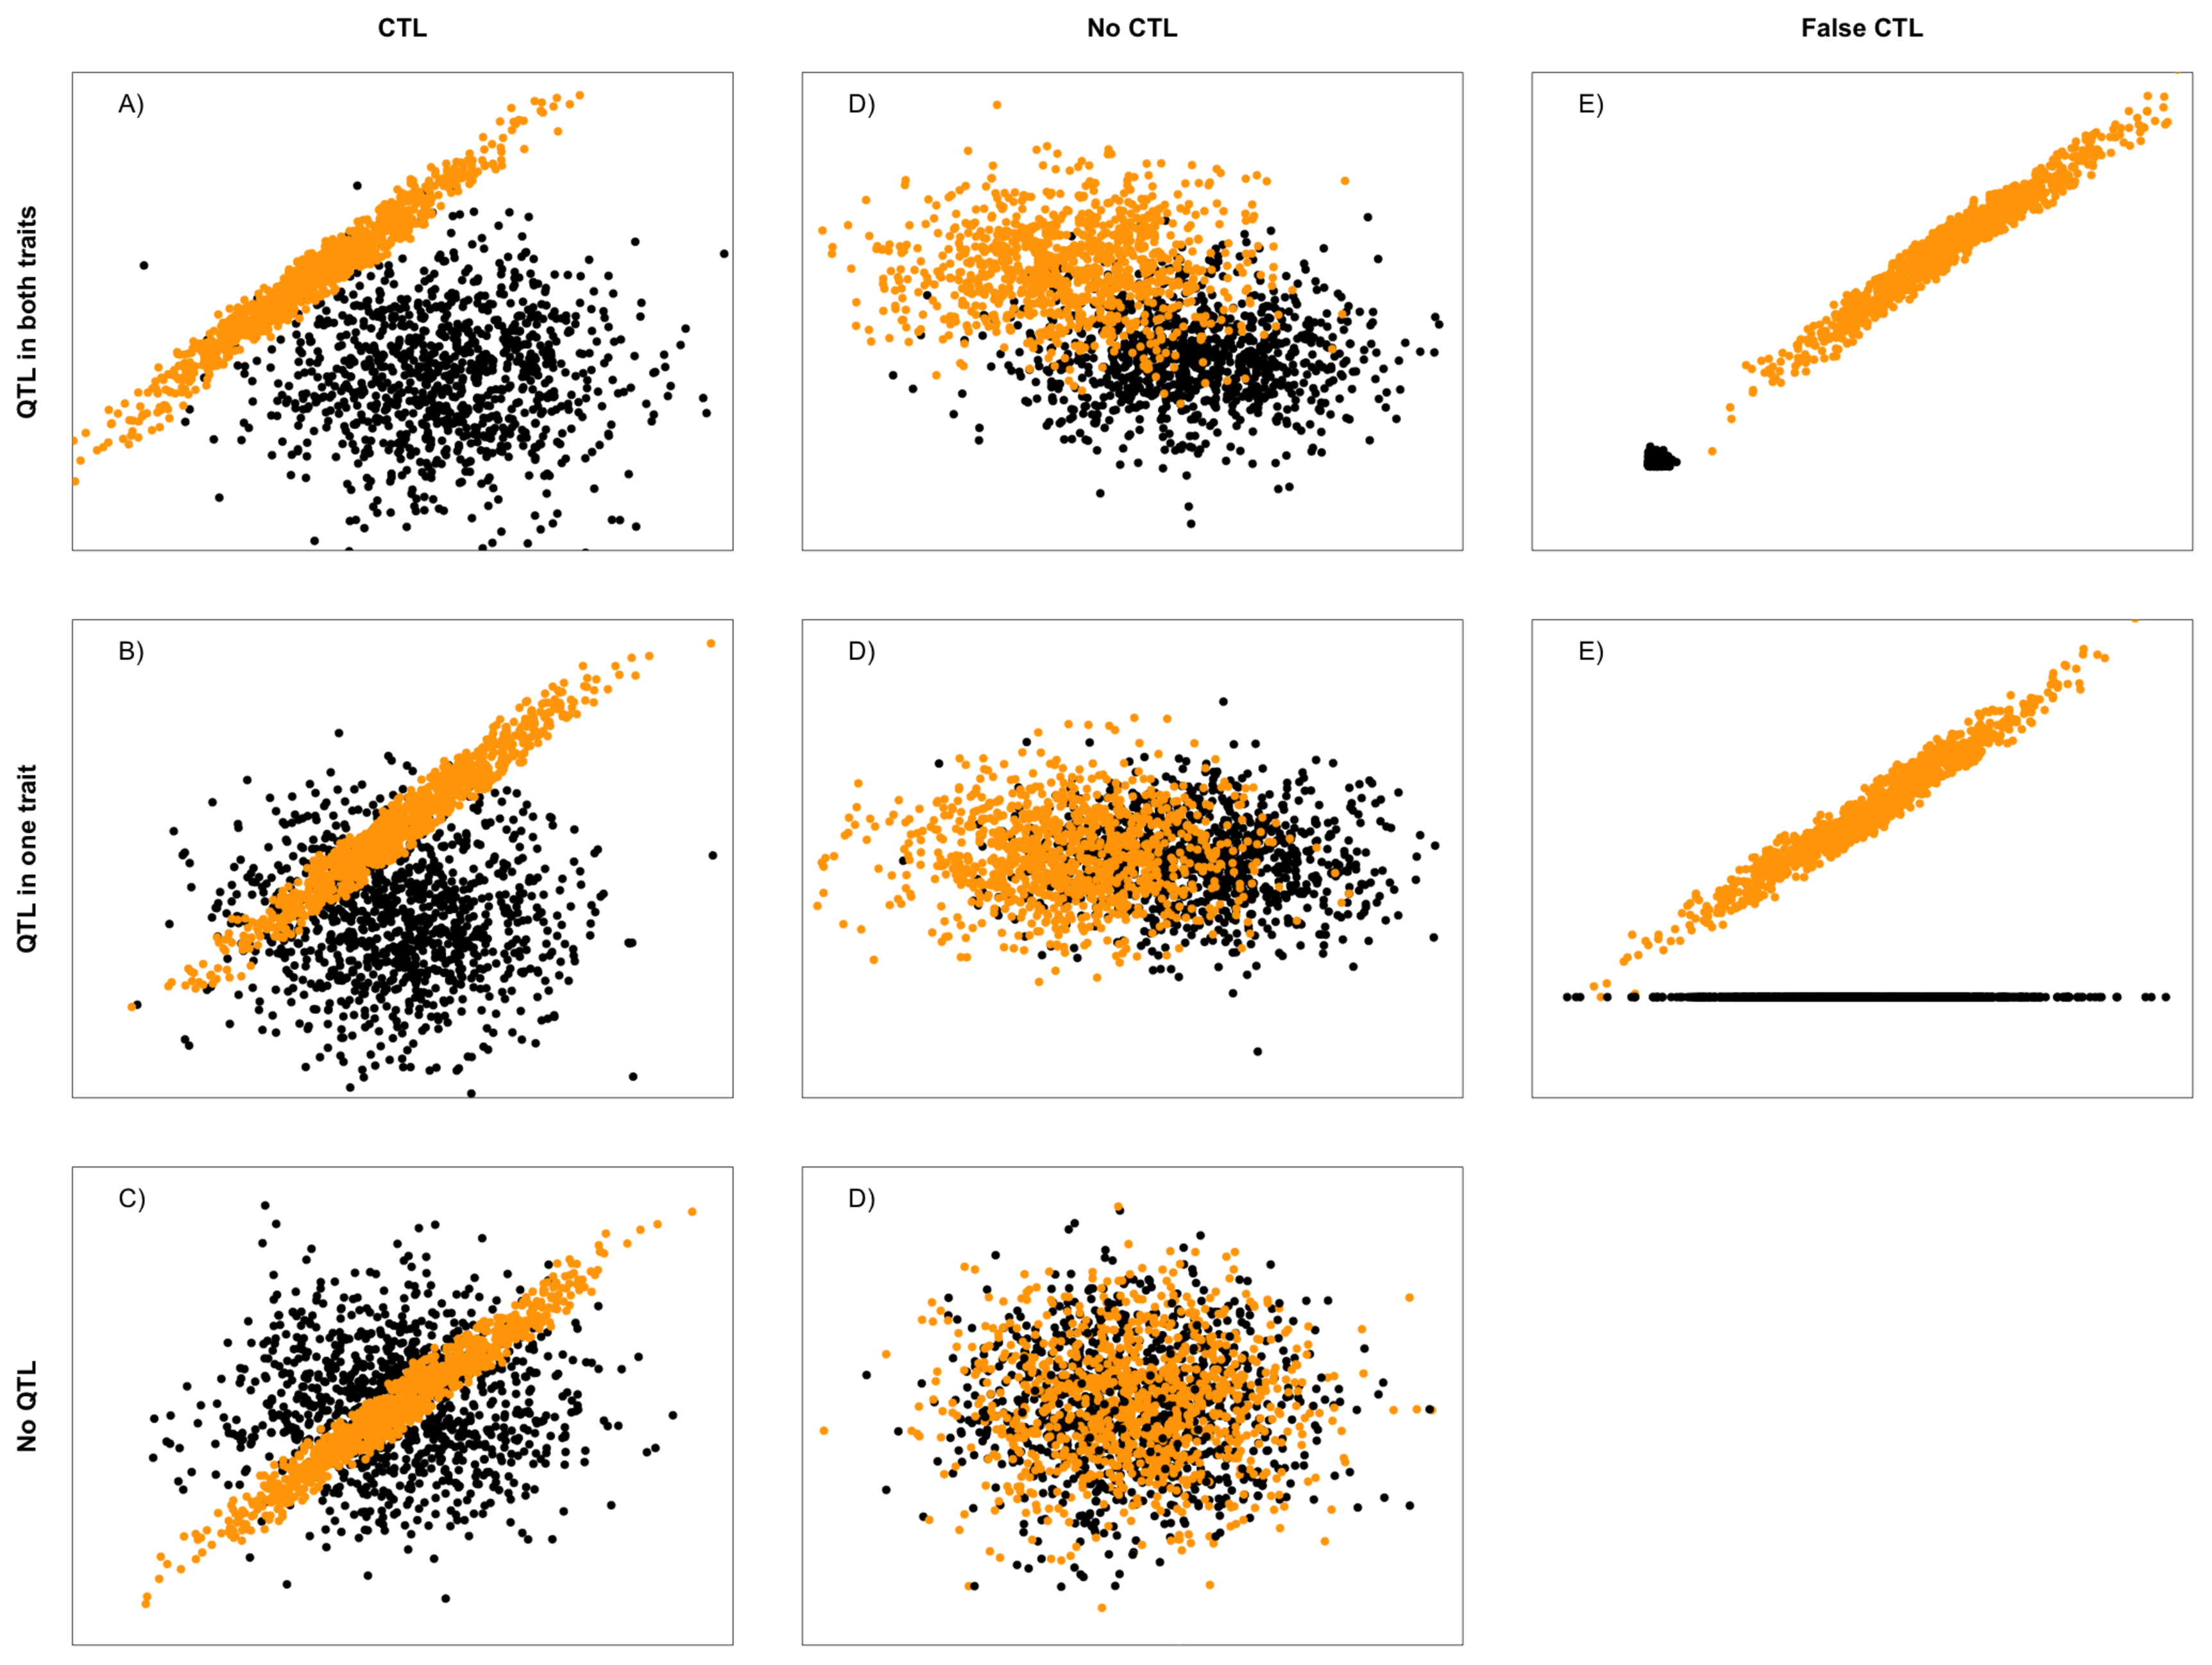
\includegraphics[width=1.0\textwidth]{eps/image_4_1.eps}
  \caption[MOLGENIS]
    {Many minor and major changes have to be written in software code before a 'standard' software infrastructure 
    accommodates a particular research. Using 'model-driven' development methods a bioinformatician only need to 
    model what is needed for his experiment using a therefore optimized domain specific language (DSL). Generators 
    quickly produce all the software logic to compose a full software infrastructure that accommodates these needs. 
    When experimental needs change, a bioinformatician can (re)run the same generator with an adapted model file 
    to quickly produce another variant of software infrastructure. This vastly reduces 'time-to-research' and 
    enables bioinformaticians to quickly develop a suite of software infrastructures, with each variant accommodating 
    a specific research task, while still on track to reuse, integrate and share the best standard features with 
    other labs and bioinformaticians.}
    \label{fig:modelDrivenDevelopment}
\end{figure}

The MOLGENIS toolkit is based on the method of model-driven development which emerged in the 1990s 
from the computer industry. Below we discuss the MOLGENIS' modeling language, the generators and 
reusable components. 

\subsubsection{Modeling language}
A custom MOLGENIS application can be defined in a single file. The file is written in MOLGENIS' 
modeling language. One can think of MOLGENIS' modeling language as a 'domain-specific language' 
\cite{Deursen:2002}, in this case to compose biosoftware infrastructures.

In most cases, knowledge of the DSL is all that is needed to produce a custom MOLGENIS application 
variant. The domain-specific language was implemented using XML so that model files can be edited 
using off-the-shelf XML editors. However, you may want to include hand-programmed components into 
a particular MOLGENIS instance. For example, for the eXtensible Genotype And Phenotype (XGAP) 
database application of MOLGENIS \cite{Swertz:2010a}, we developed a 'MatrixViewer' that builds on the generated 
components, which saved us the work of writing the plug-in from scratch. This requires a model 
sentence that points to the 'plug-in' (allowing it to be seamlessly integrated) as well as 
hand-programming of the plug-in itself.

\subsubsection{Reusable components}
Each MOLGENIS application follows the widely accepted three-layered architecture design of web 
applications. MOLGENIS' reusable components provide building blocks with a modular structure, which 
allows them to be assembled in diverse combinations, similar to prefabricated houses that are built 
from modular walls instead of bricks. Some building blocks are semi-finished and need to be 
'completed' before use (which is automated in MOLGENIS via the generators and inheritance). We based 
the design of MOLGENIS on industry-proven design patterns from the 'patterns for enterprise 
application architecture' (PEAA), a catalog of proven solutions for software design problems 
that we used as a guideline \cite{Fowler:2002}. The logic of the reusable components is implemented using 
Java (http://java.sun.com); the HTML layout for the user interface is encoded in Freemarker 
templates (http://freemarker.sourceforge.net/); and the database back-end using MySQL, PostgreSQL 
or HSQLDB.

\begin{figure}[h!]
  \centering
  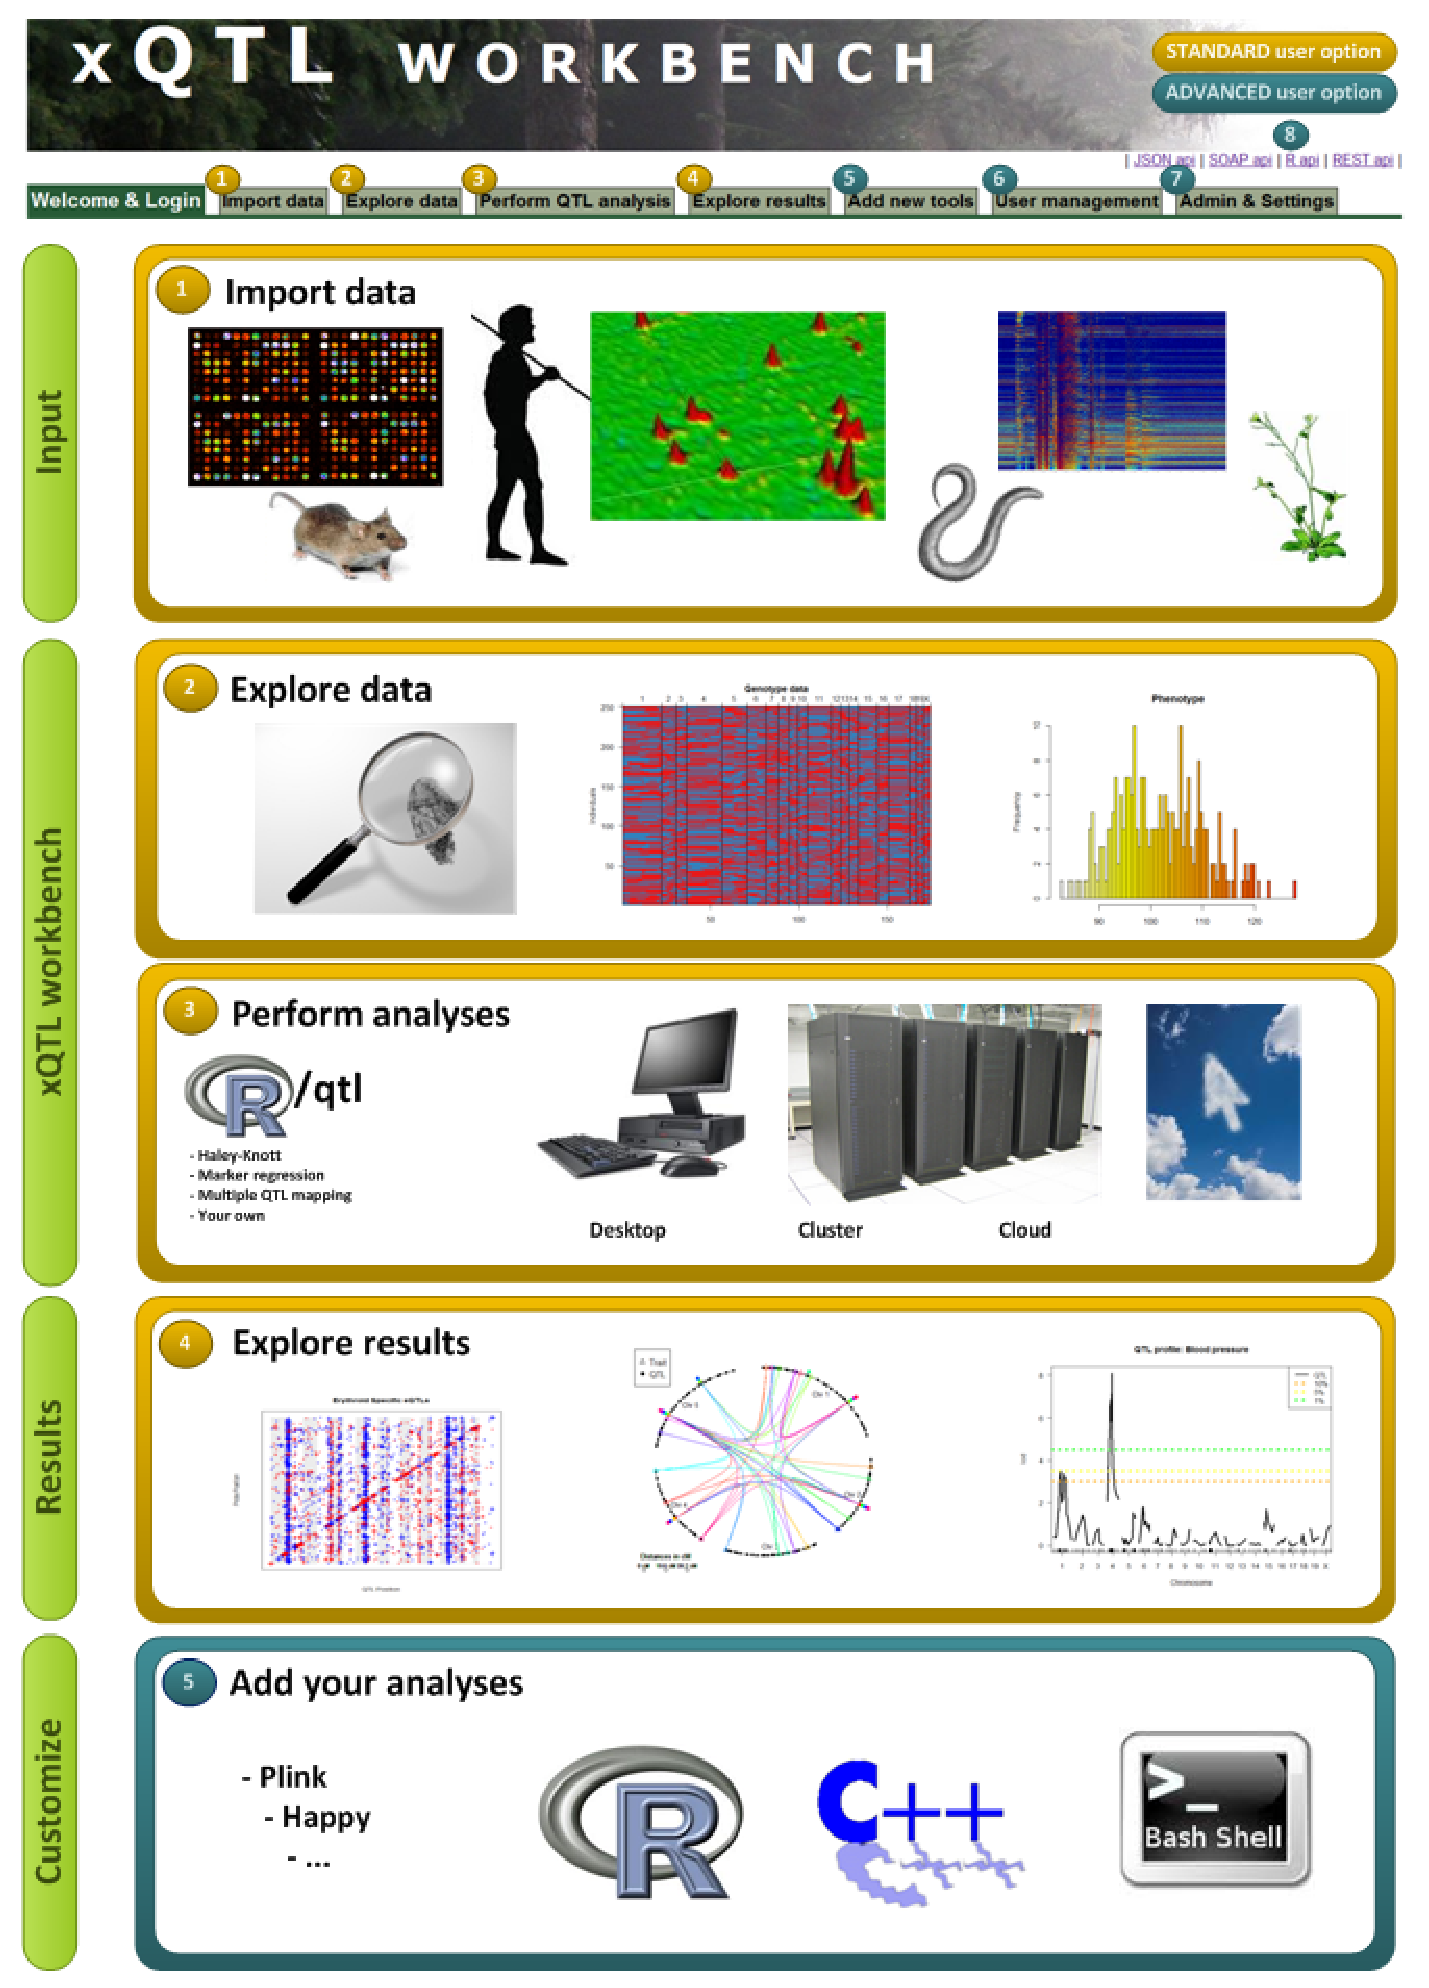
\includegraphics[width=1.0\textwidth]{eps/image_4_2.eps}
  \caption[Templates]
    {MOLGENIS generators are implemented as templates. This example shows the generator for a database component 
    (A). This template is applied to each <entity> in the model to generate many complete DataMappers that would 
    otherwise need to be written by hand. (B) shows an example of the generated source files, in this case for 
    <entity name="Experiment"> as described in Figure 1. The command \$Name(entity) translates to the name of the 
    entity ("Experiment") and command \${csv(\$entity.Fields, x)} means that command 'x' is applied to each field 
    of the entity and returned as a comma separated string (csv).}
	\label{fig:Generators}
\end{figure}

\subsubsection{Generators}
The generators are compact specifications of how each database feature should be implemented. 
The MOLGENIS toolkit now has over 20 generators, but normal users will never need to take a look 
inside. However, for readers wanting to create their own generators, figure \ref{fig:Generators} provides an example 
of the simple, text-based, generators we use. Each generator consists of two files: a Freemarker 
template that describes the code to be generated (similar to that shown in figure \ref{fig:Generators}a) and a Java 
'Generator' class that controls the generating process. A new generator can be developed as 
follows: First write some examples of the desired programs by hand, where possible using similar 
patterns and mark which parts are variable between them. Then copy one of these examples into 
a generator template (text file) and replace all variable parts with 'holes' that 
are to be filled by the code generator based on parameters from DSL. At each generation, the 
template is then automatically copied and the 'holes' filled, based on parameters described in 
the domain-specific language, saving much laborious manual work. 

\subsection{Results}
To start generating your own MOLGENIS application, you can download a ready-to-use 'workspace' 
from http://www.molgenis.org, which can be edited using the commonly used Eclipse integrated 
development environment (IDE) tool (http://www.eclipse.org). Extensive manuals are available to 
help install the Java, MySQL, Tomcat and Eclipse software needed and to learn how to walk through 
the Eclipse workspace to edit models and generate and run MOLGENIS instances; most new users can 
complete this part in about three hours. Below we summarize the output you can expect as well 
as recent experiences from using this toolbox. Detailed examples on how these features can be 
used to support actual microarray or genetical genomics experiments can be found in \cite{Swertz:2010a, Li:2009, Smedley:2008}.

After completing a MOLGENIS model and running the generator as described above, you have a 
ready-to-use software application. The features you get when running the generated result as 
a web application: a fully functional system where researchers can upload, manage, browse 
and query their biological data that conform to the model, optionally enhanced with analysis 
tools to explore and annotate (depending on the plug-ins).

\subsubsection{Applications}
Since the earliest MOLGENIS application \cite{Swertz:2004}, we have successfully evaluated use of the MOLGENIS 
toolkit to build a wide range of biomedical applications \cite{Swertz:2010a, Fredman:2002, Leu:2010, Li:2009, Smedley:2008}, 
ranging from sequencing to proteomics, including:

\begin{enumerate}\itemsep1pt
\item \emph{XGAP} - an eXtensible Genotype And Phenotype platform \cite{Swertz:2010a} for systems genetics 
(GWAS, GWL) to store all kinds of *omics data ranging from genotype to transcript and protein 
data. XGAP comes with plug-ins to view large data matrices and run processing tools on a cluster. 
See http://www.xgap.org
\item \emph{Pheno-OM} - to integrate any phenotype data from locus-specific annotations to 
rich biobank cohort reports with the help of the OntoCAT ontology toolkit to create semantic 
mappings between related data items \cite{Kurbatova:2011}.\\
See: http://www.ebi.ac.uk/microarray-srv/pheno
\item \emph{FINDIS} - a mutation database for monogenic diseases belonging to the Finnish 
disease heritage. See http://www.findis.org/
\item \emph{HGVBaseG2P} - the data management and curation interface complement for HGVbaseG2P, 
a central database of genotype to phenotype association studies \cite{Fredman:2002}. See http://www.hgvbaseg2p.org
\item \emph{MAGETAB-OM} - a microarray experiment data platform based on the MAGE-TAB data format 
standard to create a local microarray repository that is compatible with the public ArrayExpress 
and GEO repositories. See http://magetab-om.sourceforge.net/ 
\item \emph{NordicDB} - the database of high-density genome-wide SNP information from 5,000 
controls originating from Finnish, Swedish and Danish studies \cite{Leu:2010}. See http://www.nordicdb.org
\item \emph{DesignGG} - a web tool to optimally design such genetical genomics experiments \cite{Li:2009}. 
See http://gbic.biol.rug.nl/designGG/
\end{enumerate}

A full list MOLGENIS applications can be found at http://www.molgenis.org. Each of these MOLGENIS projects 
reported major benefits from the short cycle from model to running system to enable quick evaluation 
(500 lines of model XML replaces 15,000 lines of programming code) and use of the batch loading of 
data to evaluate how the newly built system works with real data. More often than not, MOLGENIS 
helped in finding inconsistencies in existing data that would otherwise have gone unnoticed, leading 
to experimental errors. In our experience, a typical MOLGENIS generator run gives you about 90\% of 
the application that is desired 'for free', with the remaining 10\% typically filled in using plug-ins 
that are written by hand. The MOLGENIS toolkit has also been used to extend or replace existing 
software applications: the ExtractModel tool allows you to generate a MOLGENIS application from an 
existing database, which can then be run side-by-side with code developed previously, providing the 
best of both generated and hand-written worlds.

\subsection{Conclusions and Discussions}
In a recent perspective paper \cite{Swertz:2007} we evaluated the general benefits and pitfalls of model-driven 
development, such as the ability to develop infrastructure in short cycles to get the application 
right, ensuring developers and biologists are thinking along the same lines and increasing quality 
and functionality for all. We further evaluated applying this method to both microarray and genetical 
genomics experiments \cite{Swertz:2004}, \cite{Swertz:2010a}.

Here we have presented MOLGENIS in detail and reported the results of using this method against a 
wider range of applications. We conclude that using model-driven methods enables bioinformaticians 
to build biological software infrastructures faster than before, with the additional benefit of 
much easier sharing of models, data and components. Much less time is spent on customizing and gluing 
together individual components. The result is of higher quality because fewer incidental errors creep 
into the applications as a consequence of the automated procedures; best practices are applied 
instead of reinvented. And you do not need heavy-weight technology to implement a model-driven 
generator: simple text-based templates suffice to create biological software generators.

As a next step we want to expand the MOLGENIS toolkit to also generate data processing tools, 
including user friendly interaction, building on other 'model-driven bioinformatics' projects 
in this area, such as Taverna \cite{Oinn:2004} to model/execute analysis workflows and Galaxy 
\cite{Goecks:2010} to generate user interfaces for processing tools. We hope that many 
bioinformaticians will enforce our open source efforts and share their best models, 
plug-ins and generators at http://www.molgenis.org, so that, in time, every biologist may 
find a MOLGENIS variant that suits his/her needs.

\section{Storing extensible data (XGAP)}
We present an extensible software model for the genotype and phenotype community, XGAP. Readers 
can download a standard XGAP (http://www.xgap.org) or auto-generate a custom version using 
MOLGENIS with programming interfaces to R-software and web-services or user interfaces for 
biologists. XGAP has simple load formats for any type of genotype, epigenotype, transcript, 
protein, metabolite or other phenotype data. Current functionality includes tools ranging 
from eQTL analysis in mouse to genome-wide association studies in humans.

\subsection{XGAP - A minimal and extensible object model}
We developed the XGAP objectmodel to uniformly capture the wide variety of (future) genotype 
and phenotype data, building on generic standard model FuGE (Functional Genomics Experiment) 
\cite{Jones:2007} for describing the experimental 'metadata' on samples, protocols and experimental variables 
of functional genomics experiments, the OBO model (of the Open Biological and Biomedical 
Ontologies foundry for use of standard and controlled vocabularies and ontologies that ease 
integration \cite{Smith:2007}, and lessons learned from previous, profiling 
technology-specific modeling efforts \cite{Brazma:2006}.

Figure \ref{fig:XGAP}b shows the core components of a genotype-to-phenotype investigation: the biological 
subjects studied (for example, human individuals, mouse strains, plant tissue samples), the 
biomolecular protocols used (for example, Affymetrix, Illumina, Qiagen, liquid 
chromatography/mass spectrometry (LC/MS), Orbitrap, NMR), the trait data generated (usually 
data matrices with, for example, phenotype or transcript abundance data), the additional 
information on these traits (for example, genome location of a transcript, masses of LC/MS peaks), 
the wet-lab or computational protocols used (for example, MetaNetwork \cite{Fu:2007} in the case of QTL and
network analysis) and the derived data (for example, QTL likelihood curves).

\begin{figure}[h!]
  \centering
  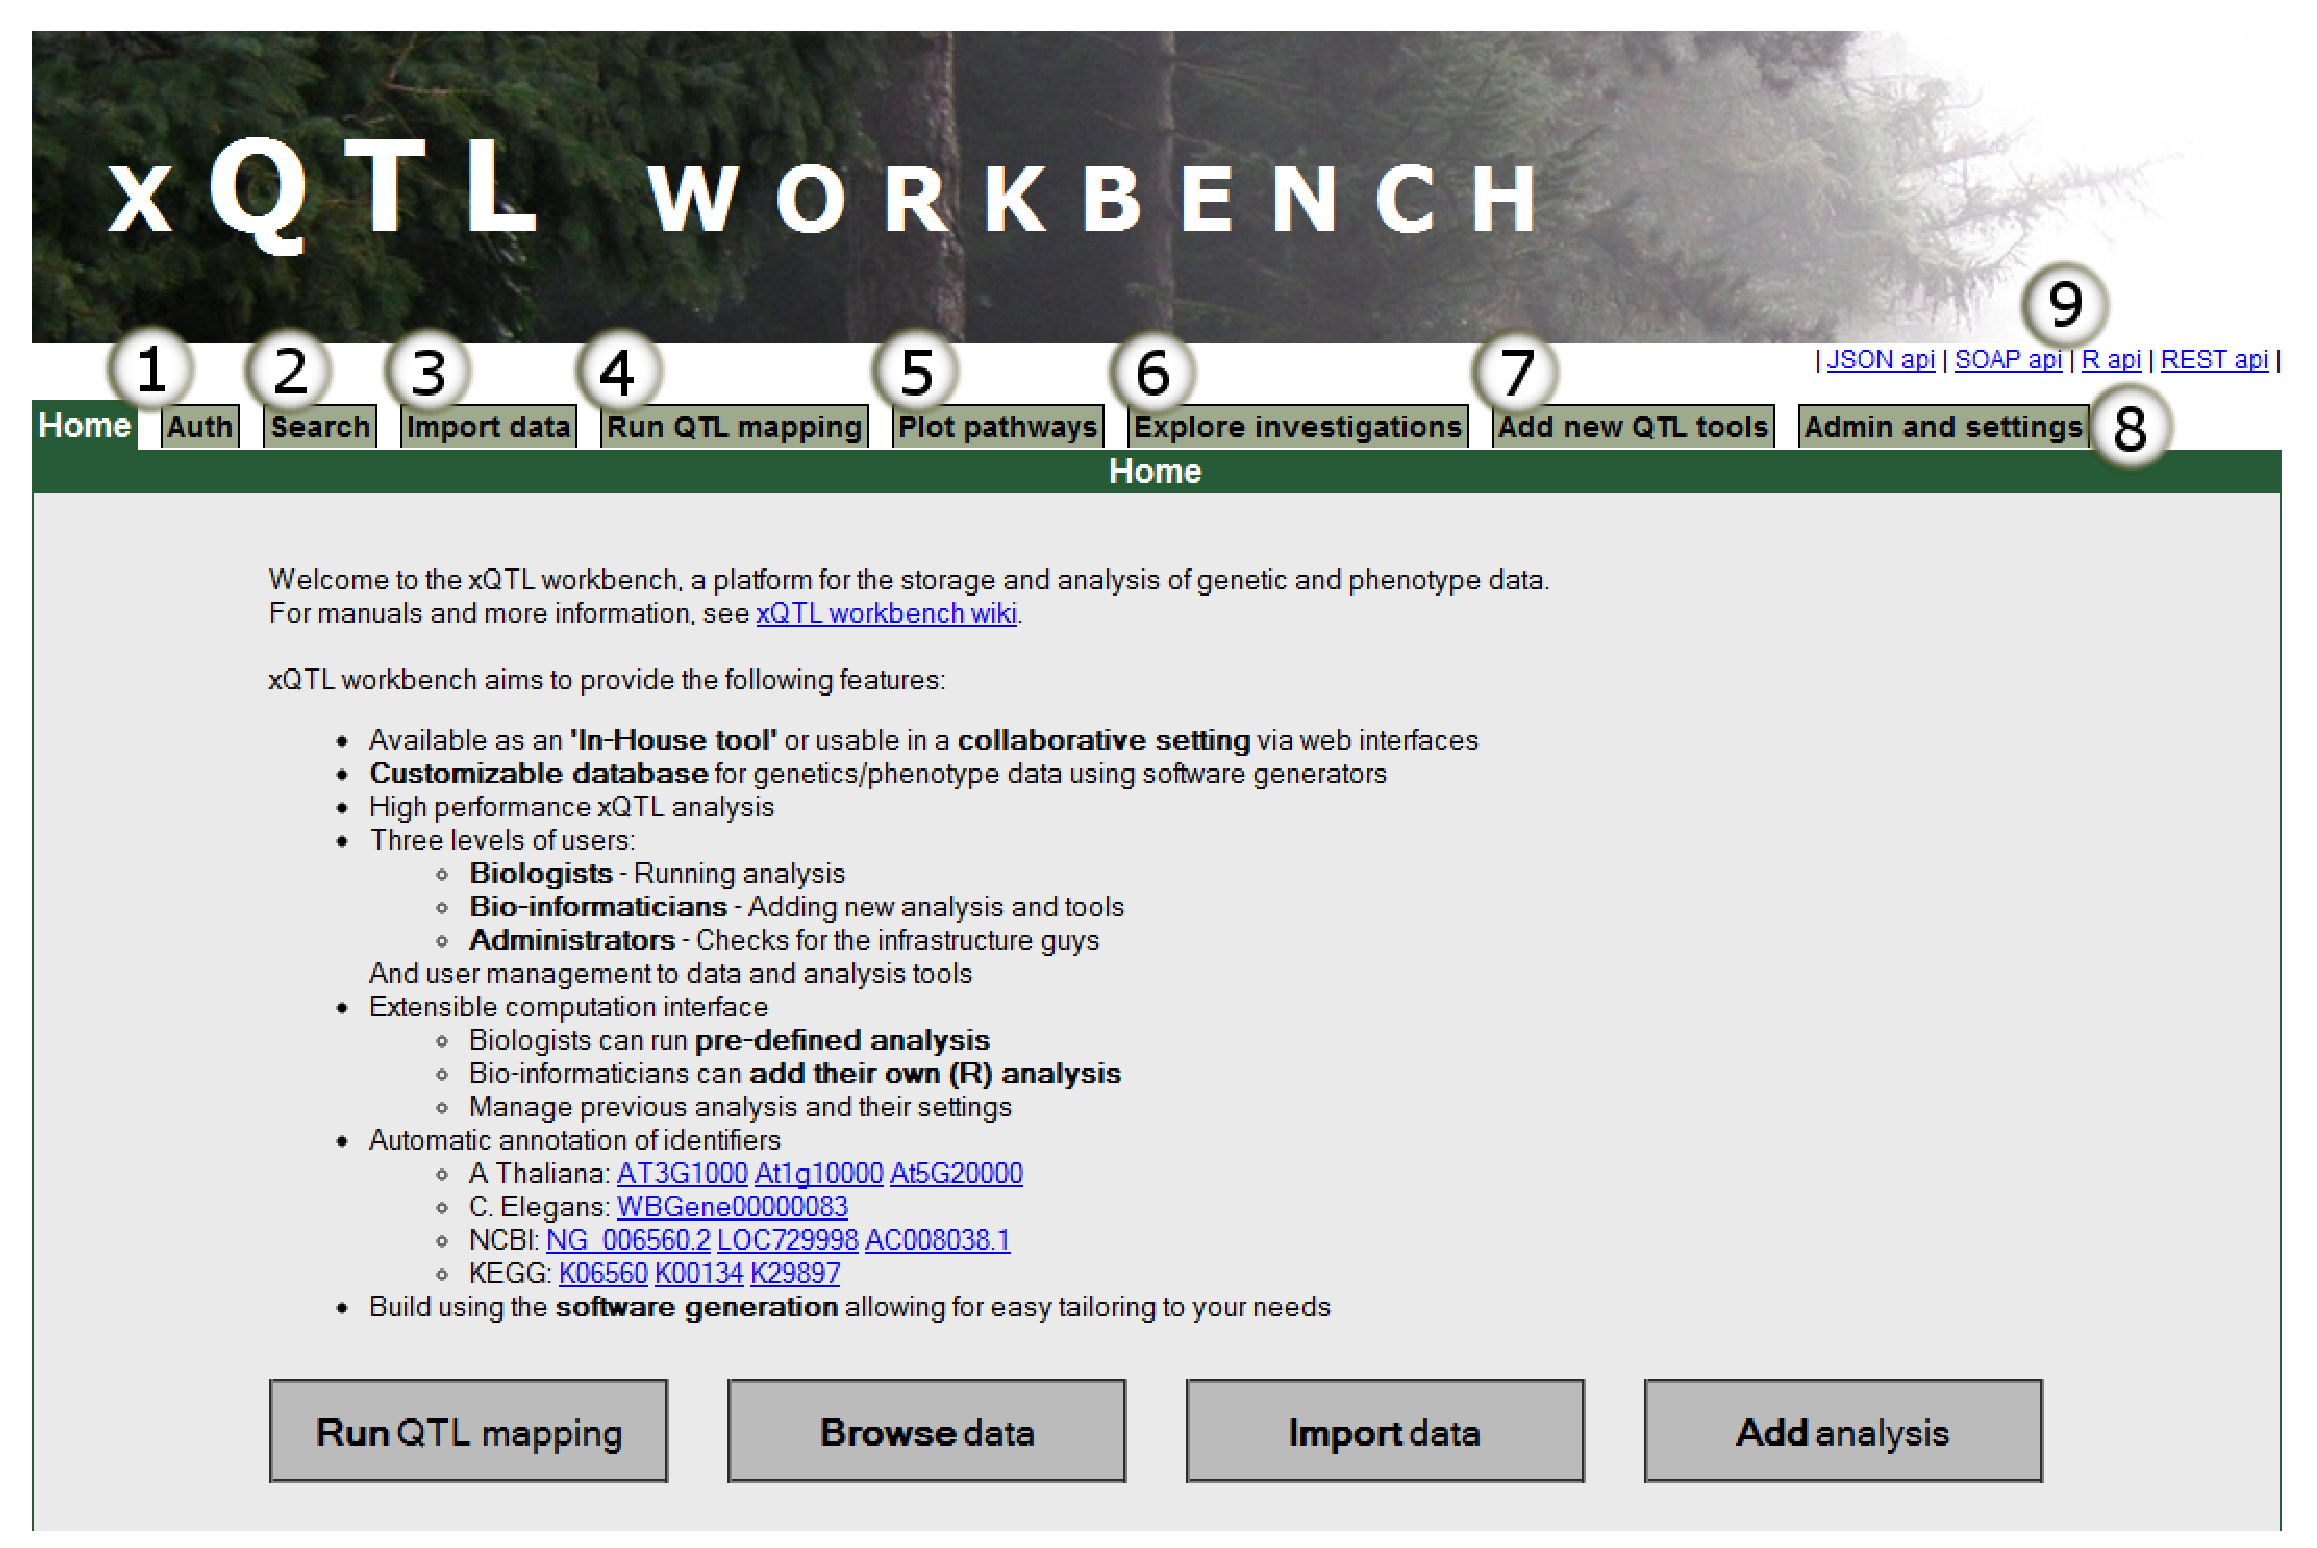
\includegraphics[width=0.81\textwidth]{eps/image_4_3.eps}
  \caption[XGAP.]
    {Experimental genotype and (molecular) phenotype data can be described using Subject, Trait, Data and DataElement; 
    the experimental procedures used can be described using Investigation, Protocol and ProtocolApplication (B). Specific 
    attributes and relationships can be added by extending core data types, e.g. Sample and Gene (A,C). The model is 
    described in UML: Arrows denote relationships (Data has a field Investigation that refers to Investigation ID); 
    Triangled lines denote inheritance (Metabolite inherits all properties ID, Name, Type from Trait, next to mass, 
    formula and structure); Triangled dotted lines denote use of interface (Spot 'implements' properties of Locus); 
    relationships are shown both as arrows and as properties ('xref' for one-to-many , 'mref' for many-to-many 
    relationships). Asterisk* marks FuGE derived types.}
    \label{fig:XGAP}
\end{figure}

We describe these biological components using FuGE data types and XGAP extensions thereof. 
Investigation binds all details of an investigation. Each investigation may apply a series 
of biomolecular \cite{Brown:2005} and computational \cite{Carey:2007,Alberts:2008,Fu:2007,Bhave:2007} 
Protocols. The applications of such Protocols are termed ProtocolApplications, which in the case 
of computational Protocols may require 
input Data and will deliver output Data.These data have the form of matrices, the DataElements 
of which have a row and a column index. Each row and column refers to a DimensionElement, 
being a particular Subject or a particular Trait, Table 2 illustrates the usage of these core 
data types. Figure \ref{fig:XGAP}a and \ref{fig:XGAP}c shows how the XGAP model can be extended to accommodate details on 
particular types of subjects and traits in a uniform way. A Trait can be a classical phenotype 
(for example, flowering - the flowering time is stored in the DataElement) or a biomolecular 
phenotype (for example, Gene X it's transcript abundance is stored in the DataElement). A 
Trait can also be a genotype (for example, Marker Y is a genomic feature observation that is 
stored in the DataElement). Genomic traits such as Gene, Marker and Probe all need additional 
information about their genome Locus to be provided. Similarly, a Subject can be a single 
Sample (for example, a labeled biomaterial as put on a microarray) and such a sample may 
originate from one particular Individual. It may also be a PairedSample when biomaterials come 
from two individuals - for example, if biomaterial has been pooled as in two-color microarrays. 
An individual belongs to a particular Strain. When new experiments are added new variants of 
Trait and Subject can be added in a similar way. Table 3 illustrates the generic usage of 
these extended data types.

Several standard data types were also inherited from FuGE to enable researchers to provide 
'Minimum Information' for QTLs and Association Studies such as defined in the MIQAS checklist 
 - a member of the Minimum Information for Biological and Biomedical Investigations (MIBBI) 
guideline effort \cite{Taylor:2008}

\subsection{Conclusions and Discussion}
In this paper we report a minimal and extensible data infrastructure for the management and 
exchange of genotype-to-phenotype experiments, including an object model for genotype and 
phenotype data (XGAP-OM), a simple file format to exchange data using this model (XGAP-TAB) 
and easy-to-customize database software (XGAP-DB) that will help groups to directly use and 
adapt XGAP as a platform for their particular experimental data and analysis protocols. We 
successfully evaluated the XGAP model and software in a broad range of experiments: array 
data (gene expression, including tiling arrays for detection of alternative splicing, 
ChIP-on-chip for methylation, and genotyping arrays for SNP detection); proteomics and 
metabolomics data (liquid chromatography time of flight mass spectrometry (LC-QTOF MS), NMR); 
classical phenotype assays \cite{Heap:2009, Bystrykh:2005, Li:2006, Keurentjes:2006, Stranger:2007, Bailey:2008, Beamer:1999}; 
other assays for detection of genetic markers; and annotation information for panel, gene, 
sample and clone. Non-technical partners successfully evaluated the practical utility by 
independently formatting and loading parts of their consortium data: EU-CASIMIR (for mouse), EU-GEN2PHEN (for human), 
EU-PANACEA (for \emph{C. elegans}) and IOP-Brassica (for plants). A public subset of these data sets 
is available for download at http://www.xgap.org. When needed we could quickly add customizations to the 
model, building on the general schema, and then use MOLGENIS to generate a new version of the 
software at the push of a button, for example, to support NMR methods as an extended type of 
Trait \cite{Fu:2009}. Furthermore we successfully integrated processing tools, such as a two-way 
communication with R/QTL \cite{Broman:2003, Arends:2010} enabling QTL mapping on XGAP 
stored genotypes and phenotypes with QTL results stored back into XGAP.

Based on these experiences, we expect use of XGAP to help the community of genome-to-phenome 
researchers to share data and tools, notwithstanding large variations in their research aims. 
The XGAP data format can be used to represent and exchange all raw, intermediate and result 
data associated with an investigation, and an XGAP database, for instance, can be used as a 
platform to share both data and computational protocols (for example, written in the R 
statistical language) associated with a research publication in an open format. We envision 
a directory service to which XGAP users can publish metadata on their investigations either 
manually or automatically by configuring this option in the XGAP administration user interface. 
This directory service can then be used as an entry point for federated querying between the 
community of XGAPs to share data and tools. Groups that already have an infrastructure can 
assimilate XGAP to ease evolution of their existing software.

Next to their existing user tools, they can 'rewire' algorithms and visual tools to also use 
the MOLGENIS APIs as data backend. Thus, researchers still have the same features as before, 
plus the features provided by the generated infrastructure (for example, data management GUIs, 
R/API) and connected tools (for example, R packages developed elsewhere). Moreover, much 
less software code needs to be maintained by hand when replacing hand-written parts by 
MOLGENIS-generated parts,  allowing software engineers to add new features for researchers 
much more rapidly. We invite the broader community to join our efforts at the public XGAP.org 
wiki, mailing list and source code versioning system to evolve and share the best XGAP 
customizations and GUI/API 'plug-in' enhancements, to support the growing range of profiling 
technologies, create data pipelines between repositories, and to push developments in the 
directions that will most benefit research

\section{High throughput data analysis (xQTL workbench)}
xQTL workbench is a scalable web platform for the mapping of quantitative trait loci (QTLs) 
at multiple levels: for example gene expression (eQTL), protein abundance (pQTL), metabolite 
abundance (mQTL) and phenotype (phQTL) data. Popular QTL mapping methods for model organism 
and human populations are accessible via the web user interface. Large calculations scale 
easily on to multi-core computers, clusters and Cloud. All data involved can be uploaded 
and queried online: markers, genotypes, microarrays, NGS, LC-MS, GC-MS, NMR, etc. When new 
data types come available, xQTL workbench is quickly customized using the MOLGENIS software 
generator.

Modern high throughput technologies generate large amounts of genomic, transcriptomic, proteomic, 
and metabolomic data. However, existing open source web-based tools for QTL analysis, such as 
webQTL \cite{Wang:2003} and QTLNetwork \cite{Yang:2008}, are not easily extendable to different 
settings and computationally scalable for whole genome analyses. \xqtlwb makes it easy to analyse 
large and complex datasets using state-of-the-art QTL mapping tools and to apply these methods 
to millions of phenotypes using paralellized 'Big Data' solutions\cite{Trelles:2011}. 
\xqtlwb also supports storing of raw, intermediate and final result data, and analysis protocols 
and history for reproducibility and data provenance. Use of MOLGENIS\cite{Swertz:2010b} 
helps to customize the software. All is conveniently accessible via standard Internet browsers on 
Windows, Linux or Mac (and using Java, R for the server).

\subsection{Features}
\xqtlwb provides visualization of QTL profiles, single and multiple QTL mapping methods, easy addition 
of new QTL analyses, scalable data management and analysis tracking.

\begin{figure}[h!]
  \centering
  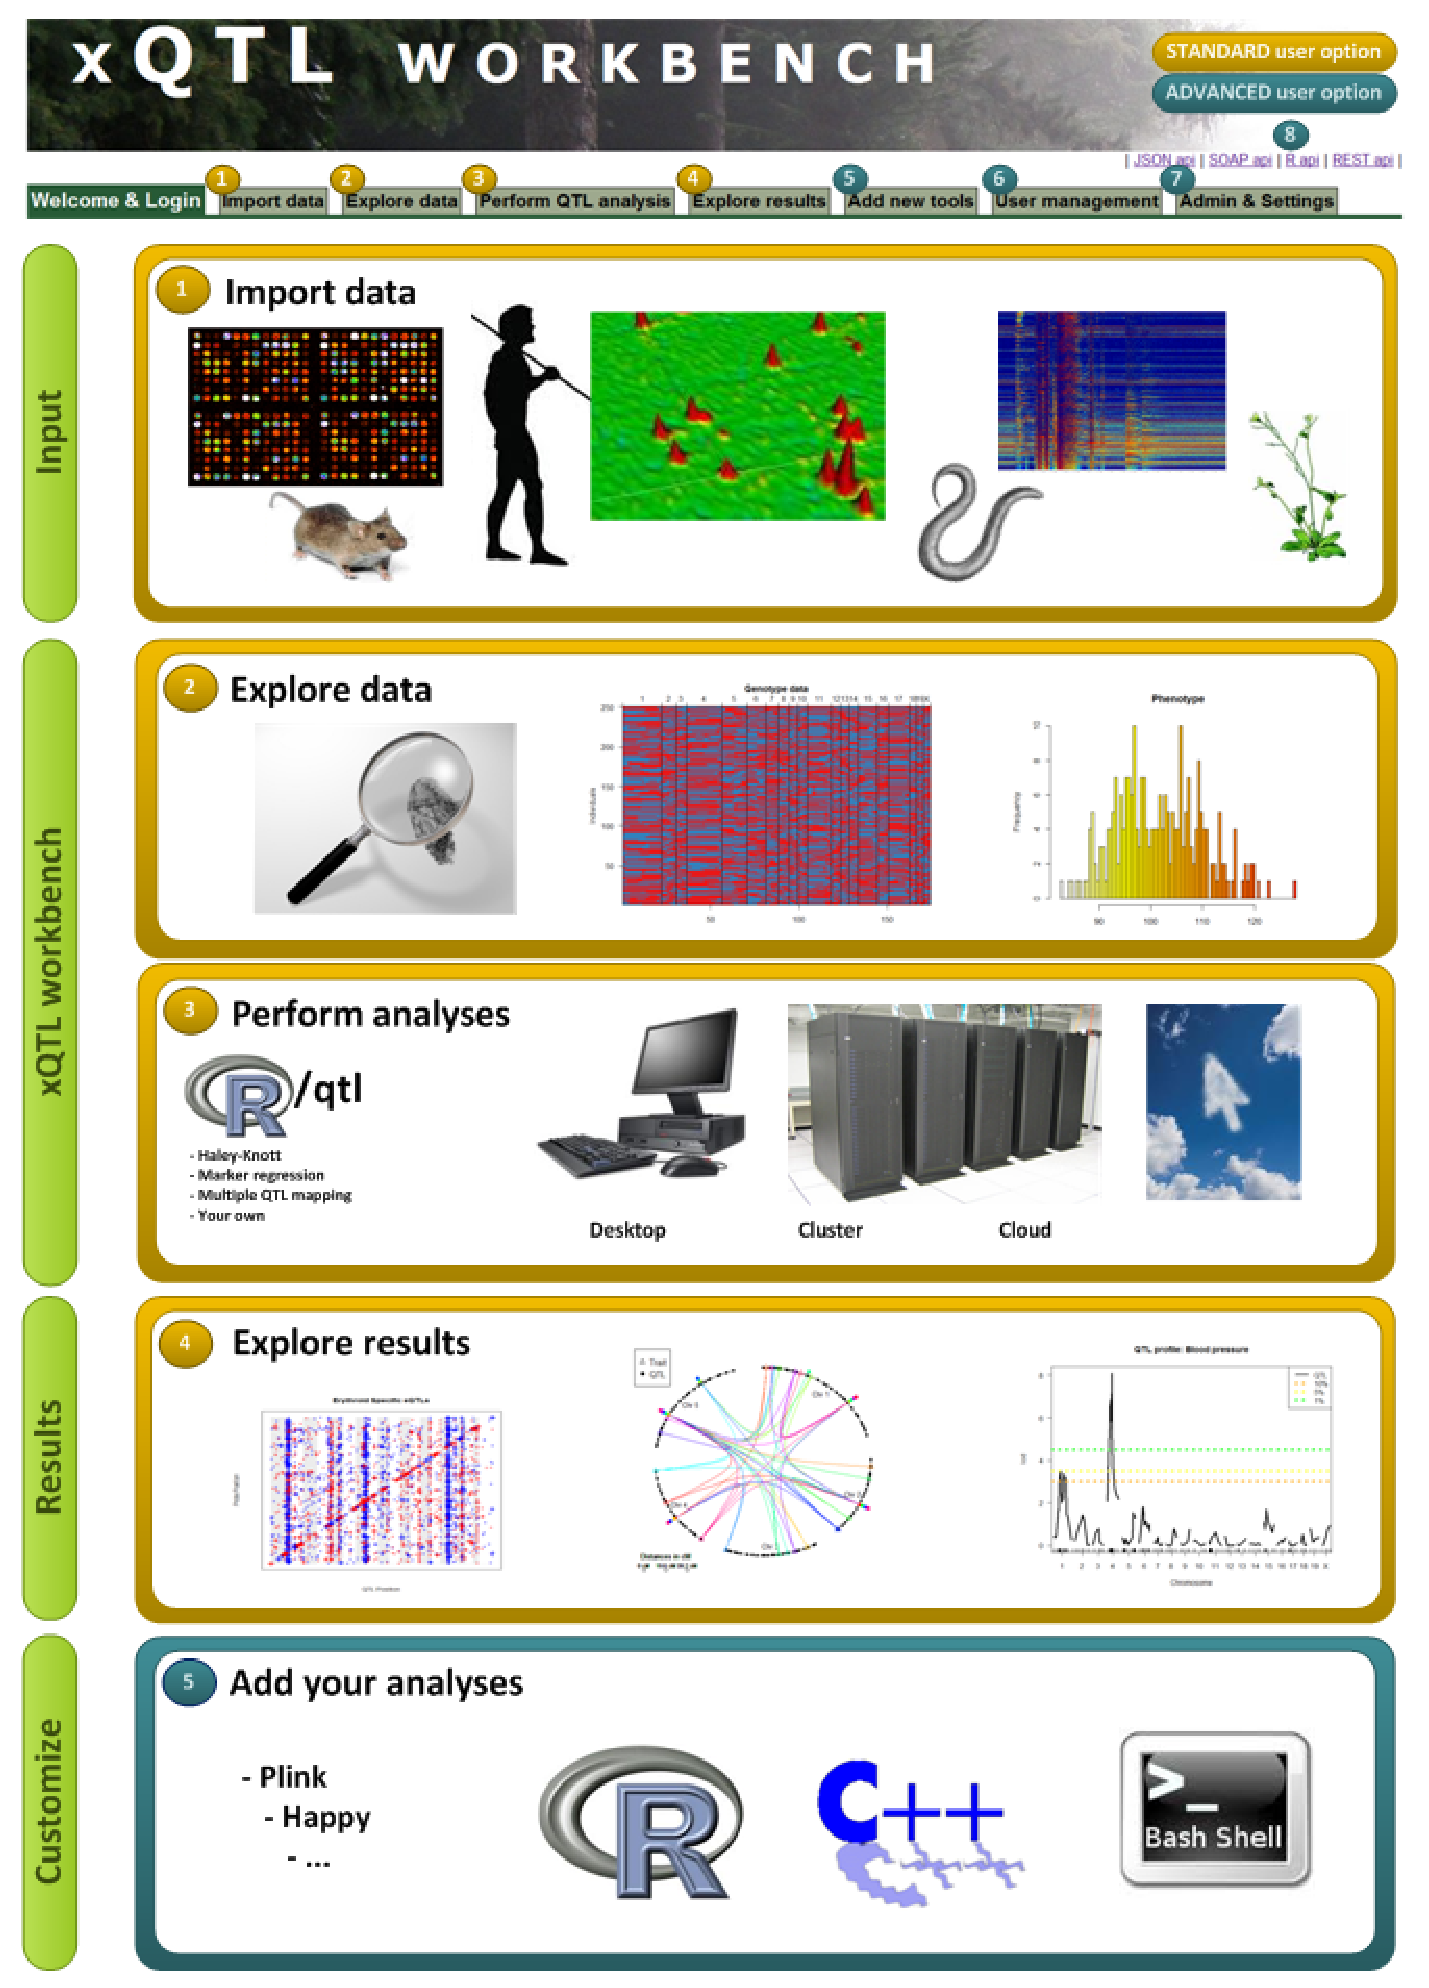
\includegraphics[width=0.75\textwidth]{eps/image_4_4.eps}
  \caption[xQTL workbench.]{Screenshot of xQTL workbench with all features enabled, (1) Import phenotype, genotype 
          and genetic map data, examples are given per import type; (2) Search through the whole database, explore 
          and browse your data using MOLGENIS generated web-interfaces; (3) Run R/qtl QTL mapping, the general 
          plugin allows users to perform not only QTL mapping but also other analyses; (4) Use default (or custom) 
          plugins to explore results (e.g. Heatmaps, QTL profiles); (5) Add new tools to the workbench (for 
          Bioinformaticians); (6) User management and access control of the system (Only for admins); (7) Expert 
          settings can be altered in the admin tab (Only for admins); (8) Connect/share data using generated API's 
          to R statistics, REST/JSON, SOAP.}
          \label{fig:xQTLworkbench}
\end{figure}

\begin{enumerate}\itemsep1pt
\item \emph{Explore QTL profiles} - Through the web-interface, users can explore mapped QTLs, and 
underlying information by viewing QTL plots in an interactive scrollable and zoomable window. 
\xqtlwb has support for other common image formats, such as PNG, JPG, SVG and embedded postscript; 
useful for publishing scientific results online, and on paper. From the output, main database identifiers, 
such as gene, protein and/or metabolite identifiers are automatically linked-out to matching external 
web pages of public database such as NCBI, KEGG, and Wormbase.
\item \emph{Single and multiple QTL mapping} - \xqtlwb wraps R/qtl \cite{Broman:2003, Arends:2010} in a 
web-based analysis framework offering all important QTL mapping routines, such as the EM algorithm, 
imputation, Haley-Knott regression, the extended Haley-Knott method, marker regression, and Multiple 
QTL mapping. In addition, \xqtlwb includes R/qtlbim, a library which provides a Bayesian model 
selection approach for mapping multiple interacting QTL \cite{Yandell:2007} and Plink, a library for 
association QTL mapping on Single Nucleotide Polymorphisms (SNP) in natural populations \cite{Purcell:2007}.
\item \emph{Add new analysis tools} - \xqtlwb supports flexible adding of more QTL analysis software: 
any R-based, or command-line tool, can be plugged in. All analysis results are uploaded, stored and 
tracked, in the \xqtlwb database through an R-API. When new tools are added, they can build on the 
high-level multi-core computer, cluster and Cloud management functions, based on TORQUE/OpenPBS and 
BioNode \cite{Prins:2012}. \xqtlwb can be made part of a larger analysis pipeline using interfaces to R, 
Excel, REST and SOAP web services and Galaxy \cite{Goecks:2010}.
\item \emph{Track and trace} - When a new analysis protocol or R script is defined, this protocol 
can easily be applied to new data. Also, \xqtlwb keeps track of history. Re-use of analysis protocols 
can be done in an automated fashion. Previous analyses can be rerun without resetting parameters. 
\xqtlwb provides an online overview of past analyses e.g. which analyses were performed, by who, when 
and display settings applied.
\item \emph{Scalable data management} - \xqtlwb has a consistency checking database based on XGAP 
specification \cite{Swertz:2010a}, user interfaces to manage and query genotype and phenotype data 
sets, and support for various database back-ends including HSQL (standalone) and MySQL. Phenotype, 
genotype and genetic map data can be imported as text (TXT), comma separated (CSV), and Excel files. 
\xqtlwb handles and stores large data in a new and efficient binary edition of the XGAP format, named 
XGAPbin (extension .xbin), documented online. Such binary formats are essential when handling, storing 
and transporting multi-Gigabyte datasets.
\item \emph{Customize to research} - Additional modules for new data modalities can be added using 
MOLGENIS software generator \cite{Swertz:2010b}. The 'look and feel' of \xqtlwb is adaptable to 
institute or consortium style by changing a simple template which is described in the \xqtlwb 
documentation enabeling seamless integration into an existing web-site or intranet site, such as 
recently for EU-PANACEA model organism project and LifeLines biobank.
\end{enumerate}

\subsection{Implementation}
We built \xqtlwb on top of MOLGENIS \cite{Swertz:2004}, a Java based software to generate tailored 
research infrastructure on-demand \cite{Swertz:2007}. From a single 'blueprint' describing the whole 
system, MOLGENIS auto-generates a full application including user interface, database infrastructure, 
application programming interfaces in R, REST and SOAP (APIs). MOLGENIS' flexibility and robustness 
is proven by the wide range of research projects, e.g. the Nordic GWAS Control database \cite{Leu:2010}, 
EB mutation database \cite{Akker:2011}, the Animal observation database \cite{Swertz:2010b}.

For data storage, the eXtensible Genotype and Phenotype (XGAP) data model was adopted \cite{Swertz:2010a} 
and extended for big data. To support the increased demand for computational resources for included 
mapping routines we added high-level cluster and cloud management functions for computation. The 
scalable QTL mapping routines of \xqtlwb are written in R and C. The choice of R ties in with the 
general practise of using R for QTL mapping. The user interface includes direct access to the R 
interpreter. Both \xqtlwb and MOLGENIS are open source software, and source code is transparently
stored and tracked in online source control repositories.

\subsection{Conclusions and Discussion}
\xqtlwb provides a total-solution for web-based analysis: Major QTL mapping routines are integrated 
for use by experienced and inexperienced users. Researchers can upload raw data, run analyses, explore 
mapped QTL and underlying information, and link-out to important databases. New algorithms can be 
flexibly added, immediately available to all users. Large analyses can be easily executed on a cluster, 
or in the Cloud. Future work include visualizations and search options to explore the results. We also 
had an EU-SYSGENET workshop that envisioned further integration of xQTL with analysis tools like HAPPY, 
databases like GeneNetwork, and the workflow manager TIQS \cite{Durrant:2012}.

\section{A worm database (WormQTL)}
WormQTL is one of the application developed using the xQTL workbench system. It is a public web portal 
for the management of all these new data and integrated development of suitable analysis tools. The 
web server provides a rich set of analysis tools available to use directly, based on R/qtl 
\cite{Broman:2003, Arends:2010}. Users can upload and share new R scripts as 'plugin' for colleagues 
in the community to use directly. New data can be uploaded and downloaded using XGAP-extensible 
text format for genotype and phenotypes\cite{Swertz:2010a}. All data and tools can be accessed 
via web user interfaces and programming interfaces to R, REST, and SOAP web services. Large 
consortia as well as individual researchers, can have a private area that is under embargo for 
publication. All software is free for download as MOLGENIS 'app' \cite{Swertz:2010b}. WormQTL is 
freely accessible without registration and is hosted on a large computational cluster enabling 
high throughput analyses to all at http://www.wormqtl.org.

\subsection{Background}

Over the past 30 years, the metazoan \emph{Caenorhabditis elegans} has become a premier animal model for 
determining the genetic basis of quantitative traits \cite{Gaertner:2010, Kammenga:2008}. The 
extensive knowledge of molecular, cellular and neural bases of complex phenotypes makes 
\emph{C. elegans} an ideal system for the next endeavour: determining the role of natural genetic 
variation on system variation. These efforts have resulted in an accumulation of a valuable amount 
of phenotypic, high-throughput molecular and genotypic data across different developmental worm 
stages and environments in hundreds of strains \cite{Palopoli:2008, Kammenga:2007, Rockman:2010, 
McGrath:2009, Reddy:2009, Doroszuk:2009, Li:2010, Gutteling:2007, Vinuela:2010}. In addition, a similar wealth has been 
produced on hundreds of different \emph{C. elegans} wild isolates and other species \cite{Andersen:2012}. 
For example, \emph{C. briggsae} is an emerging model organism that allows evolutionary comparisons 
with \emph{C. elegans} and quantitative genetic exploration of its own unique biological 
attributes \cite{Ross:2011}.

This rapid increase in valuable data calls for an easily accessible database allowing for 
comparative analysis and meta-analysis within and across Caenorhabditis species \cite{Swertz:2007}. To 
facilitate this, we designed a public database repository for the worm community, WormQTL 
(http://www.wormqtl.org). Driven by the PANACEA project of the systems biology program of 
the EU, its design was tuned to the needs of \emph{C. elegans} researchers via an intensive 
series of interactive design and user evaluation sessions on a mission to integrate all 
available data within the project.

As a result, data that were scattered across different platforms and databases can now be 
stored, downloaded, analysed and visualized in an easily and comprehensive way in WormQTL. 
On top, the database provides a set of user interfaced analysis tools to search the database 
and explore genotype-phenotype mapping based on R/qtl \cite{Broman:2003, Arends:2010}. New 
data can be uploaded and downloaded using the extensible plain text format for genotype and 
phenotypes, XGAP \cite{Swertz:2010a}. There is no limit to the type of data (from gene 
expression to protein, metabolite or cellular data) that can be accommodated because of its 
extensible design. All data and tools can be accessed via a public web user interface and 
programming interfaces to R and REST web services, which were built using the MOLGENIS 
biosoftware toolkit \cite{Swertz:2010b}. Moreover, users can upload and share more R 
scripts as 'plugin' for the colleagues in the community to use directly and run those on a 
computer cluster using software modules from xQTL workbench \cite{Arends:2012, Snoek:2012}; this requires 
login to prevent abuse. All software can be downloaded for free to be used, for example as 
local mirror of the database, and/or to host new studies.

All the software was built as open source, reusing and building on existing open source components 
as much as possible. WormQTL is freely accessible without registration and is hosted on a large 
computational cluster enabling high-throughput analyses at http://www.wormqtl.org. Below we detail 
the results, methods used to implement the system and future plans.

\subsection{Results}
WormQTL is an online database platform for expression quantitative trait loci (eQTL) exploration 
to service the worm community and already provides many publicly available data sets \cite{Rockman:2010, 
Doroszuk:2009, Li:2006, Li:2010, Gutteling:2007, Vinuela:2010, Elvin:2011, Vinuela:2012}. New data 
sets can be uploaded using the XGAP plain file data format. Suitable help pages are provided. 
Currently, 38 public data sets have been loaded, of which the bulk is xQTL data on 500 strains 
(introgression lines, recombinant inbred lines (RILs), recombinant inbred advanced intercross lines 
and natural isolates), 55,000 transcripts, 1594 samples and 1579 markers (Table 1). With this 
combination of classical phenotypes, molecular profiles and genetics data sets, WormQTL contains 
all the 'genetical genomics' experiments published to our current knowledge (except for some tiling 
data). Using WormQTL, researchers can explore many xQTLs across the various studies in different 
conditions and ages and compare classical QTLs with xQTLs. The main interfaces are 'Find QTLs', 
'Genome browser' and 'Browse data'.

\begin{enumerate}\itemsep1pt
\item \emph{Find QTLs} - QTL is genomic regions associated with phenotypic variation and can be 
used to study the genetic architecture of traits and to detect potential phenotypic regulators. 
Recently, the number of QTLs and especially eQTL studies in \emph{C. elegans} has increased greatly. 
These eQTL studies consist of large data sets that, before WormQTL, were very difficult to access 
and perform a combined meta-analysis. Therefore, we provide easy access to most of the eQTL studies 
published, by search, browse and plot functions (Figure \ref{fig:xQTLworkbench}). We support relatively simple questions like 
'does my gene have an xQTL?' to more advanced ones like 'how do these genes fit into an xQTL network?'. 
All the matching genes, markers and traits found in the data sets are returned including links to 
WormBase and literature. Furthermore, WormQTL is the first portal for any species that allows comparison 
of eQTLs over multiple experiments and environments, giving insight in the plastic nature of genetic 
regulation.
\item \emph{Genome browser} - To find the genes that have a QTL on your favourite position, click 
'Genome browser'. Here, you can select from all the different releases of the University of California, 
Santa Cruz genome releases. You can add tracks from the designated experiments of interest. Then 
navigate to your favourite location (tip: use open in new window) and collect significant probe 
identifiers from that region.
\item \emph{Browse data} - Complete data sets and accompanying gene, sample and trait identifier 
lists can be browsed via the 'browse data' user interface. External identifiers anywhere in the 
data are automatically recognized and enhanced as linkouts to background information, such as links 
to Wormbase, NCBI, KEGG or Ensembl. All the annotation lists and data matrices can be browsed and 
searched in a tabular form and can be downloaded as plain text or Excel files. Readers can also 
download data sets or submit new data sets using the XGAP data format following examples described 
in the WormQTL help section. Also all data can be accessed programmatically from with R (as whole 
matrix or per row) or using REST web services, including filtering of the annotations (genes, probes, 
markers and phenotypes) and services to 'slice' individual lines out of the complete data sets to 
speed up download and (parallel) analyses. Alternatively, readers can request a login to upload 
data and new analysis scripts directly.
\end{enumerate}

\subsection{Conclusions and Discussion}
\subsubsection{Implementation}
All the software was implemented using the open source Molecular Genetics Information Systems 
MOLGENIS toolkit \cite{Swertz:2010a}, and in particular one previously existing MOLGENIS application, the 
extensible xQTL workbench \cite{Arends:2012} and the R/qtl QTL mapping and visualization package for the R 
language \cite{Broman:2003, Arends:2010}. The MOLGENIS toolkit is a Java-based software to generate tailored research 
infrastructure on demand \cite{Swertz:2007}. From a single 'blueprint' describing all biological data 
structures and user interfaces of the whole system, MOLGENIS autogenerates a full application 
including user interface, database infrastructure and application programming interfaces 
(APIs) in R, REST and SOAP.

At the push of a button, MOLGENIS 'generators' automatically translates these models into a 
database, standard user interfaces for data queries and updates, upload/download tools for 
tab-delimited data and scriptable interfaces for programmers to users from within R and via 
web services. This greatly speeded up the initial software development and also enables rapid 
extension when, for example, new data types arrive. On top of this foundation, we build the 
WormQTL specific user interactions such as the 'Find QTLs' and the 'Genome browser' using 
MOLGENIS 'plug-in' mechanism and the visualizations and plots using the R interface. xQTL 
workbench is a scalable web platform for the mapping of QTLs at multiple levels: for example, 
gene expression (xQTL), protein abundance (pQTL), metabolite abundance (mQTL) and phenotype 
(phQTL) data. The xQTL workbench provided a set of previously developed user interfaces to 
run R/qtl mapping methods directly from within the WormQTL user interface, the ability to 
add new analysis procedures in R, data management and data format conversions, all greatly 
speeding up the generation of new xQTL profiles.

All the data sets were downloaded from their original sources and then formatted using the 
XGAP data format. XGAP is a simple text file format that uses a directory of tab-delimited 
files or one Excel file with multiple sheets to load lists of annotations and data matrices. 
The annotations list all the background information needed to run and interpret the analysis 
including, for example, genome position information, such as markers, genes, probes and 
strains. The data matrices describe all the raw, intermediate and result data, such as gene 
expression, genotypes and QTL P-values, with the row names and column names cross linking to 
the annotations. For example, gene expression is a matrix of 'gene' X 'sample'. Subsequently 
these data sets were loaded using the MOLGENIS/xQTL data import wizards, which check the 
files for correctness and give informative feedback if the data are not yet in a format that 
WormQTL can understand \cite{Swertz:2010a}. All the annotations are stored in tables in the database; the 
large data matrices are stored in a optimized binary format to speed up analyses and queries. 
This format is documented in the WormQTL manual to ease the submission of new data sets from 
the community. Finally, all the QTL profiles were recalculated according to the specification 
of the original, or slightly modified when needed, such as to include a previously missing 
wrongly labelled sample correction. In this process, we greatly benefitted from the integration 
with xQTL workbench, which enabled us to re-run all these analyses on the computer cluster 
and add new R analysis procedures when needed, simply from the user interface.

All software is available as open source on http://github.com/molgenis for others to reuse 
locally, and related technical documentation is available at http://www.xqtl.org and 
http://www.rqtl.org and http://www.molgenis.org.

\subsubsection{Future plans}
The current version of WormQTL (June 2012) is a comprehensive, versatile and flexible package. 
Follow-up plans of more extended versions with new tools and data depend on the demand by the 
users of WormQTL. We envisage that in the future, three types of new tools will be developed: 
(i) visualization tools, (ii) QTL mapping tools and (iii) candidate gene selection tools. Improved 
visualization tools might include plotting a phenotype against the marker at a certain position; 
so the two groups become visible at a QTL position. Also plots can be made showing transgression 
and heritability per microarray probe or gene or histograms of the phenotypic values (and include 
the parental values if available). Advanced QTL mapping tools might include multi-environment
/age mapping or genotype-by-environment analyses, developed in collaboration with the R/qtl team 
to enable automatic links to this software. The candidate gene selection tools would benefit from 
the most recent stable release of Wormbase \cite{Yook:2012}, the most widely used platform for worm biology. 
But also other sources of information like MODENCODE \cite{Gerstein:2010} or Wormnet 
\cite{Lee:2008} are likely to be connected with WormQTL. A candidate gene selection tool might be 
implemented in a next version 
of WormQTL as it is less easy to implement and often needs information beyond WormQTL. One can 
think of (i) which SNPs/genes/polymorphic genes/transcription factor binding sites and so forth 
are underlying a eQTL; (ii) which gene, underlying my xQTL, is linked to most of the genes 
having an xQTL; (iii) which genes are polymorphic and (iv) which other genotypes show a difference 
in expression and do they share polymorphisms with the parental strains of the RIL population 
that the xQTL was mapped in. Moreover, WormQTL can be easily expanded to other Caenorhabditis 
species \cite{Ross:2011}.

We believe that WormQTL, which will be continuously curated by the members of this international 
consortium, is a very attractive database for the growing community of quantitative genetics in 
worms researchers. We are committed to maintain data and software for the years to come and invite 
the community to add and share new data and ideas.



\chapter{High throughput infrastructure for system genetics}
\thispagestyle{empty}
\label{chap:xqtlwormbench}

\emph{Modern high-throughput technologies generate large amounts of genomic, transcriptomic, 
proteomic and metabolomic data, creating a major challenge in bioinformatics from the size 
of data collected and the multitude of technologies used. We present the xQTL workbench 
system \cite{Arends:2012}, a flexible and scalable platform to store and analyse all these 
new phenotype and genotype data using XGAP \cite{Swertz:2010a} dataformat and MOLGENIS software 
\cite{Swertz:2004}. We evaluated the system in multiple applications of which WormQTL database 
\cite{Snoek:2012} is presented here.}

\null
\vfill

\begin{myexampleblock}{Originally published as:}
  \authors{Morris A Swertz, Martijn Dijkstra, ..., Danny Arends, George Byelas, et al}\\
  \emph{The MOLGENIS toolkit: rapid prototyping of biosoftware at the push of a button}\\
  \bold{BMC Bioinformatics} (2010)\\\\

  \authors{Morris A Swertz, K Joeri v/d Velde, Bruno M Tesson, ..., Danny Arends, et al}\\
  \emph{XGAP: a uniform and extensible data model and software platform for genotype and phenotype experiments}\\
  \bold{Genome Biology} (2010)\\\\

  \authors{Danny Arends*, K. Joeri v/d Velde*, Pjotr Prins, Karl W. Broman, et al.}\\
  \emph{xQTL workbench: a scalable web environment for multi-level QTL analysis}\\
  \bold{Bioinformatics} (2012)\\\\

  \authors{Danny Arends*, L. Basten Snoek*, Joeri v/d Velde*, Yang Li*, et al.}\\
  \emph{WormQTL: Public archive and analysis web portal for natural variation data in Caenorhabditis spp}\\
  \bold{Nucleic Acids Research} (2012)
\end{myexampleblock}

\newpage

\begin{wrapfigure}{r}{0.5\textwidth}
  \centering
  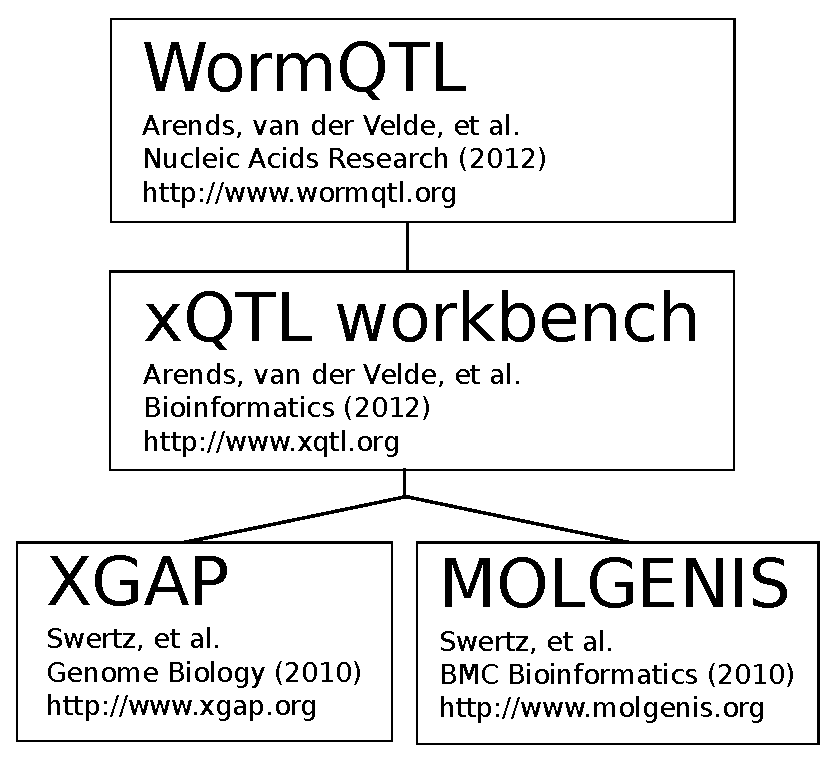
\includegraphics[width=0.4\textwidth]{eps/image_5_0.eps}
  \caption[Overview]
    {Overview of this chapter and how the different parts of this chapter are related to eachother.}
    \label{fig:Overview}
\end{wrapfigure}

Modern genetic and genomic technologies provide researchers with unprecedented amounts of raw and processed 
data and the need for software infrastructures to manage and process the large datasets produced is widely 
accepted \cite{Swertz:2004, Stein:2008, Thorisson:2009}. For example, recent genetical genomics 
\cite{Swertz:2004, Stein:2008, Thorisson:2009} studies have mapped gene expression (eQTL), 
protein abundance (pQTL) and metabolite abundance (mQTL) to genetic variation using genome-wide linkage and 
genome-wide association experiments on various microarray, mass spectrometry and proton nuclear magnetic 
resonance (NMR) platforms and in a wide range of organisms, including human \cite{Goring:2007, Tanaka:2009, 
Heap:2009}, yeast \cite{Brem:2002, Brem:2005}, mouse \cite{Bystrykh:2005}, rat \cite{Ramos:1999}, 
\emph{Caenorhabditis elegans} \cite{Li:2010} and \emph{Arabidopsis thaliana} \cite{Keurentjes:2006, Keurentjes:2007, Fu:2009}.

Understanding these and other high-tech genotype-to-phenotype data is challenging and depends on suitable 
'cyber infrastructure' to integrate and analyze data \cite{Stein:2008, Fay:2008}: data infrastructures to store and query the 
data from different organisms, biomolecular profiling technologies, analysis protocols and experimental 
designs; graphical user interfaces (GUIs) to submit, trace and retrieve these particular data; communicating 
infrastructure in, for example, R \cite{Ihaka:1996}, Java and web services to connect to different processing infrastructures 
for statistical analysis \cite{Alberts:2008, Fu:2007} and/or integration of background information from public 
databases \cite{Smedley:2008}; and a simple file format to load and exchange data within and between projects.

Many elements of the required cyber infrastructure are available: The Generic Model Organism Database (GMOD) 
community developed the Chado schema for sequence, expression and phenotype data \cite{Mungall:2007, OConnor:2008} and delivered reusable 
software components like gbrowse \cite{Stein:2002}; the BioConductor community has produced many analysis packages that 
include data structures for particular profiling technologies and experimental protocols \cite{Gentleman:2004}. 

Some integrated cyber infrastructures are also available: the National Center for Biotechnology Information (NCBI) 
has launched dbGaP (database of genotypes and phenotypes) \cite{Mailman:2007}, a public database to archive genotype 
and clinical phenotype data from human studies; and the Complex Trait Consortium has launched GeneNetwork \cite{GeneNetwork:2004}, 
a database for mouse genotype, classical phenotype and gene expression phenotype data with tools for 'per-trait' quantitative trait loci (QTL) analysis.

However, a suitable and customizable integration of these elements to support high throughput genotype-to-phenotype 
experiments is still needed \cite{Thorisson:2009}: dbGaP, GeneNetwork and the model organism databases are designed 
as international repositories and not to serve as general data infrastructure for individual projects; many of the 
existing bespoke data models are too complicated and specialized, hard to integrate between profiling technologies, 
or lack software support to easily connect to new analysis tools; and customization of the existing infrastructures 
dbGaP, GeneNetwork or other international repositories \cite{Zeng:2007, Hu:2007} or assembly of Bioconductor and 
generic model organism database components to suit particular experimental designs, organisms and biotechnologies 
still requires many minor and sometimes major manual changes in the software code that go beyond what individual 
lab bioinformaticians can or should do, and result in duplicated efforts between labs if attempted. Existing open 
source web-based tools for QTL analysis, such as webQTL \cite{Chesler:2004} and QTLNetwork \cite{Yang:2008}, are 
not easily extendable to different settings and computationally scalable for whole genome analyses.

We here present xQTL workbench and its application in the WormQTL database. WormQTL (http://www.wormqtl.org) is an 
easily accessible database enabling search, comparative analysis and meta-analysis of all data on variation in \emph{Caenorhabditis spp}.
All was built on top of xQTL workbench, a generic scalable web platform for the mapping of quantitative trait loci (QTLs)
 at multiple levels: for example gene expression (eQTL), protein abundance (pQTL), metabolite abundance (mQTL) and phenotype 
(phQTL) data. xQTL workbench supports storing of raw, intermediate and final result data, and analysis protocols and history 
for reproducibility and data provenance using XGAP data model \cite{Swertz:2010a}. Use of Molgenis \cite{Swertz:2010b} helped 
to build and customize the software. All is conveniently accessible via standard Internet browsers on Windows, Linux or Mac 
(and using Java, R for the server). xQTL workbench, MOLGENIS, XGAP and WormQTL are related to eachother as outlined in 
Figure \ref{fig:Overview}, and.are described in detail below.

\section{High throughput data analysis (xQTL workbench)}
Existing open source web-based tools for QTL analysis, such as webQTL \cite{Wang:2003, Chesler:2004} and 
QTLNetwork \cite{Yang:2008}, are not easily extendable to different settings and computationally 
scalable for whole genome analyses. \xqtlwb makes it easy to analyse large and complex 
datasets using state-of-the-art QTL mapping tools and to apply these methods to millions of 
phenotypes using parallelized 'Big Data' solutions \cite{Trelles:2011}.
\xqtlwb also supports storing of raw, intermediate and final result data, and analysis protocols 
and history for reproducibility and data provenance. Use of MOLGENIS\cite{Swertz:2010b} 
helps to customize the software. All is conveniently accessible via standard Internet browsers on 
Windows, Linux or Mac (and using Java, R for the server).

xQTL workbench is a scalable web platform for the mapping of quantitative trait loci (QTLs) 
at multiple levels: for example gene expression (eQTL), protein abundance (pQTL), metabolite 
abundance (mQTL) and phenotype (phQTL) data. Popular QTL mapping methods for model organism 
and human populations are accessible via the web user interface. Large calculations scale 
easily on to multi-core computers, clusters and Cloud. All data involved can be uploaded 
and queried online: markers, genotypes, microarrays, NGS, LC-MS, GC-MS, NMR, etc. When new 
data types come available, xQTL workbench is quickly customized using the MOLGENIS software 
generator. xQTL workbench provides visualization of QTL profiles, single and multiple QTL 
mapping methods, easy addition of new QTL analyses, scalable data management and analysis 
tracking, described below:

\subsection{Features}
\xqtlwb provides visualization of QTL profiles, single and multiple QTL mapping methods, easy addition 
of new QTL analyses, scalable data management and analysis tracking.

\begin{figure}[h!]
  \centering
  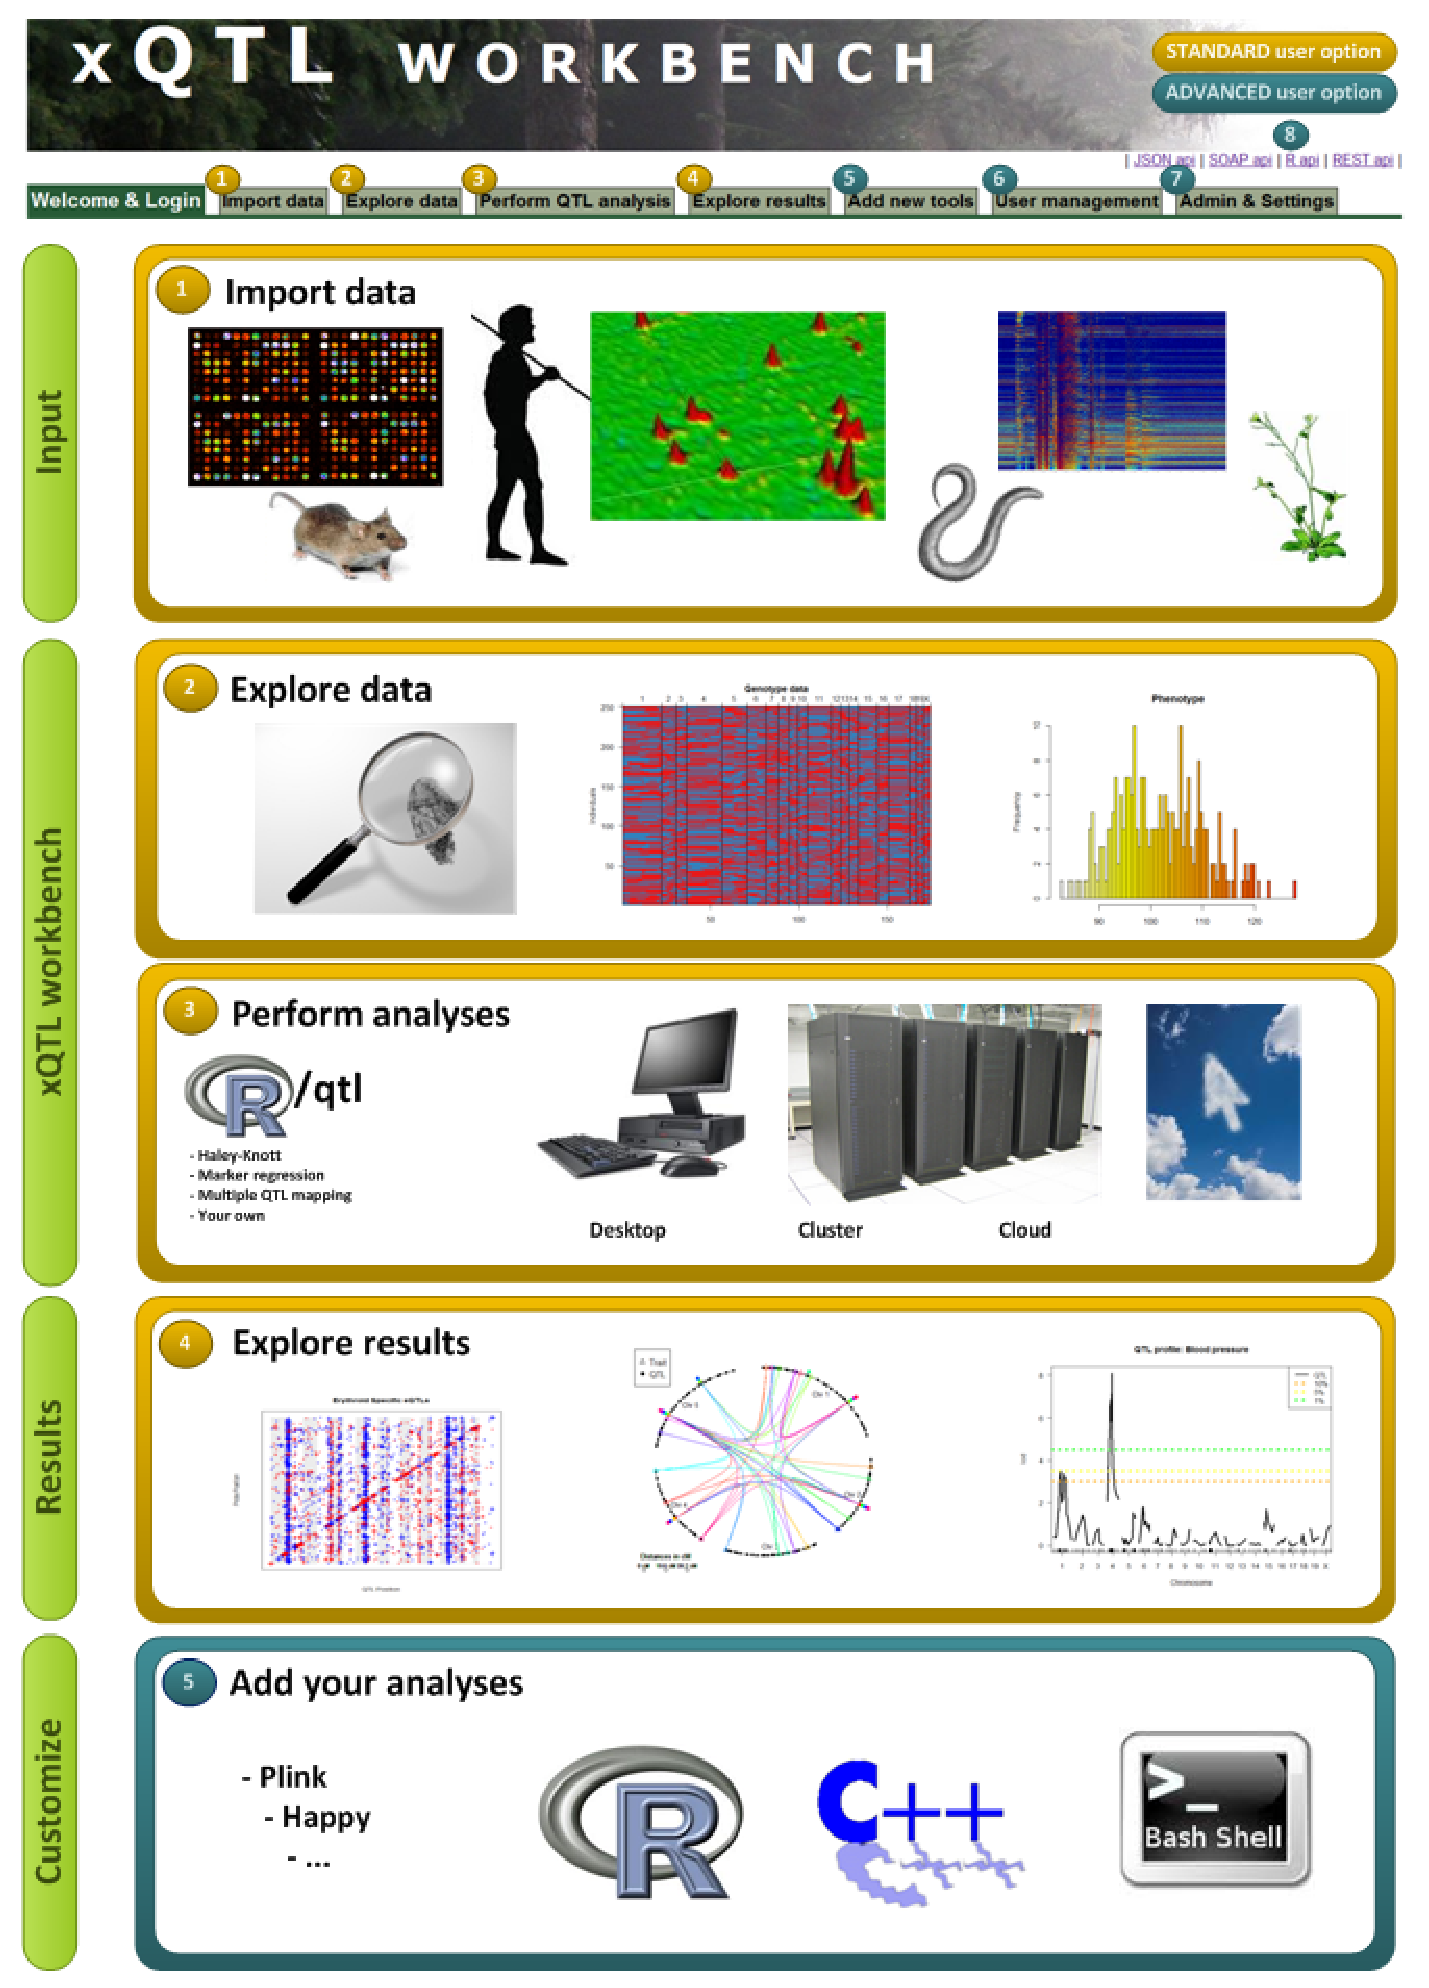
\includegraphics[width=0.75\textwidth]{eps/image_5_4.eps}
  \caption[xQTL workbench.]{Screenshot of xQTL workbench with all features enabled, (1) Import phenotype, genotype 
          and genetic map data, examples are given per import type; (2) Search through the whole database, explore 
          and browse your data using MOLGENIS generated web-interfaces; (3) Run R/qtl QTL mapping, the general 
          plugin allows users to perform not only QTL mapping but also other analyses; (4) Use default (or custom) 
          plugins to explore results (e.g. Heatmaps, QTL profiles); (5) Add new tools to the workbench (for 
          Bioinformaticians); (6) User management and access control of the system (Only for admins); (7) Expert 
          settings can be altered in the admin tab (Only for admins); (8) Connect/share data using generated API's 
          to R statistics, REST/JSON, SOAP.}
          \label{fig:xQTLworkbench}
\end{figure}

\begin{enumerate}\itemsep1pt
\item \emph{Explore QTL profiles} - Through the web-interface, users can explore mapped QTLs, and 
underlying information by viewing QTL plots in an interactive scrollable and zoomable window. 
\xqtlwb has support for other common image formats, such as PNG, JPG, SVG and embedded postscript; 
useful for publishing scientific results online, and on paper. From the output, main database identifiers, 
such as gene, protein and/or metabolite identifiers are automatically linked-out to matching external 
web pages of public database such as NCBI, KEGG, and Wormbase.
\item \emph{Single and multiple QTL mapping} - \xqtlwb wraps R/qtl \cite{Broman:2003, Arends:2010} in a 
web-based analysis framework offering all important QTL mapping routines, such as the EM algorithm, 
imputation, Haley-Knott regression, the extended Haley-Knott method, marker regression, and Multiple 
QTL mapping. In addition, \xqtlwb includes R/qtlbim, a library which provides a Bayesian model 
selection approach for mapping multiple interacting QTL \cite{Yandell:2007} and Plink, a library for 
association QTL mapping on Single Nucleotide Polymorphisms (SNP) in natural populations \cite{Purcell:2007}.
\item \emph{Add new analysis tools} - \xqtlwb supports flexible adding of more QTL analysis software: 
any R-based, or command-line tool, can be plugged in. All analysis results are uploaded, stored and 
tracked, in the \xqtlwb database through an R-API. When new tools are added, they can build on the 
high-level multi-core computer, cluster and Cloud management functions, based on TORQUE/OpenPBS and 
BioNode \cite{Prins:2012}. \xqtlwb can be made part of a larger analysis pipeline using interfaces to R, 
Excel, REST and SOAP web services and Galaxy \cite{Goecks:2010}.
\item \emph{Track and trace} - When a new analysis protocol or R script is defined, this protocol 
can easily be applied to new data. Also, \xqtlwb keeps track of history. Re-use of analysis protocols 
can be done in an automated fashion. Previous analyses can be rerun without resetting parameters. 
\xqtlwb provides an online overview of past analyses e.g. which analyses were performed, by who, when 
and display settings applied.
\item \emph{Scalable data management} - \xqtlwb has a consistency checking database based on XGAP 
specification \cite{Swertz:2010a}, user interfaces to manage and query genotype and phenotype data 
sets, and support for various database back-ends including HSQL (standalone) and MySQL. Phenotype, 
genotype and genetic map data can be imported as text (TXT), comma separated (CSV), and Excel files. 
\xqtlwb handles and stores large data in a new and efficient binary edition of the XGAP format, named 
XGAPbin (extension .xbin), documented online. Such binary formats are essential when handling, storing 
and transporting multi-Gigabyte datasets.
\item \emph{Customize to research} - Additional modules for new data modalities can be added using 
MOLGENIS software generator \cite{Swertz:2010b}. The 'look and feel' of \xqtlwb is adaptable to 
institute or consortium style by changing a simple template which is described in the \xqtlwb 
documentation enabling seamless integration into an existing web-site or intranet site, such as 
recently for EU-PANACEA model organism project and LifeLines biobank.
\end{enumerate}

\subsection{Reusable software (MOLGENIS)}
\subsubsection{Background}
High throughput technologies have boosted biological and medical research and the need for software 
infrastructures to manage and process the large datasets produced is widely accepted \cite{Swertz:2007,
Stein:2008, Thorisson:2009}. Bioinformaticians are under continuous pressure to both tackle the complexity 
and diversity of new biological systems and analytical methods and to translate these quickly into 
flexible informatics infrastructures, while keeping up with the unpredictable evolution of molecular 
biotechnologies and the increasing scale of experiments. While standardization of tools and data formats 
in open source projects like the Generic Model Organism Database, GMOD \cite{OConnor:2008}, and the 
Open Bioinformatics Foundation, OBF \cite{OBF:2010:Online}, have been indispensable in reducing the 
development efforts needed via reusable and easy to integrate components, new research must also be 
quickly accommodated, for which efficient software variation mechanisms are needed.

We present the evolution of MOLGENIS into a generic, model-driven toolkit for the rapid generation of 
data-intensive biosoftware applications \cite{Swertz:2010a}. Figure \ref{fig:modelDrivenDevelopment} 
outlines the 'model-driven' development method that several bioinformatics projects adopted in recent 
years to enable fast and flexible infrastructure development. We demonstrate step-by-
step how bioinformaticians can use a domain-specific language to efficiently model the biological 
details of their particular biological system, and use MOLGENIS software generation tools to 
automatically generate a web application tailored to the experiments of their biologists, 
building on reusable components. Next, we evaluate the results of these methods in the development 
of a range of MOLGENIS applications \cite{Swertz:2004, Swertz:2010a, Thorisson:2009, Leu:2010, 
Li:2009, Smedley:2008}, that is, software applications generated using the MOLGENIS toolkit. We found 
up to 30 times efficiency improvement compared to hand-writing software, while providing a richness 
of features practically unfeasible to produce by hand but not yet provided by related projects. We 
conclude by inviting the bioinformatics community to add more MOLGENIS models, components and 
generators to quickly generate all the software infrastructures biologists want to have.

\begin{figure}[ht!]
  \centering
  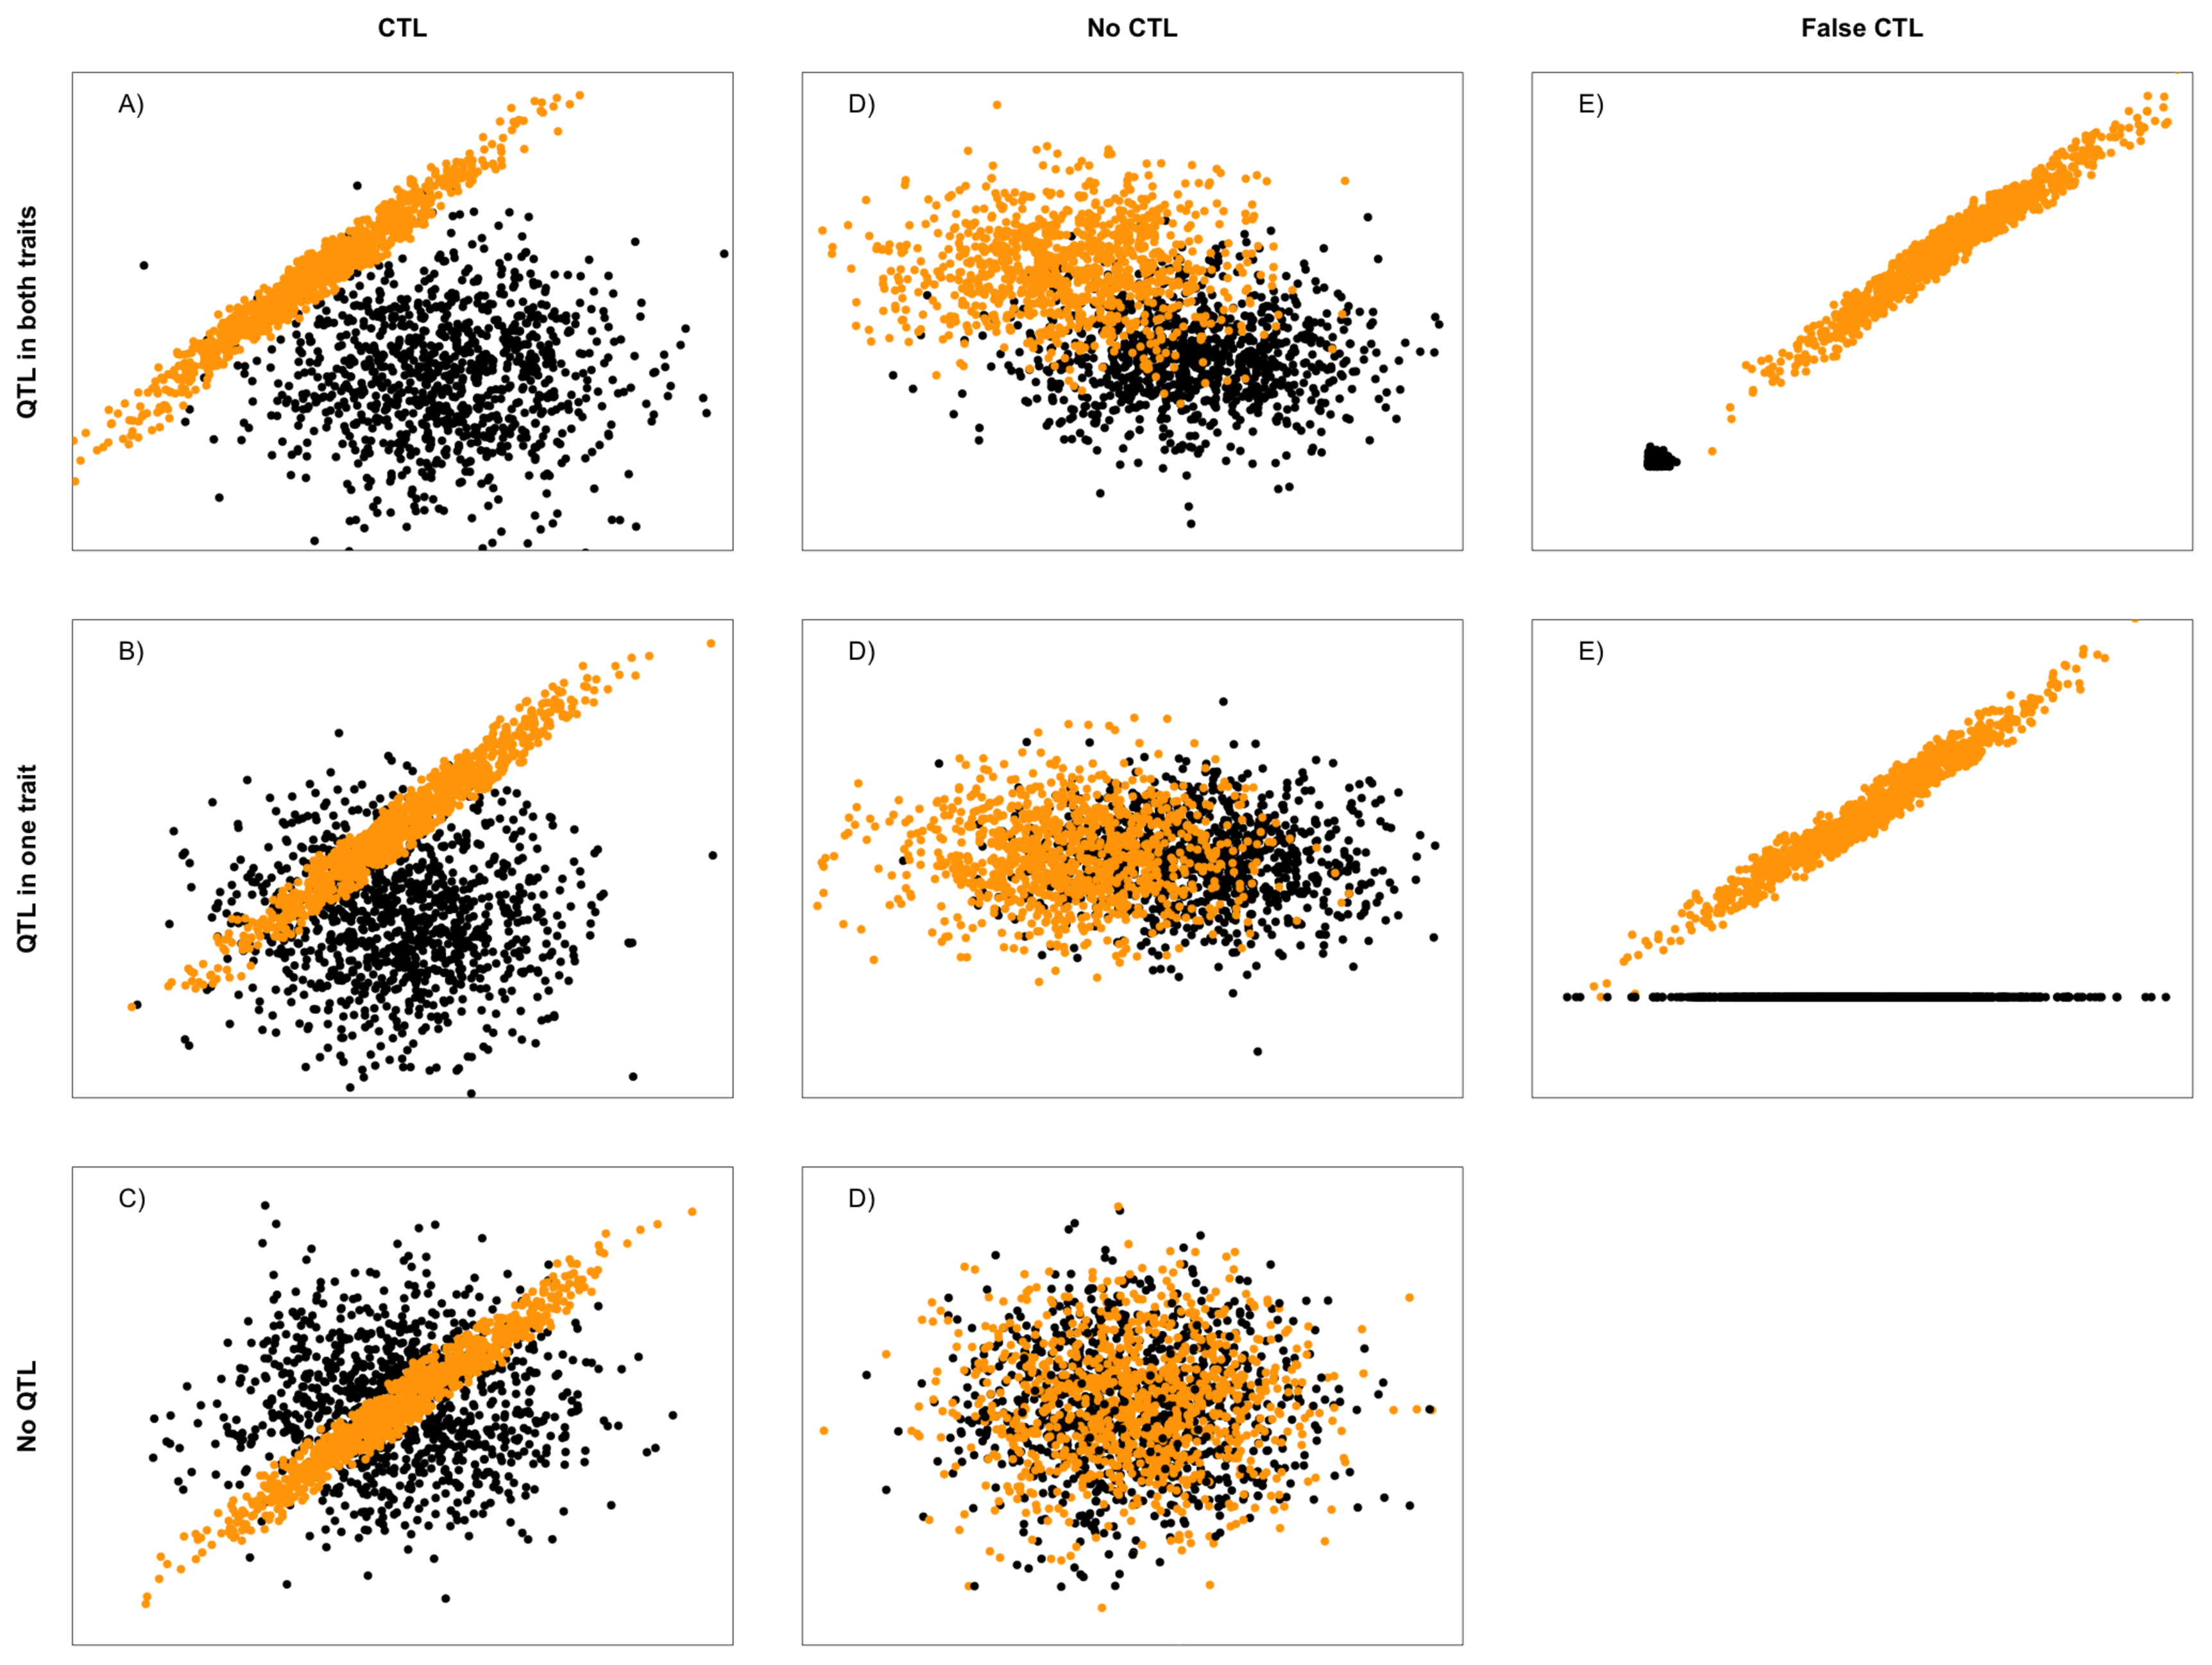
\includegraphics[width=0.9\textwidth]{eps/image_5_1.eps}
  \caption[MOLGENIS]
    {Many minor and major changes have to be written in software code before a 'standard' software infrastructure 
    accommodates a particular research. Using 'model-driven' development methods a bioinformatician only need to 
    model what is needed for his experiment using a therefore optimized domain specific language (DSL). Generators 
    quickly produce all the software logic to compose a full software infrastructure that accommodates these needs. 
    When experimental needs change, a bioinformatician can (re)run the same generator with an adapted model file 
    to quickly produce another variant of software infrastructure. This vastly reduces 'time-to-research' and 
    enables bioinformaticians to quickly develop a suite of software infrastructures, with each variant accommodating 
    a specific research task, while still on track to reuse, integrate and share the best standard features with 
    other labs and bioinformaticians.}
    \label{fig:modelDrivenDevelopment}
\end{figure}

The MOLGENIS toolkit is based on the method of model-driven development which emerged in the 1990s 
from the computer industry. Below we discuss the MOLGENIS' modeling language, the generators and 
reusable components. 

\subsubsection{Modeling language}
A custom MOLGENIS application can be defined in a single file. The file is written in MOLGENIS' 
modeling language. One can think of MOLGENIS' modeling language as a 'domain-specific language' 
\cite{Deursen:2002}, in this case to compose biosoftware infrastructures.

In most cases, knowledge of the DSL is all that is needed to produce a custom MOLGENIS application 
variant. The domain-specific language was implemented using XML so that model files can be edited 
using off-the-shelf XML editors. However, you may want to include hand-programmed components into 
a particular MOLGENIS instance. For example, for the eXtensible Genotype And Phenotype (XGAP) 
database application of MOLGENIS \cite{Swertz:2010a}, we developed a 'MatrixViewer' that builds on the generated 
components, which saved us the work of writing the plug-in from scratch. This requires a model 
sentence that points to the 'plug-in' (allowing it to be seamlessly integrated) as well as 
hand-programming of the plug-in itself.

\subsubsection{Reusable components}
Each MOLGENIS application follows the widely accepted three-layered architecture design of web 
applications. MOLGENIS' reusable components provide building blocks with a modular structure, which 
allows them to be assembled in diverse combinations, similar to prefabricated houses that are built 
from modular walls instead of bricks. Some building blocks are semi-finished and need to be 
'completed' before use (which is automated in MOLGENIS via the generators and inheritance). We based 
the design of MOLGENIS on industry-proven design patterns from the 'patterns for enterprise 
application architecture' (PEAA), a catalog of proven solutions for software design problems 
that we used as a guideline \cite{Fowler:2002}. The logic of the reusable components is implemented using 
Java (\url{http://java.sun.com/}); the HTML layout for the user interface is encoded in Freemarker 
templates (\url{http://freemarker.sourceforge.net/}); and the database back-end using MySQL, PostgreSQL 
or HSQLDB.

\begin{figure}[h!]
  \centering
  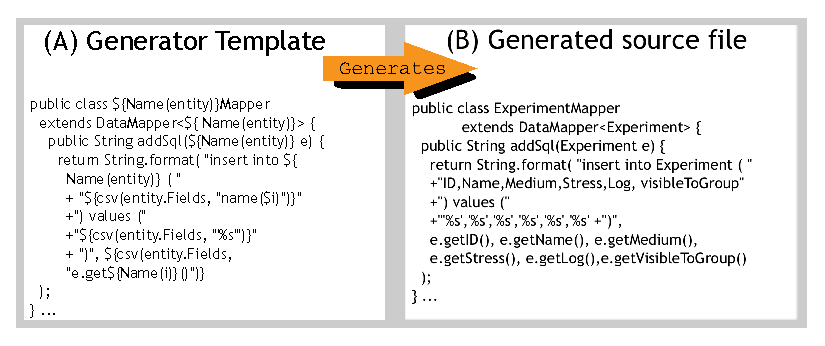
\includegraphics[width=1.0\textwidth]{eps/image_5_2.eps}
  \caption[Templates]
    {MOLGENIS generators are implemented as templates. This example shows the generator for a database component 
    (A). This template is applied to each <entity> in the model to generate many complete DataMappers that would 
    otherwise need to be written by hand. (B) shows an example of the generated source files, in this case for 
    <entity name="Experiment"> as described in Figure 1. The command \$Name(entity) translates to the name of the 
    entity ("Experiment") and command \${csv(\$entity.Fields, x)} means that command 'x' is applied to each field 
    of the entity and returned as a comma separated string (csv).}
	\label{fig:Generators}
\end{figure}

\subsubsection{Generators}
The generators are compact specifications of how each database feature should be implemented. 
The MOLGENIS toolkit now has over 20 generators, but normal users will never need to take a look 
inside. However, for readers wanting to create their own generators, figure \ref{fig:Generators} provides an example 
of the simple, text-based, generators we use. Each generator consists of two files: a Freemarker 
template that describes the code to be generated (similar to that shown in figure \ref{fig:Generators}a) and a Java 
'Generator' class that controls the generating process. A new generator can be developed as 
follows: First write some examples of the desired programs by hand, where possible using similar 
patterns and mark which parts are variable between them. Then copy one of these examples into 
a generator template (text file) and replace all variable parts with 'holes' that 
are to be filled by the code generator based on parameters from DSL. At each generation, the 
template is then automatically copied and the 'holes' filled, based on parameters described in 
the domain-specific language, saving much laborious manual work. 

\subsubsection{Results}
To start generating your own MOLGENIS application, you can download a ready-to-use 'workspace' 
from \url{http://www.molgenis.org/}, which can be edited using the commonly used Eclipse integrated 
development environment (IDE) tool (\url{http://www.eclipse.org/}). Extensive manuals are available to 
help install the Java, MySQL, Tomcat and Eclipse software needed and to learn how to walk through 
the Eclipse workspace to edit models and generate and run MOLGENIS instances; most new users can 
complete this part in about three hours. Below we summarize the output you can expect as well 
as recent experiences from using this toolbox. Detailed examples on how these features can be 
used to support actual microarray or genetical genomics experiments can be found in \cite{Swertz:2010a, Li:2009, Smedley:2008}.

After completing a MOLGENIS model and running the generator as described above, you have a 
ready-to-use software application. The features you get when running the generated result as 
a web application: a fully functional system where researchers can upload, manage, browse 
and query their biological data that conform to the model, optionally enhanced with analysis 
tools to explore and annotate (depending on the plug-ins).

\subsubsection{Applications of MOLGENIS}
Since the earliest MOLGENIS application \cite{Swertz:2004}, we have successfully evaluated use of 
the MOLGENIS toolkit to build a wide range of biomedical applications \cite{Swertz:2010a, Fredman:2002, 
Leu:2010, Li:2009, Smedley:2008}, ranging from sequencing to proteomics.A full list MOLGENIS applications 
can be found at \url{http://www.molgenis.org/}. Each of these MOLGENIS projects reported major benefits 
from the short cycle from model to running system to enable quick evaluation (500 lines of model XML 
replaces 15,000 lines of programming code) and use of the batch loading of data to evaluate how the newly 
built system works with real data. More often than not, MOLGENIS helped in finding inconsistencies in 
existing data that would otherwise have gone unnoticed, leading to experimental errors. In our experience, 
a typical MOLGENIS generator run gives you about 90\% of the application that is desired 'for free', with the 
remaining 10\% typically filled in using plug-ins that are written by hand. The MOLGENIS toolkit has also 
been used to extend or replace existing software applications: the ExtractModel tool allows you to generate 
a MOLGENIS application from an existing database, which can then be run side-by-side with code developed 
previously, providing the best of both generated and hand-written worlds.

\subsection{Storing extensible data (XGAP)}
We present an extensible software model for the genotype and phenotype community, XGAP. Readers 
can download XGAP (\url{http://www.xgap.org/}) or auto-generate a custom version using 
MOLGENIS with programming interfaces to R-software and web-services or user interfaces for 
biologists. XGAP has simple load formats for any type of genotype, epigenotype, transcript, 
protein, metabolite or other phenotype data. Current functionality includes tools ranging 
from eQTL analysis in mouse to genome-wide association studies in humans.

\subsubsection{XGAP - A minimal and extensible object model}
We developed the XGAP objectmodel to uniformly capture the wide variety of (future) genotype 
and phenotype data, building on generic standard model FuGE (Functional Genomics Experiment) 
\cite{Jones:2007} for describing the experimental 'metadata' on samples, protocols and experimental variables 
of functional genomics experiments, the OBO model (of the Open Biological and Biomedical 
Ontologies foundry for use of standard and controlled vocabularies and ontologies that ease 
integration \cite{Smith:2007}, and lessons learned from previous, profiling 
technology-specific modeling efforts \cite{Brazma:2006}.

Figure \ref{fig:XGAP}b shows the core components of a genotype-to-phenotype investigation: the biological 
subjects studied (for example, human individuals, mouse strains, plant tissue samples), the 
bio molecular protocols used (for example, Affymetrix, Illumina, Qiagen, liquid 
chromatography/mass spectrometry (LC/MS), Orbitrap, NMR), the trait data generated (usually 
data matrices with, for example, phenotype or transcript abundance data), the additional 
information on these traits (for example, genome location of a transcript, masses of LC/MS peaks), 
the wet-lab or computational protocols used (for example, MetaNetwork \cite{Fu:2007} in the case of QTL and
network analysis) and the derived data (for example, QTL likelihood curves).

\begin{figure}[ht!]
  \centering
  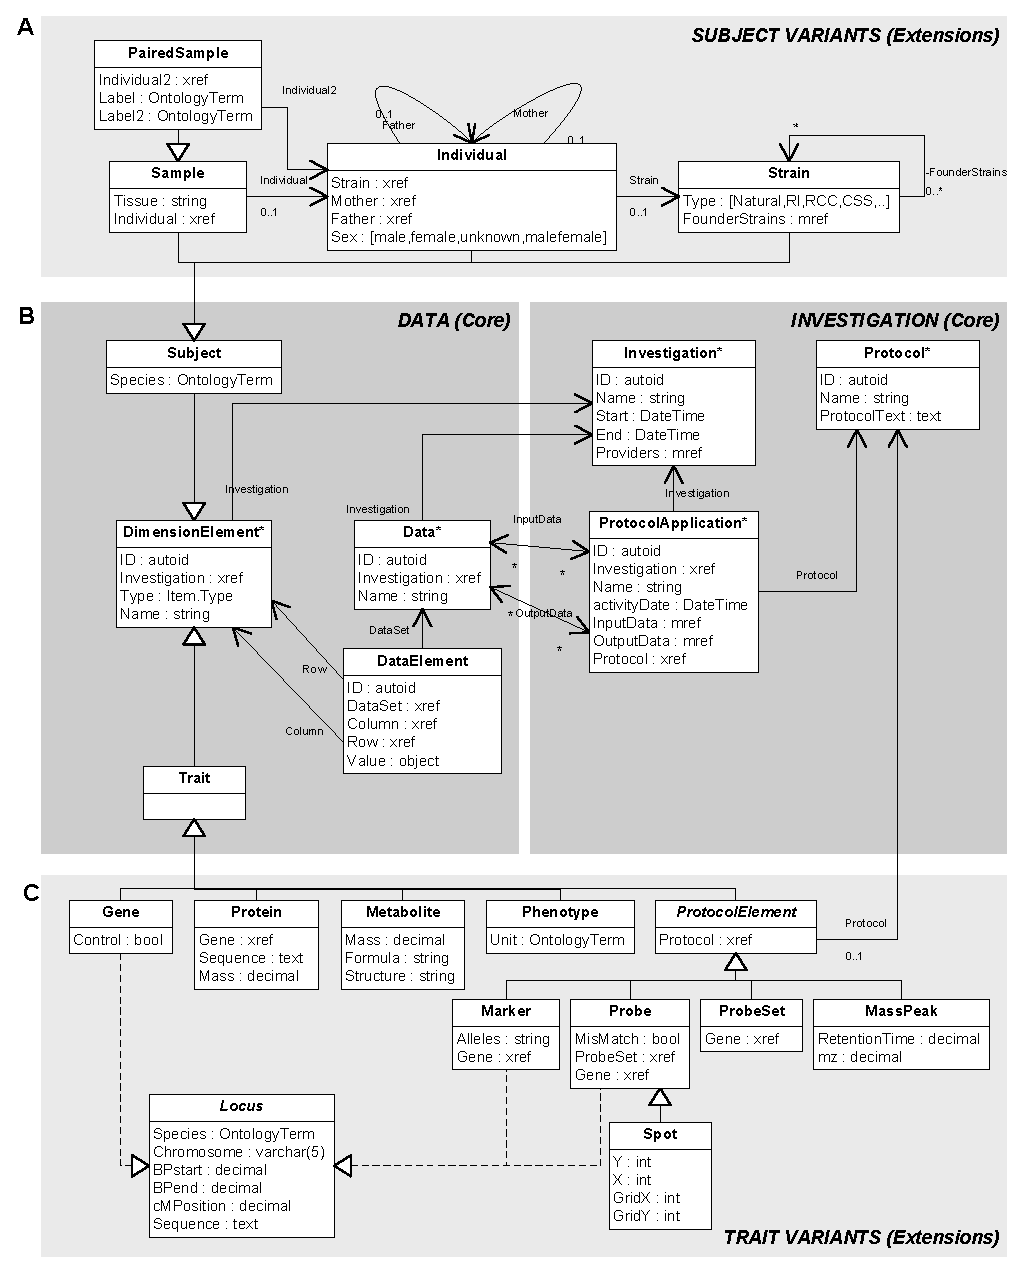
\includegraphics[width=0.75\textwidth]{eps/image_5_3.eps}
  \caption[XGAP.]
    {Experimental genotype and (molecular) phenotype data can be described using Subject, Trait, Data and DataElement; 
    the experimental procedures used can be described using Investigation, Protocol and ProtocolApplication (B). Specific 
    attributes and relationships can be added by extending core data types, e.g. Sample and Gene (A,C). The model is 
    described in UML: Arrows denote relationships (Data has a field Investigation that refers to Investigation ID); 
    Triangled lines denote inheritance (Metabolite inherits all properties ID, Name, Type from Trait, next to mass, 
    formula and structure); Triangled dotted lines denote use of interface (Spot 'implements' properties of Locus); 
    relationships are shown both as arrows and as properties ('xref' for one-to-many , 'mref' for many-to-many 
    relationships). Asterisk* marks FuGE derived types.}
    \label{fig:XGAP}
\end{figure}

We describe these biological components using FuGE data types and XGAP extensions thereof. 
Investigation binds all details of an investigation. Each investigation may apply a series 
of bio molecular \cite{Brown:2005} and computational \cite{Carey:2007,Alberts:2008,Fu:2007,Bhave:2007} 
Protocols. The applications of such Protocols are termed ProtocolApplications, which in the case 
of computational Protocols may require 
input Data and will deliver output Data.These data have the form of matrices, the DataElements 
of which have a row and a column index. Each row and column refers to a DimensionElement, 
being a particular Subject or a particular Trait, Table 2 illustrates the usage of these core 
data types. Figure \ref{fig:XGAP}a and \ref{fig:XGAP}c shows how the XGAP model can be extended to accommodate details on 
particular types of subjects and traits in a uniform way. A Trait can be a classical phenotype 
(for example, flowering - the flowering time is stored in the DataElement) or a bio molecular 
phenotype (for example, Gene X it's transcript abundance is stored in the DataElement). A 
Trait can also be a genotype (for example, Marker Y is a genomic feature observation that is 
stored in the DataElement). Genomic traits such as Gene, Marker and Probe all need additional 
information about their genome Locus to be provided. Similarly, a Subject can be a single 
Sample (for example, a labeled biomaterial as put on a microarray) and such a sample may 
originate from one particular Individual. It may also be a PairedSample when biomaterials come 
from two individuals - for example, if biomaterial has been pooled as in two-color microarrays. 
An individual belongs to a particular Strain. When new experiments are added new variants of 
Trait and Subject can be added in a similar way. Table 3 illustrates the generic usage of 
these extended data types.

Several standard data types were also inherited from FuGE to enable researchers to provide 
'Minimum Information' for QTLs and Association Studies such as defined in the MIQAS checklist 
 - a member of the Minimum Information for Biological and Biomedical Investigations (MIBBI) 
guideline effort \cite{Taylor:2008}

To support the increased demand for computational resources for included mapping routines we added 
high-level cluster and cloud management functions for computation. The scalable QTL mapping routines of 
\xqtlwb are written in R and C. The choice of R ties in with the general practice of using R for QTL 
mapping. The user interface includes direct access to the R interpreter. XGAP, \xqtlwb and MOLGENIS are 
open source software, and source code is transparentlystored and tracked in online source control 
repositories.

\subsubsection{XGAP - Conclusions and Discussion}
We present a minimal and extensible data infrastructure for the management and 
exchange of genotype-to-phenotype experiments, including an object model for genotype and 
phenotype data (XGAP-OM), a simple file format to exchange data using this model (XGAP-TAB) 
and easy-to-customize database software (XGAP-DB) that will help groups to directly use and 
adapt XGAP as a platform for their particular experimental data and analysis protocols. We 
successfully evaluated the XGAP model and software in a broad range of experiments: array 
data (gene expression, including tiling arrays for detection of alternative splicing, 
ChIP-on-chip for methylation, and genotyping arrays for SNP detection); proteomics and 
metabolomics data (liquid chromatography time of flight mass spectrometry (LC-QTOF MS), NMR); 
classical phenotype assays \cite{Heap:2009, Bystrykh:2005, Li:2006, Keurentjes:2006, Stranger:2007, Bailey:2008, Beamer:1999}; 
other assays for detection of genetic markers; and annotation information for panel, gene, 
sample and clone. 

Based on these experiences, we expect use of XGAP to help the community of genome-to-phenome 
researchers to share data and tools, notwithstanding large variations in their research aims. 
The XGAP data format can be used to represent and exchange all raw, intermediate and result 
data associated with an investigation, and an XGAP database, for instance, can be used as a 
platform to share both data and computational protocols (for example, written in the R 
statistical language) associated with a research publication in an open format. We envision 
a directory service to which XGAP users can publish metadata on their investigations either 
manually or automatically by configuring this option in the XGAP administration user interface. 
This directory service can then be used as an entry point for federated querying between the 
community of XGAPs to share data and tools. Groups that already have an infrastructure can 
assimilate XGAP to ease evolution of their existing software.

Next to their existing user tools, they can 'rewire' algorithms and visual tools to also use 
the MOLGENIS APIs as data backend. Thus, researchers still have the same features as before, 
plus the features provided by the generated infrastructure (for example, data management GUIs, 
R/API) and connected tools (for example, R packages developed elsewhere). Moreover, much 
less software code needs to be maintained by hand when replacing hand-written parts by 
MOLGENIS-generated parts,  allowing software engineers to add new features for researchers 
much more rapidly. We invite the broader community to join our efforts at the public XGAP.org 
wiki, mailing list and source code versioning system to evolve and share the best XGAP 
customizations and GUI/API 'plug-in' enhancements, to support the growing range of profiling 
technologies, create data pipelines between repositories, and to push developments in the 
directions that will most benefit research

\subsubsection{xQTL - Conclusions and Discussion}
\xqtlwb provides a total-solution for web-based analysis: Major QTL mapping routines are integrated 
for use by experienced and inexperienced users.  Tools such as a two-way communication with R/QTL 
\cite{Broman:2003, Arends:2010} enabling QTL mapping on XGAP formatted genotypes and phenotypes with 
QTL results stored back into \xqtlwb. Researchers can upload raw data, run analyses, explore 
mapped QTL and underlying information, and link-out to important databases. New algorithms can be 
flexibly added, immediately available to all users. Large analyses can be easily executed on a cluster, 
or in the Cloud. Future work include visualizations and search options to explore the results. We also 
had an EU-SYSGENET workshop that envisioned further integration of xQTL with analysis tools like HAPPY, 
databases like GeneNetwork, and the workflow manager TIQS \cite{Durrant:2012}.

\section{A worm database (WormQTL)}
WormQTL is one of the application developed using the xQTL workbench system. It is a public web portal 
for the management of all these new data and integrated development of suitable analysis tools. The 
web server provides a rich set of analysis tools available to use directly, based on R/qtl 
\cite{Broman:2003, Arends:2010}. Users can upload and share new R scripts as 'plugin' for colleagues 
in the community to use directly. New data can be uploaded and downloaded using XGAP-extensible 
text format for genotype and phenotypes\cite{Swertz:2010a}. All data and tools can be accessed 
via web user interfaces and programming interfaces to R, REST, and SOAP web services. Large 
consortia as well as individual researchers, can have a private area that is under embargo for 
publication. All software is free for download as MOLGENIS 'app' \cite{Swertz:2010b}. WormQTL is 
freely accessible without registration and is hosted on a large computational cluster enabling 
high throughput analyses to all at:\\
\url{http://www.wormqtl.org/}.

\subsection{Background}

Over the past 30 years, the metazoan \emph{Caenorhabditis elegans} has become a premier animal model for 
determining the genetic basis of quantitative traits \cite{Gaertner:2010, Kammenga:2008}. The 
extensive knowledge of molecular, cellular and neural bases of complex phenotypes makes 
\emph{C. elegans} an ideal system for the next endeavor: determining the role of natural genetic 
variation on system variation. These efforts have resulted in an accumulation of a valuable amount 
of phenotypic, high-throughput molecular and genotypic data across different developmental worm 
stages and environments in hundreds of strains \cite{Palopoli:2008, Kammenga:2007, Rockman:2010, 
McGrath:2009, Reddy:2009, Doroszuk:2009, Li:2010, Gutteling:2007, Vinuela:2010}. In addition, a similar wealth has been 
produced on hundreds of different \emph{C. elegans} wild isolates and other species \cite{Andersen:2012}. 
For example, \emph{C. briggsae} is an emerging model organism that allows evolutionary comparisons 
with \emph{C. elegans} and quantitative genetic exploration of its own unique biological 
attributes \cite{Ross:2011}.

This rapid increase in valuable data calls for an easily accessible database allowing for 
comparative analysis and meta-analysis within and across Caenorhabditis species \cite{Swertz:2007}. To 
facilitate this, we designed a public database repository for the worm community, WormQTL 
(\url{http://www.wormqtl.org/}). Driven by the PANACEA project of the systems biology program of 
the EU, its design was tuned to the needs of \emph{C. elegans} researchers via an intensive 
series of interactive design and user evaluation sessions on a mission to integrate all 
available data within the project.

As a result, data that were scattered across different platforms and databases can now be 
stored, downloaded, analysed and visualized in an easily and comprehensive way in WormQTL. 
On top, the database provides a set of user interfaced analysis tools to search the database 
and explore genotype-phenotype mapping based on R/qtl \cite{Broman:2003, Arends:2010}. New 
data can be uploaded and downloaded using the extensible plain text format for genotype and 
phenotypes, XGAP \cite{Swertz:2010a}. There is no limit to the type of data (from gene 
expression to protein, metabolite or cellular data) that can be accommodated because of its 
extensible design. All data and tools can be accessed via a public web user interface and 
programming interfaces to R and REST web services, which were built using the MOLGENIS 
biosoftware toolkit \cite{Swertz:2010b}. Moreover, users can upload and share more R 
scripts as 'plugin' for the colleagues in the community to use directly and run those on a 
computer cluster using software modules from xQTL workbench \cite{Arends:2012, Snoek:2012}; this requires 
login to prevent abuse. All software can be downloaded for free to be used, for example as 
local mirror of the database, and/or to host new studies.

All the software was built as open source, reusing and building on existing open source components 
as much as possible. WormQTL is freely accessible without registration and is hosted on a large 
computational cluster enabling high-throughput analyses. Below we detail the results and future plans.

\subsection{Results}
WormQTL is an online database platform for expression quantitative trait loci (eQTL) exploration 
to service the worm community and already provides many publicly available data sets \cite{Rockman:2010, 
Doroszuk:2009, Li:2006, Li:2010, Gutteling:2007, Vinuela:2010, Elvin:2011, Vinuela:2012}. New data 
sets can be uploaded using the XGAP plain file data format. Suitable help pages are provided. 
Currently, 38 public data sets have been loaded, of which the bulk is xQTL data on 500 strains 
(introgression lines, recombinant inbred lines (RILs), recombinant inbred advanced intercross lines 
and natural isolates), 55,000 transcripts, 1594 samples and 1579 markers (Table 1). With this 
combination of classical phenotypes, molecular profiles and genetics data sets, WormQTL contains 
all the 'genetical genomics' experiments published to our current knowledge (except for some tiling 
data). Using WormQTL, researchers can explore many xQTLs across the various studies in different 
conditions and ages and compare classical QTLs with xQTLs. The main interfaces are 'Find QTLs', 
'Genome browser' and 'Browse data'.

\begin{enumerate}\itemsep1pt
\item \emph{Find QTLs} - QTL is genomic regions associated with phenotypic variation and can be 
used to study the genetic architecture of traits and to detect potential phenotypic regulators. 
Recently, the number of QTLs and especially eQTL studies in \emph{C. elegans} has increased greatly. 
These eQTL studies consist of large data sets that, before WormQTL, were very difficult to access 
and perform a combined meta-analysis. Therefore, we provide easy access to most of the eQTL studies 
published, by search, browse and plot functions (Figure \ref{fig:xQTLworkbench}). We support relatively simple questions like 
'does my gene have an xQTL?' to more advanced ones like 'how do these genes fit into an xQTL network?'. 
All the matching genes, markers and traits found in the data sets are returned including links to 
WormBase and literature. Furthermore, WormQTL is the first portal for any species that allows comparison 
of eQTLs over multiple experiments and environments, giving insight in the plastic nature of genetic 
regulation.
\item \emph{Genome browser} - To find the genes that have a QTL on your favorite position, click 
'Genome browser'. Here, you can select from all the different releases of the University of California, 
Santa Cruz genome releases. You can add tracks from the designated experiments of interest. Then 
navigate to your favorite location (tip: use open in new window) and collect significant probe 
identifiers from that region.
\item \emph{Browse data} - Complete data sets and accompanying gene, sample and trait identifier 
lists can be browsed via the 'browse data' user interface. External identifiers anywhere in the 
data are automatically recognized and enhanced as linkouts to background information, such as links 
to Wormbase, NCBI, KEGG or Ensembl. All the annotation lists and data matrices can be browsed and 
searched in a tabular form and can be downloaded as plain text or Excel files. Readers can also 
download data sets or submit new data sets using the XGAP data format following examples described 
in the WormQTL help section. Also all data can be accessed programmatically from with R (as whole 
matrix or per row) or using REST web services, including filtering of the annotations (genes, probes, 
markers and phenotypes) and services to 'slice' individual lines out of the complete data sets to 
speed up download and (parallel) analyses. Alternatively, readers can request a login to upload 
data and new analysis scripts directly.
\end{enumerate}

\subsection{Conclusions and Discussion}
\subsubsection{Implementation}
All the software was implemented using the open source Molecular Genetics Information Systems 
MOLGENIS toolkit \cite{Swertz:2010a}, and in particular one previously existing MOLGENIS application, the 
extensible xQTL workbench \cite{Arends:2012} and the R/qtl QTL mapping and visualization package for the R 
language \cite{Broman:2003, Arends:2010}. The MOLGENIS toolkit is a Java-based software to generate tailored research 
infrastructure on demand \cite{Swertz:2007}. From a single 'blueprint' describing all biological data 
structures and user interfaces of the whole system, MOLGENIS auto generates a full application 
including user interface, database infrastructure and application programming interfaces 
(APIs) in R, REST and SOAP.

At the push of a button, MOLGENIS 'generators' automatically translates these models into a 
database, standard user interfaces for data queries and updates, upload/download tools for 
tab-delimited data and scriptable interfaces for programmers to users from within R and via 
web services. This greatly speeded up the initial software development and also enables rapid 
extension when, for example, new data types arrive. On top of this foundation, we build the 
WormQTL specific user interactions such as the 'Find QTLs' and the 'Genome browser' using 
MOLGENIS 'plug-in' mechanism and the visualizations and plots using the R interface. xQTL 
workbench is a scalable web platform for the mapping of QTLs at multiple levels: for example, 
gene expression (xQTL), protein abundance (pQTL), metabolite abundance (mQTL) and phenotype 
(phQTL) data. The xQTL workbench provided a set of previously developed user interfaces to 
run R/qtl mapping methods directly from within the WormQTL user interface, the ability to 
add new analysis procedures in R, data management and data format conversions, all greatly 
speeding up the generation of new xQTL profiles.

All the data sets were downloaded from their original sources and then formatted using the 
XGAP data format. XGAP is a simple text file format that uses a directory of tab-delimited 
files or one Excel file with multiple sheets to load lists of annotations and data matrices. 
The annotations list all the background information needed to run and interpret the analysis 
including, for example, genome position information, such as markers, genes, probes and 
strains. The data matrices describe all the raw, intermediate and result data, such as gene 
expression, genotypes and QTL P-values, with the row names and column names cross linking to 
the annotations. For example, gene expression is a matrix of 'gene' X 'sample'. Subsequently 
these data sets were loaded using the MOLGENIS/xQTL data import wizards, which check the 
files for correctness and give informative feedback if the data are not yet in a format that 
WormQTL can understand \cite{Swertz:2010a}. All the annotations are stored in tables in the database; the 
large data matrices are stored in a optimized binary format to speed up analyses and queries. 
This format is documented in the WormQTL manual to ease the submission of new data sets from 
the community. Finally, all the QTL profiles were recalculated according to the specification 
of the original, or slightly modified when needed, such as to include a previously missing 
wrongly labelled sample correction. In this process, we greatly benefitted from the integration 
with xQTL workbench, which enabled us to re-run all these analyses on the computer cluster 
and add new R analysis procedures when needed, simply from the user interface.

All software is available as open source on \url{http://github.com/molgenis/} for others to reuse 
locally, and related technical documentation is available from:\\ \url{http://www.xqtl.org/}, 
\url{http://www.rqtl.org/} and \url{http://www.molgenis.org/}.

\subsubsection{Future plans}
The current version of WormQTL (June 2012) is a comprehensive, versatile and flexible package. 
Follow-up plans of more extended versions with new tools and data depend on the demand by the 
users of WormQTL. We envisage that in the future, three types of new tools will be developed: 
(i) visualization tools, (ii) QTL mapping tools and (iii) candidate gene selection tools. Improved 
visualization tools might include plotting a phenotype against the marker at a certain position; 
so the two groups become visible at a QTL position. Also plots can be made showing transgression 
and heritability per microarray probe or gene or histograms of the phenotypic values (and include 
the parental values if available). Advanced QTL mapping tools might include multi-environment
/age mapping or genotype-by-environment analyses, developed in collaboration with the R/qtl team 
to enable automatic links to this software. The candidate gene selection tools would benefit from 
the most recent stable release of Wormbase \cite{Yook:2012}, the most widely used platform for worm biology. 
But also other sources of information like MODENCODE \cite{Gerstein:2010} or Wormnet 
\cite{Lee:2008} are likely to be connected with WormQTL. A candidate gene selection tool might be 
implemented in a next version 
of WormQTL as it is less easy to implement and often needs information beyond WormQTL. One can 
think of (i) which SNPs/genes/polymorphic genes/transcription factor binding sites and so forth 
are underlying a eQTL; (ii) which gene, underlying my xQTL, is linked to most of the genes 
having an xQTL; (iii) which genes are polymorphic and (iv) which other genotypes show a difference 
in expression and do they share polymorphisms with the parental strains of the RIL population 
that the xQTL was mapped in. Moreover, WormQTL can be easily expanded to other Caenorhabditis 
species \cite{Ross:2011}.

We believe that WormQTL, which will be continuously curated by the members of this international 
consortium, is a very attractive database for the growing community of quantitative genetics in 
worms researchers. We are committed to maintain data and software for the years to come and invite 
the community to add and share new data and ideas.

\subsection{Januari 2014: Update to wormQTL-HD}
Interactions between proteins are highly conserved across species. As a result, the molecular basis 
of multiple diseases affecting humans can be studied in model organisms that offer many alternative 
experimental opportunities. One such organism - \emph{Caenorhabditis elegans} - has been used to produce much 
molecular quantitative genetics and systems biology data over the past decade. We present WormQTLHD 
(Human Disease), a database that quantitatively and systematically links expression Quantitative 
Trait Loci (eQTL) findings in \emph{C. elegans} to gene-disease associations in man. WormQTLHD, available 
online at \url{http://www.wormqtl-hd.org/}, is a user-friendly set of tools to reveal functionally coherent
, evolutionary conserved gene networks. These can be used to predict novel gene-to-gene associations 
and the functions of genes underlying the disease of interest. We created a new database that links 
\emph{C. elegans} eQTL data sets to human diseases (34.337 gene-disease associations from OMIM, DGA, GWAS 
Central and NHGRI GWAS Catalogue) based on overlapping sets of orthologous genes associated to 
phenotypes in these two species. We utilized QTL results, high-throughput molecular phenotypes, 
classical phenotypes and genotype data covering different developmental stages and environments from 
WormQTL database. All software is available as open source, built on MOLGENIS and xQTL workbench. 




\chapter{Conclusion, Discussion and Future perspectives}
\thispagestyle{empty}
\emph{The last chapter we summarize the main themes of this thesis and look forward to the future.}
\null
\vfill

\begin{myexampleblock}{Parts of this chapter are adapted from:}
  \authors{Caroline Durrant, Morris A. Swertz, Rudi Alberts, Danny Arends, ... , Ritsert C. Jansen, Klaus Schughart, et al}\\
  \emph{ Bioinformatics tools and database resources for systems genetics analysis in mice 
         - a short review and an evaluation of future needs}\\
  \bold{Briefings in Bioinformatics} (2011)\\\\
\end{myexampleblock}

\newpage

This chapter highlights the conclusions of this thesis and there is a short discussion in 
which we look forward to the future of high throughput computing in systems genetics. We 
highlight the tools created in this thesis such as Pheno2Geno in section \ref{sect:Pheno2Geno} and xQTL 
workbench (\ref{sect:xQTLworkbench}). One of our current projects a new version of R/qtl called qtlHD 
is being discussed in section \ref{sect:qtlHD}. We end this chaper by highlighting some future challenges 
and solutions to these upcoming challenges in section \ref{sect:Future}

\section{Pheno2Geno}
\label{sect:Pheno2Geno}
Generating biomarkers from micro arrays, tilling arrays and RNAseq data is possible using 
mixture models. Phenotypes showing a dichotome 0/1 distribution with approximate equal 
proportions in, say, a RIL population can be used as genetic markers: genotypes can be 
called by connecting the 0/1 to the parental strains A/B. Such markers can then be used 
for de-novo construction of the genetic map or for saturation of a known genetic map 
\cite{West:2006, Truco:2013}.

Pheno2Geno provided highly optimized routines for generating genetics maps de-novo or to 
saturate existsing genetic maps. Pheno2Geno has output structures compatible with R/qtl 
\cite{Broman:2003, Arends:2010}, which provides further facilities for QTL mapping in 
inbred populations.

With the upcoming new version of R/qtl also the Pheno2Geno package will need to be redesigned 
to accomodate new requirements. These include expected changes such as: a more standalone package, 
further optimization of parallelisation, but also support for more cross types such as 
diversity outbred and/or collaborative cross mice. 

Other more uncertain requirements which might or might not come up are: The main developer 
of Pheno2Geno is currently working on polyploid species. Due to this investment of the first 
author in polyploid crops such as potatoes and tomatos, basic support for this could be added 
in upcoming versions of Pheno2Geno. The authors are committed to maintaining the package, 
and sourcecode is available open source making it easier to support future new requirements.

\section{xQTL workbench}
\label{sect:xQTLworkbench}
While the xQTL workbench system described in this thesis have the ability to absorb new 
analysis methods, consideration should be given to allow high flexibility. It will be 
difficult to anticipate new demands, requirements or new developments which could provide 
a better alternative than databases for data and R for analysis \cite{Arends:2012}.

The need for reliable but flexible infrastructure in systems genetics lead to the development of 
xQTL workbench. It combines, the flexibility of the MOLGENIS generator suite \cite{Swertz:2010b} 
with the most used computational and analytical tools for systems genetics (Such as: R/qtl 
\cite{Broman:2003, Arends:2010}, Plink \cite{Purcell:2007} and many other tools). Using R as 
esparanto between the different languages, this creates a system which systems geneticists can 
use to keep track of data generation and track their analysis. Aditionally using R as computational 
backend allows researchers to contribute their methods and algorithms back to the scientific 
community by uploading them into xQTL workbench.

\subsection{wormQTL and wormQTL - Human Disease}
The current version of WormQTLHD (August 2013) is a comprehensive and compendious database that 
enables molecular model organism data to be studied in the context of human diseases. Just as with 
WormQTL \cite{Snoek:2012}, we believe that WormQTLHD will be continuously curated by the members of 
the \emph{C. elegans} community. The results of the 'broad-sweep' disease-enrichment test in 
combination with the web tool will be of special interest to researchers in the human or worm 
domain. We believe these results could also be applied to prioritize the pathogenic variants 
increasingly being produced by next-generation sequencing in diagnostic labs. Genetic variants 
affecting human genes of unknown function may have worm orthologues that are part of human-worm 
phenologs and these may reveal or imply a role in a human disease \cite{Ostlund:2014}. Thus, 
through functionally conserved networks, missing information can be inferred and candidate genes 
can be selected via model organisms \cite{vanDerVelde:2014}.

The approach of WormQTLHD is conceptually similar to that described by Smedley et al. 
\cite{Smedley:2013}. They created an automated method called PhenoDigm to provide evidence about 
gene-disease associations by analysing phenotypic information. In their case, phenotypes consist of 
a collection of ontology terms, which are aligned and scored to derive an overall phenotype-similarity score. Using this 
method, known gene-phenotype associations in model organisms (mouse, zebrafish) can be transferred 
to other organisms such as man, and help us to understand the genetic cause of disease. This method 
works best when the model organism is physiologically close to man and has comparable classical 
phenotypes. It would therefore be less useful for \emph{C. elegans}. However, combining the molecular 
(WormQTLHD) and phenotypical (PhenoDigm) approaches results in a very powerful tool to discover 
novel gene-disease associations in man, especially when using physiologically close model organisms \cite{vanDerVelde:2014}.

We plan to further develop the WormQTLHD data and toolset. There might be more ways in which 
researchers would like to search through the large amounts of data, for example, based on custom 
lists of gene identifiers, or by combining tools such as finding QTLs within specific regions. 
The QTL plots could be improved or replaced with interactive graphs that are more informative and 
would allow the users to continue 'drilling down' in the data instead of returning to the home page 
for a new analysis with a different tool. Furthermore, we envisage close integration with other data 
sources and tools such as WormNet, R/qtl and GO Enrichment to provide even more biological context 
and analytical tools for the user.

Our new database makes this data attractive and easy-to-use for an even wider community of 
quantitative geneticists working on worms and man. We are committed to maintaining the data and 
software in the future and invite the community to add and share their new data and ideas. 

\section{R/qtlHD}
\label{sect:qtlHD}
Association and / or linkage analysis will continue to be the bread-and-butter analysis 
tool-set for systems geneticists of the future. However complex systems geneticists have 
to cope with the aquisition of data from diverse experimental designs and the analysis of 
these diverse data types. Requiring complex pipelines to analyse new complexity of the 
incoming data \cite{Trelles:2011}.

Environment x Genotype interaction analysis is also a future feature of R/qtl-HD. We looked at 
different experimental designs in in chapter \ref{sect:Metabolites} comparing three different 
designs: full block design, random design and generalized genetical genomics (GGG) design design 
\cite{Joosen:2013, Li:2009}. Besides showing that using a GGG experimental design for experiments 
gives higher statistical power to detect interactions between environmental and genetic variation 
compared to a random \cite{Joosen:2013}. We concluded that interaction models are a very powerful 
tool in understanding the complex interplay between genetics and (cellular) environments 
\cite{Joosen:2013} an should thus be considered as an important feature for a new version of the 
R/qtl software package.

Association analysis can be performed using different methods, e.g. single marker association 
mapping in outbred populations, interval mapping in inbred populations, or multiple QTL mapping. 
In this thesis we used multiple QTL mapping to find QTLs for classical traits related to 
germination of seeds in \emph{A. thaliana}. We have shown an increase in QTL detection power 
of MQM versus standard single marker QTL mapping \cite{Jansen:1994a, Joosen:2011}. This shows 
that more genetic loci are involved in germination of seeds then previously known. Additionally 
Multiple QTL mapping should be implemented into R/qtl-HD besides standard single marker mapping 
to allow more powerful detection of QTL.

Increase in data size disqualifies R as main analysis platform. R is  not be the most suitable 
platform for the analysis of next generation high throughput data. While the R environment is 
well suited to scientific computing and performing statistical analysis, when big data is involved 
it is not the fastest or most optimized language available. When dealing with high throughput 
data obtained from RNA-seq, exome sequencing or Bi-sulfite sequencing datasize quickly become 
the limiting factor for software written in R. Because R/qtl-HD is aimed at QTL analysis of 
high-density, high-throughput data, R is not a suitable language for the computation parts of 
the algorithm.

R/qtlHD is written in the high performance D programming language. D is chosen as primairy 
language because it is created to perform safe and high throughput numerical analyses. D uses 
a C like syntax \cite{Alexandrescu:2011} providing a familiar syntax for the R/qtl developers, 
most of which come from a C/C++ background making D the language of choice for R/qtl-HD. 
Additional features of D include:
\begin{enumerate}\itemsep1pt
\item \emph{Improved code quality} - This makes the code more maintainability and more readable code is 
easier to reason about and optimize code, leading to improved performance of algorithms.
\item \emph{D allows to call C} - D allows to call C (and a limited subset of C++) functions directly. This 
allows to re-use previously written R/qtl code (written in R and C) \cite{RQTLGuide:2009}.
\item \emph{Build in unit testing} - Unit testing is build into the D programming language, allowing 
programmers to use the power of unit- and regression testing to build a test suite without the need 
for external tools or frameworks.
\item \emph{Concurrency and Actors} - The D language provides high level patterns such as Actors and 
Message Passing to deal with parrallelization of code. Unlike other languages, this is a build in 
feature of the language, this allows the standard D library to use safe lock free concurreny mechanisms \cite{Alexandrescu:2011}.
\item \emph{Static typing} - D requires types (e.g. Integer, Float, Double) to be declared and known 
at compile time, this improves readability of code and reduces the risk for run-time type errors of the system.
\item \emph{Compile Time Function Execution} - Compile time function execution (CTFE) is a feature 
that allows to build look up tables at compile time. This greatly reduces the runtime of algorithms, 
by pre-calculating common cases \cite{ArendsBlog:2012}.
\end{enumerate}
These are the main reasons for the R/qtl development team to favor D over R.

The current version of R/qtl provides many tools for genetic map construction, but also several historical 
methods for QTL mapping. R/qtl-HD will not provide a multitude of methods but focus more on the high speed 
analysis of data using stable and proven methods such as Haley-Knott regression \cite{Haley:1992} and analysis of variance.
Additional features such as genetic map construction and validation are not high priority when converting 
the R/qtl software into a more optimized language. R/qtl-HD is designed for mapping huge volumes of phenotypes 
onto medium to large genetic maps \cite{Trelles:2011}.

Furthermore multiple QTL mapping (MQM) from R/qtl will also be converted into the D programming language.
The MQM routine has proven to be a useful addition to the R/qtl toolkit and with the new implementation 
of R/qtl as R/qtlHD, we aim to improve the usefulness even more. The major limitation in MQM is the 
additional computational load when compared to single marker QTL mapping \cite{Arends:2010}. The R/qtl 
development team is committed to 1) add the MQM routine to the R/qtlHD package and 2) provide further 
optimization to MQM to allow it to handle even large volumes of phenotype and genetic data. 

An overview of the features planned for the R/qtl-HD package:
\begin{enumerate}\itemsep1pt
\item \emph{Universal input format} - Based on our experiences with XGAP \cite{Swertz:2010a} and xQTL workbench 
\cite{Arends:2012}, QTAB was developed as input format for Rqtl-HD. A testing version of QTAB was implemented in 
R/qtl-HD by Pjotr Prins. The QTAB format aims to provide a universal solution to the storage of genotype and genetic 
maps in inbred populations.
\item \emph{Single marker QTL mapping} - R/qtl HD aims to provide the most common single marker mapping methods. 
These methods will be optimized to work with huge amounts of phenotype data, created by new technologies such as: 
Tilling arrays, RNA-seq and/or exome sequencing.
\item \emph{Multiple QTL mapping} - We aim to implement multiple QTL mapping and as such benefit from the added 
advantages of the D language such as: Reduced memory usage during runtime and less run time due to the fact that 
it is easier to use parrallel computation in D.
\item \emph{Gene x Environment} - We aim to implement a generic approach for Gene x Environment analysis, we believe 
this type of analysis to become more and more important in the future to untangle te relationship between genome and 
phenome.
\item \emph{R interface} - Current R/qtl users should be able to switch to R/qtl-HD, while keeping their familiar 
R interface. in an ideal world current users should automatically switch to R/qtl-HD without them noticing.
\item \emph{BioRuby} - Bio-packages are being created for many languages (Python, Perl, etc), Ruby is a new and 
upcoming language in the scientific field. R/qtl HD aims to provide bindings to the BioRuby project \cite{Goto:2010} 
as as proof of concept, other BioPackages could model their own bindings on these Ruby bindings.
\item \emph{Compatibility} - R/qtl-HD aims to be compatible with the following operating systems: Mac OS X, 
Microsoft Windows and Debian Linux.
\end{enumerate}

R/qtlHD is developed as open source community software, currently a very limited version 
is available as preview for download. A development version is available from: 
\url{http://github.com/qtlHD/}

Further adaptations of the system currently not being considered, but which might be interesting opportunities for 
future work include: Integration of mapping analysis tools with genomic annotation and sequence data, generalization 
of analysis frameworks to accommodate not only mouse and human data but also data from other model organisms with 
different (non inbred) genetic pedigree structures, such as pets (e.g. cats, fish, dogs), farm animals (e.g. horses, 
cattle, pigs) and plants (e.g. arabidopsis, brassica, maize). Additional tools for genetic map construction might 
also be considered for inclusion, but currently are not a priority, since the current R package provides tools for 
this.

\section{Future perspectives}
\label{sect:Future}
With increasing scale of experimental data being produced in the lab, it will not be 
sufficient to have analysis software as simple downloads, because the researcher will 
also need sizable compute and storage power \cite{Schadt:2010}. Thus, researchers will 
need easy access to 'software as a service' such as cloud computing. Additionally storage 
of raw and pre-processed data is starting to become increasingly more expensive with 
increasing data sizes involved, this will be discussed in sections \ref{subsect:ClusterComputing} 
and \ref{sect:CloudComputing}. Additionally reproducability of analysis methodologies which 
involves a large code base is proving to be increasingly more difficult, when version of 
software and dependancies change. A small discussion which highlights current solutions 
to this problem of reproducability is found in section \ref{sect:CodeSharing} about sharing 
code and collaborating on large code bases.

How this increasing demand for storage and computational power can be satisfied in the future remains 
an unanswered question. Although federate computing providers (such as Target or EU-grid) can help 
researcher in their need for big computing solutions in the near future. This is also not a 
universal solution, while the speed of data production is currently higher then the speed of 
CPU improvement \cite{Moore:1998, Editorial:2009, Shah:2013}. Two solutions which are 
currently already available are highlighted here: Cluster and cloud computing might be able to 
solve the Big Data questions researchers currently face.

\subsection{Cluster computing}
\label{subsect:ClusterComputing}
A cluster is a collection of computers dedicated to solving a computational task by divide 
and conquer \cite{Silva:1999, Qiu:2010}. It basically means to having a basic relatively 
homogeneous software available on demand, on suitable compute and storage hardware. Hardware 
resources are divided by an internal scheduling system amongst different tasks form different 
users. However, users in general have little control over the computational environment, 
because administration of the cluster and the scheduling system put constraints on the usage 
of cluster. Computing clusters can be fashioned from different types of hardware, such as:
\begin{itemize}
  \item Ad-hoc networks composed of many heterogeneous relatively cheap systems such as: FPGA, and/or CPU, ARM core
  \item Dedicated computer clusters, such as TARGET or national GRIDs, where usually a homogenous system of linux machines is used for computational tasks.
  \item Video card cluster for linear algebra, utilizing the power of many simple GPU cores for dedicated tasks.
\end{itemize}
Compute clusters do not have to be homogeneous in nature. Though in many cases there will 
homogeneity to provide users with a stable computational environment to perform their tasks. 
Additionally the use of hardware can limit the usage of a cluster to a certain range of 
computational tasks such as GPUs or dedicated ARM cores.

\subsection{Cloud computing}
\label{sect:CloudComputing}
The term cloud is used in many different ways, and there is little consensus on what a cloud 
exactly is \cite{Foster:2008}. It essence it means to have software available 
on demand, on suitable compute and storage hardware, with the user being charged for the time 
that it is being used. Following the concept of the leading cloud provider Amazon, it refers 
in practice to use of a virtual Linux machine, i.e. a virtual compute server with Linux 
preinitialized, hosted within some large compute infrastructure, with complete freedom to be 
customized by the user although not for free \cite{Trelles:2011}.

Many commercial, national and local compute centers are also increasingly providing computer
server capacity in a cloud fashion. This makes these virtual machines an easy method to distribute 
software and computation without the need for all participating computational nodes to install 
software. Thus, the infrastructure is specified jointly \cite{Foster:2008} but for the actual computation every 
partner can be private with their data. This approach grants enormous computational power to 
everyone with minimal preparation - once that a shared image is finalized \cite{Krampis:2012}.

The setup of such a compute cloud is not trivial but several initiatives are underway to ease 
this process. At the workshop, the bioinformatics work-group tested the packaging system provided by 
the Debian Med initiative as a method to create a cloud and could be consider this as a seed 
for an image to then be publicly shared. Instructions to create such images were prepared for 
the workshop and made available at:\\
\url{http://wiki.debian.org/DebianMed/LiveCD/}
 
Using this method the cloud infrastructure can be transferred to local computer clusters 
if desired. Every participant has access to the server and can grant access to collaborators 
without having to pay the hosting fees. When complete, this server image can be ported to 
cloud providers such as: Amazon, Rackspace to be reused by other researchers.

\subsection{Code sharing and versioning}
\label{sect:CodeSharing}
Access and sharing of software code of all aforementioned tools is essential to avoid 
duplication of efforts, promote interoperability and to really collaborate within the mouse 
genetics bioinformatics community. Only then does it really become clear what is available 
and how there can be data and software flow between projects.

An example tool to facilitate such sharing and collaboration on code level is Git: Git 
allows users to follow updates (versions) of software packages and easily provide feedback \cite{Git:2007}. 
The most recent stable R version of R/qtl and qtlHD can be found as a Git repository, Git 
helps to control versions for the authors and facilitate compatibility with other packages 
such as QTL-bim and Pheno2Geno. Although most users will generally find the last stable version 
(Git master branch) the most useful and user-friendly, it is possible to download a 
development branch to get familiar with the new features being prepared for the next version.

An alternative to Git is Subversion (SVN) \cite{SVN:2002}. GeneNetwork code was developed 
using Subversion with Python as its primary language. GeneNetwork code and a shell (partial) 
database are available on Source Forge \cite{GeneNetwork:1994, GeneNetwork:2004}:\\
\url{http://sourceforge.org/projects/genenetwork/}

The mapping and permutation code used by GeneNetwork for real time analysis is based on fast 
Haley-Knott approximations \cite{Haley:1992} and is available on Source Forge:\\
\url{http://qtlreaper.sourceforge.net}

xQTL and XGAP code were also developed in Subversion \cite{SVN:2002} using Java as its primary language and 
R for its analysis interfaces. XGAP code and binaries are all available as open source at
\url{http://www.xgap.org/} and \url{http://www.molgenis.org/}. From a developer's perspective both Git and
SVN are equally well-suited for publishing code and may be used in parallel. However recently 
in 2012 also the entire MOLGENIS software suite (MOLGENIS, XGAP, xQTL workbench) was transfered 
to Git and moved to \url{http://www.github.com/} to get more online exposure, and remove the need 
to host an internal SVN server.

Additionally, all software developed described in this thesis is also written and developed 
using Git for source code control, and is available from Github at:\\
\url{http://github.com/DannyArends/}


\chapter{Additional for Dissertation}
\thispagestyle{empty}
\emph{The last chapter containing some additional things needed for a complete 
dissertation document required for a promotion at the University of Groningen.}
\null
\vfill
\newpage

\section{Dutch Summary / Nederlandse Samenvatting}
Systeem genetica is een inter disciplinair veld wat zch bezig houdt met de gevolgen van 
genetische variatie op alle biomoleculaire niveaus een biologisch systeem. Het effect van 
deze genetische variantie leidt tot verschillen in phenotypes, zoals opbrengt en resistentie. 
Het doel van systeem genetica is het indelen van de oorzaken van deze geobserveerde 
phenotypische variatie in drie categorieen: Genetische effecten, omgevings effecten en 
(random) residuele error variantie. Door netwerken te bouwen van interacties tussen 
alle biomoleculaire niveaus probeert systeem genetics complexe phenotypes te verklaren uit 
het samenspel tussen deze niveaus.

Biologie gebruikt natuurlijke variatie en genetische pertubatie om de componenten te ontrafelen
die phenotypische variatie veroorzaken, deze metingen gecombineert met pertubatie van verschillende 
omgevingsfactoren staat ons toe om de invloed van verschillende effecten zoals omgeving en 
omgeving x genotype te bepalen. Experimenteel ontwerp and statistiek kunnen gebruikt worden om 
de error variantie te minimaliseren.

Hoofdstuk \ref{chap:introduction} becat een korte historische introductie over systeem genetics, 
In de volgende hoofdstukken van deze thesis laten de bijdrages zien van deze thesis aan systeem genetics.

Hoofdstuk \ref{chap:pheno2geno} (Pheno2Geno) gaat over het construeren van genetische kaarten vanuit grootschalige 
omics datasets. De theory achter het maken van genetische kaarten is ongeveer 100 jaar oud. Maar 
software beschikbaar voor het maken van genetische kaarten in model organismes is nog 
vaak nog niet aangepast aan nieuwe ontwikkelingen zoals multicore computers en cluster computing. 
Pheno2Geno is software voor het maken can genetische kaarten uit Big Data verkregen door 
experimenten de gebruik maken van tilling arrays of RNA sequence experimenten.

Hoofdstuk \ref{chap:mqm} omschrijft de implementatie van het multiple QTL mapping algorithme ontwikkeld door 
R. C. Jansen in R/qtl. Hiermee voegen we een nieuw algorithme aan de R/qtl toolset toe, een 
toolset speciaal ontwikkeld voor het mappen van QTLs in ingeteelde (mouse) populations. R/qtl 
vormt de basis van meerdere tools die allemaal gebouwd zijn rond een gedeelde datastructuur. 
Deze structuur maakt het makkelijk om software aan te passen en nieuwe tools toe te voegen.
Door de vele tools, kunnen onderzoekers snel wisselen van methode wanneer dit vereist is of 
verschillende methodes vergelijken zonder een nieuw software pakket te hoeven leren.

Huidige werkzaamheden over het gebruik van \emph{verschillen in correlatie} om interactie 
netwerken te genereren en celtype specifieke QTL effecten op te sporen wordt beschreven in 
hoofdstuk \ref{chap:ctlmapping}. Correlated Traits Locus analyse (of CTL mapping) laat 
onderzoekers toe om genetische loci te vinden die geassocieerd zijn met correlatie verschillen 
tussen segregerende phenotypes. Een variant op deze methode is waardevol gebleken om cel 
type specifieke eQTL effecten te ontdekken. Deze effecten kunnen worden gebruikt om mengsels 
van cellen te ontwarren zo als in geheel bloed gen expressie data.

In hoofdstuk \ref{chap:xqtlwormbench} presenteren we onze idee\"en voor een generiek opslag en rekenplatform 
voor systeem genetica. Ons demo systeem xQTL workbench wordt momenteel gebruikt als een 
backend voor de WormQTL en WormQTL-HD databases. In xQTL workbench kunnen gebruikers hun 
gegevens op slaan en delen in een lokale of webomgeving, en lopen analyse over datasets met 
behulp van de kracht van gedistribueerde computing. Het wordt standaard geleverd met QTL 
mapping tools, zoals: R/QTL, Plink en qtlbim maar ook biedt het een web inferface, data 
importers, API's en visualisaties.

Ik vertrouw erop dat je geniet van het lezen van dit proefschrift, zoals ik heb genoten van het maken 
ervan.

\newpage
\section{Abbreviations and Acronyms}
{\footnotesize
\begin{tabular}{ l l }
API:         & Application Programming Interface\\
BC:          & Backcross \\
bp:          & Base pair(s) \\
cM:          & centi Morgan \\
CIM:         & Composite interval mapping \\
CPNN:        & Collaborative computing project for NMR\\
CSV:         & Comma separated values\\
CTL:         & Correlated traits locus \\
DesignGG:    & Experimental design of genetical genomics software\\
DRY:         & Principle of don't repeat yourself\\
DSL:         & Domain Specific Language\\
EBI:         & European Bioinformatics Institute\\
FINDIS:      & Finish disease database\\
GEMs:        & Gene expression based genetic marker\\
GEN2PHEN:    & EU project to unify human and model organism genetic variation databases\\
GMOD:        & Generic model organism database project\\
GUI:         & Graphical user interface\\
GWAS:        & Genome Wide Association Study\\
GWL:         & Genome Wide Linkage analysis\\
HGVBaseG2P:  & Human genome variation database of genotype-to-phenotype information\\
HTML:        & Hypertext markup language\\
IDE:         & Integrated Development Environment\\
JAR:         & Java Software Archive\\
LGPL:        & Lesser general public license\\
MAGE-TAB:    & Microarray gene expression tab delimited file format\\
Mbp:         & Mega base pairs = 1.000.000 bp \\
MOLGENIS:    & Molecular genetics information systems toolkit\\
NordicDB:    & Nordic Control Cohort Database\\
OBF:         & Open Bioinformatics Foundation\\
OntoCAT:     & Ontology common API toolkit\\
PEAA:        & Patterns for enterprise application architecture\\
QTL:         & Quantitative trait locus\\
RDF:         & Resource description format\\
REST:        & Representative state transfer web services\\
RIL:         & Recombinant inbred line \\
SNP:         & Single Nucleotide Polymorphism\\
SOAP:        & Simple Object Access Protocol\\
SQL:         & Structured Query Language\\
UML:         & Uniform data Modeling Language\\
WAR:         & Web Application aRchive file\\
XML:         & Extensible Markup Language\\
XGAP:        & Extensible genotype and phenotype software platform. 
\end{tabular}
}
\newpage

\section{Acknowledgements}
Knowledge is in the end based on acknowledgement\\
- Ludwig Wittgenstein (1889 - 1951)\\\\

There are many people who need to be thanked and acknowledged, 
here are the people who made the cut:

{\bf Ritsert C. Jansen} to whom I owe my life in science, thank you for giving me this chance 
to work in your group and develop my skills in research and education. {\bf Anna Mulder}, my 
girlfriend, for all the times I left you and {\bf Oscar} (our cat) for my science endavours. 
Thank you for your trust in me and giving me a home to come home to.
My family {\bf Bert}, {\bf Dinie}, {\bf Johan} and {\bf Jos\'{e}} for their support and understanding. 

{\bf Pjotr Prins} Always forgotten, Never Ignored. 

I would like to thank all the people past and present at the {\bf Groningen BioInformatics Centre} 
(GBIC) group for putting up with me. In particular, {\bf Yang Li} for your mentorship and all the 
vibrant discussions we had at GBIC and {\bf Joeri van der Velde} my friend and coworker for all 
the good times hacking on Java and R in Haren. 

{\bf Morris Swertz} my co-promotor, you were a great help when writing chapter \ref{chap:xqtlwormbench} 
and always made me feel at home at GCC. Also all the guys from the {\bf Genomics Coordination 
Centre} (GCC) department for all the 'end of sprints', presentations, discussions, coffee served by {\bf Roan Kanninga} and beers. 
{\bf Frank Johannes} my other co-promotor, for reading this thesis and proving me with usefull feedback, 
Additionally I would like to thank everyone from {\bf JohannesLab} for participating during Tuesday morning 
seminars and journal clubs. 

{\bf Lude Franke} and {\bf Harm-Jan Westra} for the very informative collaboration on the 
human GWA study (chapter \ref{sec:cellspecificeqtl}), I learned a LOT from you, and am 
extremely thankful for your help with the final chapters of this thesis. 

I have been very lucky to meet and work together with some of the cleverest minds in animal breeding 
and genetics. Being able to discuss my ideas with people such as {\bf Karl Broman}, {\bf Gary Churchill}, 
{\bf Allen Attie} and {\bf Brian Yandell} made me push myself to the limits and beyond. I would like 
to thank all of you for the nice times I had across the pacific ocean. 
Additionally I was lucky to have good collaboration with Wageningen University, especially {\bf Wilko 
Ligterink}, {\bf Henk Hilhort} and {\bf Ronny Joosen} for doing the \emph{Arabidopsis thaliana} 
experiments, and trusted me to analyze their data. I learned a lot especially about the more 'biological' 
parts of this thesis. 

Furthermore I have had the pleasure to work with many dedicated students along the way: 
My student {\bf Konrad Zych} for his dedication and help with Pheno2Geno and chapter \ref{chap:pheno2geno}. 
{\bf Mark de Haan} for his work on the xQTL workbench system and the review work on Pheno2Geno.
{\bf Yalan Bi} for working on the \emph{A. thaliana} gene expression data and alternative splicing 
work, which unfortunately was not finished in time for this thesis. And {\bf Adriaan van der Graaf} for 
showing me that even jocks can be turned into nerds. And naturally all the other students I have been 
privileged to work with during these last years.

I would like to thank the {\bf European Union} for setting up the {\bf SysGeNet} network, I've met 
many people and learned a lot about the mouse community in Europe. Especially I would like to thank 
{\bf Klaus Schughart} for starting and maintaining the network, and {\bf Leonard Schalkwyk} for 
inviting me to the UK for a lecture series at King's College.

{\bf Richard Stremme} and {\bf Evert van der Velde} for always being available after work for a beer and providing
entertainment and the needed distraction when being fed up with writing this thesis.
The {\bf University of Groningen} (RUG) for educating me and providing me with an place to do my research. And 
finally the {\bf University Medical Centre Groningen} (UMCG) for the pleasant working atmosphere and good lunches.

\newpage

\section{About the author}
\subsection{Curriculum Vitae}

\begin{wrapfigure}{r}{0.4\textwidth}
  \centering
  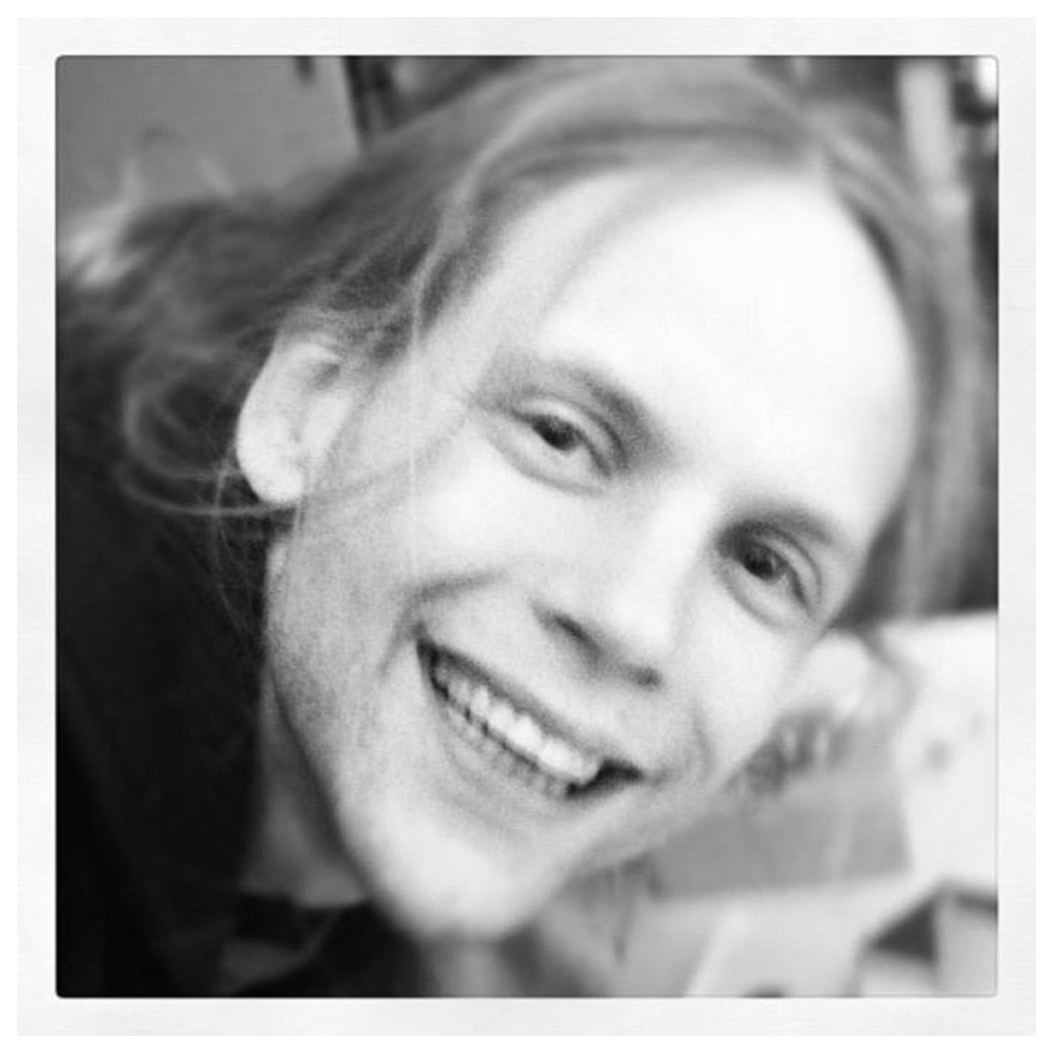
\includegraphics[width=0.3\textwidth]{eps/image_6_1.eps}
\end{wrapfigure}

Danny Arends was born on the 15th of Juli 1983 in the city of Zwolle located in the heart 
of the Netherlands. After moving twice, Danny went to an elementary school situated in 
Heiligerlee, a minuscule hamlet in the north of Holland in the province of Groningen. 

The small school was a perfect match for young Danny during his childhood. Here he quickly 
fell in love with mathematics, and the wondrous world of numbers and patterns. With the 
advent of computers at the elementary school, the love for computers and their inner 
workings also began to develop.

Heiligerlee is located next to a small forest called 'De Hoogte', this forest was used 
by Danny and friends on a daily basis to build tree huts and by using snow balls in winter 
wage war on kids from the other school in Heiligerlee. The forest combined with growing up 
amidst animals on a farm-like residence sparked young Danny his intrests in biology.

After elementary school Danny went to the Ubbo Emmius lyceum in Stadskanaal (Groningen). 
The large scale VWO was a big change compared to the small elementary school. Long hours at school 
together with a long bus ride to and from school, made for long days. Fortunately new 
friends were made in the class room and during the long bus rides. Danny finished high 
school after 6 years, taking mostly exact courses such as mathematics, physics and chemistry.

At 17, a university degree should be the next step in his career. Because of his interests 
in computers, Danny decided that computer science would be a good match. This turned out 
to be not so true. While deeply intrigued by the subject of computational machines, he 
was not satisfied by just studying the workings of a machine build by man.

After two years of Computer science at the University of Groningen, Danny decided it was time 
for a change. Computer science was replaced by Life Science \& Technologie, a bachelor which 
was recently formed as a collaboration between the Biology faculty and Medical Sciences.

He finished his bachelor in record tempo, partly due to the exemptions obtained from 
doing two years of computer science. A Master in molecular biology was quickly selected after
being introduced to bioinformatics at GBIC during a previous bachelor project. The molecular 
biology master allowed for customization of the courses followed, and bioinformatics became the main 
theme in all of the master theses produced. The first thesis: "Machine learning to predict 
transcriptional regulation in prokaryotes" was produced in the group of Oscar Kuipers. 
The second master thesis about 'R/QTL, MQM algorithm' was done in the lab of Ritsert C. Jansen 
under the supervision of Pjotr Prins.

Parts of this second master project are found in this thesis (chapter \ref{chap:mqm}).
After graduating his university master Cum Laude. Danny started a PHD project at Ritsert 
C. Jansen at the Groningen Bioinformatics Centre with a focus on the use of bioinformatic 
tools to handle current challenges in genetics and statistics. These four years of research 
at the GBIC have resulted in the thesis you are currently reading.\\\\

\newpage

\subsection{List of Publications}

\subsubsection*{Authored:}
   R/qtl: high throughput Multiple QTL mapping\\
  \authors{Danny Arends*, Pjotr Prins*, Ritsert C. Jansen and Karl W. Broman}\\
  \bold{Bioinformatics} (2010)\\\\
  Visualizing the genetic landscape of Arabidopsis seed performance\\
  \authors{Ronny V. L. Joosen*, Danny Arends*, Leo Willems, Wilco Ligterink, 
           Henk Hilhorst and Ritsert C. Jansen}\\
  \bold{Plant Physiology} (2011)\\\\
  Large scale NGS pipelines using the MOLGENIS platform: processing the Genome of the Netherlands\\
  \authors{Heorgy V. Byelas*, Danny Arends*, Freerk van Dijk, K. Joeri van der Velde, Laurent 
            Francioli, Martijn Dijkstra, Alexandros Kanterakis, Ishtiaq Ahmad, David van Enckvoort, 
            Leon Mei, Peter Horvatovich, other members of BBMRI-NL, NBIC and Target, Morris A. Swertz}\\
  \bold{Proceeding of: 12th Annual Bioinformatics Open Source Conference BOSC 2011} (2011)\\\\
  xQTL workbench: a scalable web environment for multi-level QTL analysis\\
  \authors{Danny Arends*, K. Joeri van der Velde*, Pjotr Prins, Karl W. Broman, 
           Steffen Moller, Ritsert C. Jansen and Morris A. Swertz}\\
  \bold{Bioinformatics} (2012)\\\\
  WormQTL: Public archive and analysis web portal for natural variation data in Caenorhabditis spp\\
  \authors{L. Basten Snoek*, K. Joeri Van der Velde*, Danny Arends*, Yang Li*, 
           Antje Beyer, Mark Elvin, Jasmin Fisher, Alex Hajnal, Michael O 
           Hengartner, Gino B. Poulin, Miriam Rodriguez, Tobias Schmid, 
           Sabine Schrimpf, Feng Xue, Ritsert C. Jansen, Jan E. Kammenga 
           and Morris A. Swertz}\\
  \bold{Nucleic Acids Research} (2012)\\\\
  Identifying genotype-by-environment interactions in the metabolism of germinating Arabidopsis seeds 
  using Generalized Genetical Genomics\\
  \authors{Ronny V. L. Joosen*, Danny Arends*, Yang Li*, Leo Willems, Joost J. B. Keurentjes, Wilco Ligterink, 
           Ritsert C. Jansen and Henk Hilhorst}\\
  \bold{Plant Physiology} (2013)\\\\
  Cell-type specific eQTL analysis without the need to sort cells\\
  \authors{Harm-Jan Westra*, Danny Arends*, ..., Ritsert C. Jansen and Lude Franke}\\
  \bold{Nature Methods} (2014)

\subsubsection*{Co-Authored:}
  The MOLGENIS toolkit: rapid prototyping of biosoftware at the push of a button\\
  \authors{Morris A Swertz, Martijn Dijkstra, Tomasz Adamusiak,  Joeri K van der Velde, 
           Alexandros Kanterakis, Erik T. Roos, Joris Lops, Gudmundur A. Thorisson, 
           Danny Arends, George Byelas, Juha Muilu, Anthony J. Brookes, Engbert O. de Brock, 
           Ritsert C Jansen and Helen Parkinson}\\
  \bold{BMC Bioinformatics} (2010)\\\\
  XGAP: a uniform and extensible data model and software platform for genotype and phenotype experiments\\
  \authors{Morris A Swertz, K. Joeri van der Velde, Bruno M Tesson, Richard A Scheltema, 
           Danny Arends, Gonzalo Vera, Rudi Alberts, Martijn Dijkstra, Paul Schofield, 
           Klaus Schughart, John M. Hancock, Damian Smedley, Katy Wolstencroft, Carole 
           Goble, Engbert O. de Brock, Andrew R Jones, Helen E Parkinson and Ritsert C Jansen}\\
  \bold{Genome Biology} (2010)\\\\
  SYSGENET: a meeting report from a new European network for systems genetics\\
  \authors{Klaus Schughart, Danny Arends, P. Andreux, R. Balling, Pjotr Prins, et al.}\\
  \bold{Mammalian Genome} (2010)\\\\
  Trans-eQTLs Reveal that Independent Genetic Variants Associated With a Complex Phenotype Converge on 
  Intermediate Genes, with a Major Role for the HLA\\
  \authors{Rudolf SN Fehrmann, Ritsert C. Jansen, Jan H. Veldink, Harm-Jan Westra, Danny Arends,
           Marc Jan Bonder, Jingyuan Fu, Patrick Deelen, Harry J. M. Groen, Asia Smolonska, 
           Rinse K. Weersma, Robert M. W. Hofstra, Wim A. Buurman, ... , Lude Franke}\\
  \bold{Plos Genetics} (2011)\\\\
  Bioinformatics tools and database resources for systems genetics analysis in mice - a short review 
  and an evaluation of future needs\\
  \authors{Caroline Durrant, Morris A. Swertz, Rudi Alberts, Danny Arends, Steffen Möller, 
           Richard Mott, Pjotr Prins, K. Joeri van der Velde, Ritsert C. Jansen and 
           Klaus Schughart}\\
  \bold{Briefings in Bioinformatics} (2011)\\\\
  WormQTLHD - a web database for linking human disease to natural variation data in C. elegans\\
  \authors{K. Joeri van der Velde*, Mark de Haan, Konrad Zych, Danny Arends, L. Basten Snoek, 
           Jan E. Kammenga, Ritsert C. Jansen, Morris A. Swertz and Yang Li}\\
  \bold{Nucleic Acids Research} (2014)

\subsubsection*{In Preparation/ Under Review / In Press:}
  Pheno2Geno - High throughput generation of genetic markers and maps from molecular phenotypes\\
  \authors{Konrad Zych, K. Joeri van der Velde, Ronny V. L. Joosen, Wilco Ligterink, Ritsert C Jansen 
           and Danny Arends}\\
  \bold{BMC Bioinformatics} (201X)\\\\
  Correlated Traits Locus mapping\\
  \authors{Danny Arends, Pjotr Prins, Harm-Jan Westra, Yang Li, Lude Franke and Ritsert C. Jansen}\\
  \bold{Unknown} (201X)\\\\
  TiQS: web environment for expression QTL analysis\\
  \authors{Steffen M\"oller, Ren\'e Sch\"onfelder, Hajo Krabbenh\"oft, Benedikt Bauer, Yask Gupta, 
           Pjotr Prins, Danny Arends, et al.}\\
  \bold{BMC Bioinformatics} (201X)\\\\
  Multiple QTL mapping of cardiac collagen deposition in an F2 population of Scn5a mutant mice reveals 
  interaction between Fgf1 and Pdlim3, Gpr158 \& Itga6\\
  \authors{Elisabeth M. Lodder, Brendon P. Scicluna, L. Beekman, Danny Arends, et al.}\\
  \bold{Genome Research} (201X)\\\\
  Regulatory Network of Secondary Metabolism in Brassica rapa: An Insight In The Glucosinolate Pathway
  \authors{Dunia Pino del Carpio, Ram Kumar Basnet, Danny Arends, Ke lin, Ric CH de Vos, Dorotha Muth, 
           Jan Kodde, Kim Boutilier, Johan Bucher, Xiaowu Wang, Ritsert Jansen, Guusje Bonnema}\\
  \bold{Plos One} (201X)

\subsection*{Acknowledged in:}
  Probability genotype imputation method and integrated weighted lasso for QTL identification\\
  \authors{Nino Demetrashvili, Edwin R van den Heuvel and Ernst C Wit}\\
  \bold{BMC Genetics}, 14:125 (2013)\\\\   
  DesignGG: an R-package and web tool for the optimal design of genetical genomics experiments\\
  \authors{Yang Li, Morris A Swertz, Gonzalo Vera, Jingyuan Fu, Rainer Breitling and Ritsert C Jansen}\\
  \bold{BMC Bioinformatics}, 10:188 (2009)\\\\
  Generalizing genetical genomics: getting added value from environmental perturbation\\
  \authors{Yang Li, Rainer Breitling and Ritsert C. Jansen}\\
  \bold{Trends in Genetics}, 24:518-524 (2008)

\subsection{List of Presentations}
R/xqtl: High throughput modeling, mapping and exploration of Big Data\\
SYSGENET meeting - Braunschweig, April 2010\\\\
Introduction into QTL analysis\\
Dynamic Presentation - University of Groningen, Aug 2010\\\\
MQM and HPC for R/qtl\\
CSBG meeting - Wageningen University, Sept 2010\\\\
Introduction into QTL mapping - Bioinformatics I\\
University of Groningen, June 2011\\\\
(Re)Construction of genetic maps from gene expression data\\
GBIC - University of Groningen, July 2011\\\\
R/qtl for Big Data\\
MIT Department of Biology, invited by Jeroen PJ Saeij\\
MIT, Boston (MA), May 2011\\\\
The Challenge of Big Data Genetical Genomics\\
NCSA, invited by Victor Jongeneel and Chris Fields\\
NCSA, Urbana (IL), May 2011\\\\
Introduction into QTL mapping - Learning From nature (LFN)\\
Wageningen University, Feb 2012\\\\
Computer practical / tutorial - Learning From nature (LFN)\\
Wageningen University, Feb 2012\\\\
Introduction into R and R/qtl\\
Summer Course - King's college, Sept 2013\\\\

\subsection{List of Posters}
User friendly cluster computing for QTL analysis\\
  \authors{Danny Arends, Joeri v/d velde}\\
  \bold{ISMB} July 2010 - Boston, USA\\\\
Multiple QTL mapping poster\\
  \authors{Danny Arends, Pjotr Prins,Karl W. Broman and Ritsert C. Jansen}\\
  \bold{GBIC day} September 2010 - Groningen, The Netherlands\\\\
Pheno2Geno poster\\
  \authors{Konrad Zych, Danny Arends, Ritsert C. Jansen}\\
  \bold{NBIC} April 2012 - Lunteren, The Netherlands\\\\
Pheno2Geno poster\\
  \authors{Konrad Zych, Danny Arends, Ritsert C. Jansen}\\
  \bold{ECCB / ESCS} Sept 2012 - Basel, Swiss\\\\
GWAS in potato\\
  \authors{Konrad Zych, Danny Arends, Ritsert C. Jansen}\\
  \bold{Kings College} Sept 2013 - London, UK

\subsection{Awards}
1st place Poster Award 'Pheno2Geno' at ESCS2012 Basel (Swiss) (2012)\\
Travel Grant by NBIC for ISMB in Boston (MA, USA) (2010)\\
2nd place Poster Award xQTL workbench NBIC Conference (Lunteren) (2010)\\
Travel Grant 'Short course on system genetics' in Bar Harbor (MA, USA) (2009) by JAX laboratory\\


\bibliographystyle{unsrt85}
\addcontentsline{toc}{chapter}{Bibliography}
{\footnotesize
\bibliography{Thesis}
}
\end{document}

